\chapter{Computing Disparity Confidence Intervals}\label{chap:epistemic_uncertainty}
The previous chapter detailed the propagation of uncertainty in a stereo matching problem, using the \acrshort{sad} function to compute the cost volume. However, real cases of stereo matching usually do not use such simple cost functions, but rather more complex ones. In particular, the CARS pipeline that will process the \acrshort{co3d} data will use the CENSUS and MC-CNN cost functions  \cite{zabih_non-parametric_1994,zbontar_stereo_2016} to compute the cost volume, followed by a \acrshort{sgm} regularization. Those methods produce far better results and are thus favored for stereo pipelines \cite{hirschmuller_evaluation_2009}. Unfortunately, propagating the uncertainty to those cost functions and their regularization as we did in the previous chapter would currently be too complex and computationally heavy for a practical use. The same observation can be made for any deep learning method \cite{laga_survey_2022} as the data is processed through many consecutive layers. Furthermore, the previous chapter was restricted to the propagation of the uncertainty from input images to the cost volume, but did not attempt to quantify the uncertainty of the stereo matching process itself, \ie the algorithm's ability to identify the correct disparity. A bad performing stereo matching algorithm can produce errors of great magnitude regardless of the uncertainty on input images, while a more advanced algorithm may perform well despite noisy input images. Using the semantics of this thesis, we will refer to the uncertainty of the stereo algorithm itself as its epistemic uncertainty. Indeed, it does not result from any aleatoric process, but rather a lack of knowledge on how to automatically identify the correct disparity.

This epistemic uncertainty in stereo matching has been the subject of many studies in the literature \cite{hu_quantitative_2012,  poggi_confidence_2021,wang_uncertainty_2022}, designed for so-called ``classical methods'' using cost volumes obtained from cost functions, or for learning-based methods. This uncertainty is quantified using ``confidence measures'', associating a value between $0$ and $1$ to each predicted disparity; $0$ meaning that the prediction should be questioned, and $1$ meaning that the prediction is most certainly correct. We refer to \Cref{sec:uncertainty_pandora} for more details on confidence measures in stereo matching pipelines. In this chapter, we will study how possibility distributions are able to model the epistemic uncertainty associated with a cost volume, and then deduce disparity confidence intervals from the possibility distribution. This approach is complementary to classical confidence estimations, as it is not meant to indicate whether we trust a prediction, but rather to provide information on \textit{where} the correct disparity is likely to be. We then propagate those disparity confidence intervals in the rest of the stereo pipeline to obtain elevation confidence intervals, and evaluate their performance. Following discussions with users and experts working at \acrshort{cnes}, \acrshort{ign} and more generally in the AI4GEO consortium (\url{https://www.ai4geo.eu/}), we decided to aim for an objective of $90\%$ of correct confidence intervals. This chapter takes up work and data published in \cite{malinowski_robust_2024-1}.

\section{Producing Confidence Intervals}
This section will detail the method developed to create disparity confidence intervals in the stereo matching step of the pipeline. We will use possibility distributions to model the uncertainty associated with the available information and deduce confidence intervals from it.

It is important to keep in mind that we want intervals as accurate as possible, while staying relatively small. Indeed, it would be easy to reach a $100\%$ accuracy by simply extending the intervals to the whole range of considered disparities. However, the intervals would not contain any relevant information. We therefore must maintain a trade-off between the accuracy of the intervals and their size. As stated previously, we fixed ourselves a $90\%$ accuracy objective. As for the criteria of maintaining small intervals, we will introduce in \Cref{sec:metrics_disparity} different metrics to quantify their size for further evaluation. Different parameters will be introduced in our method, and we chose their values accordingly with the accuracy/size trade-off mentioned above. We will also study different configurations of those parameters in the \hyperref[chap:annex]{Annex}.

\subsection{Possibility Distributions as Uncertain Models for Cost Curves}
In this section, we will detail how possibility distributions can be used to model the epistemic uncertainty associated with cost curves. We first present a quick reminder of concepts and notations regarding cost volumes presented in \Cref{sec:stereo_matching}, as we will base our model on them. Cost volume based approaches, considered here, compare every pixel from the left image $I_L$ to pixels from the same row in the right image $I_R$, in a given disparity range. The comparison is done using a cost function $f$, measuring the dissimilarity between two windows centered around pixels $p$ and $q$. All evaluations using this cost function are stored in a cost volume $C_V$:
\begin{align}
	C_V(\rowcol, ~d) = f(I_L(\rowcol), I_R(\rowcol+d))
\end{align}
where $d$ is the considered disparity. In this chapter, we consider that the cost volume undergoes a \acrshort{sgm} regularization step, which modifies its values to take into account more global information as presented in \Cref{sec:cost_volume_optimization}. Based on the observation that the disparity map is usually piece-wise regular in a scene, \acrshort{sgm} regularization has been designed to increase the cost of disparities for which no consensus exists among neighboring pixels. This way, only disparities that seem plausible and relatively regular compared to neighboring disparities are favored in the cost volume.

For every pixel $(\rowcol)$ from the left image, we refer to its cost curve as the cost volume at coordinates $(row,~col)$ for every considered disparity $d$, \ie the cost volume for which we fixed the first two variables. Cost curves are of great importance, as we estimate the disparity of a pixel solely based on its cost curve. Indeed, we define the predicted disparity $\tilde{d}$ of a pixel $(\rowcol)$ as:
\begin{align}
	\tilde{d} = \argmin_d C_V(\rowcol, ~d)
\end{align} 
In the next figures, we use the same configuration for computing the cost volume, \ie CENSUS cost function with \acrshort{sgm} regularization. \Cref{fig:tuto_dense_matching} presents a cost curve and its true disparity. We can see that the true disparity can be correctly estimated by looking at the minimum of the cost curve.
 
\begin{figure}
    \centering
    \begin{subfigure}[t]{0.073\linewidth}
        \centering
        
\includegraphics[width=\linewidth]{Images/Chap_5/tuto_left_patch.png}
        \caption{}
        \label{fig:tuto_a}
    \end{subfigure}
    \hfill\begin{subfigure}[t]{\linewidth}
        \flushright
        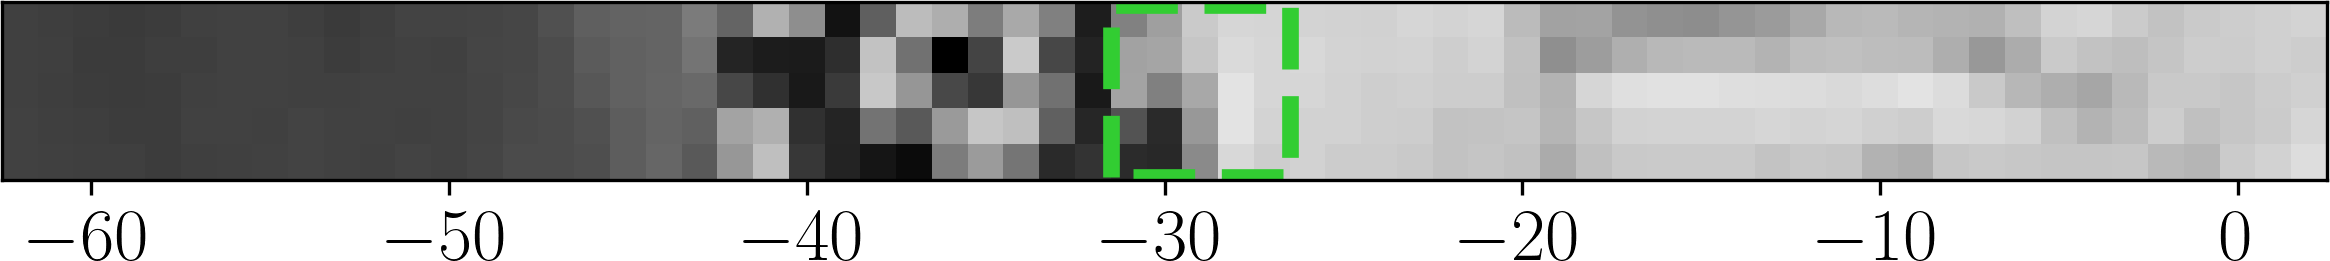
\includegraphics[width=0.927\linewidth]{Images/Chap_5/tuto_right_patch.png}
        \caption{}
        \label{fig:tuto_b}
    \end{subfigure}
    \begin{subfigure}[t]{\linewidth}
        \centering
        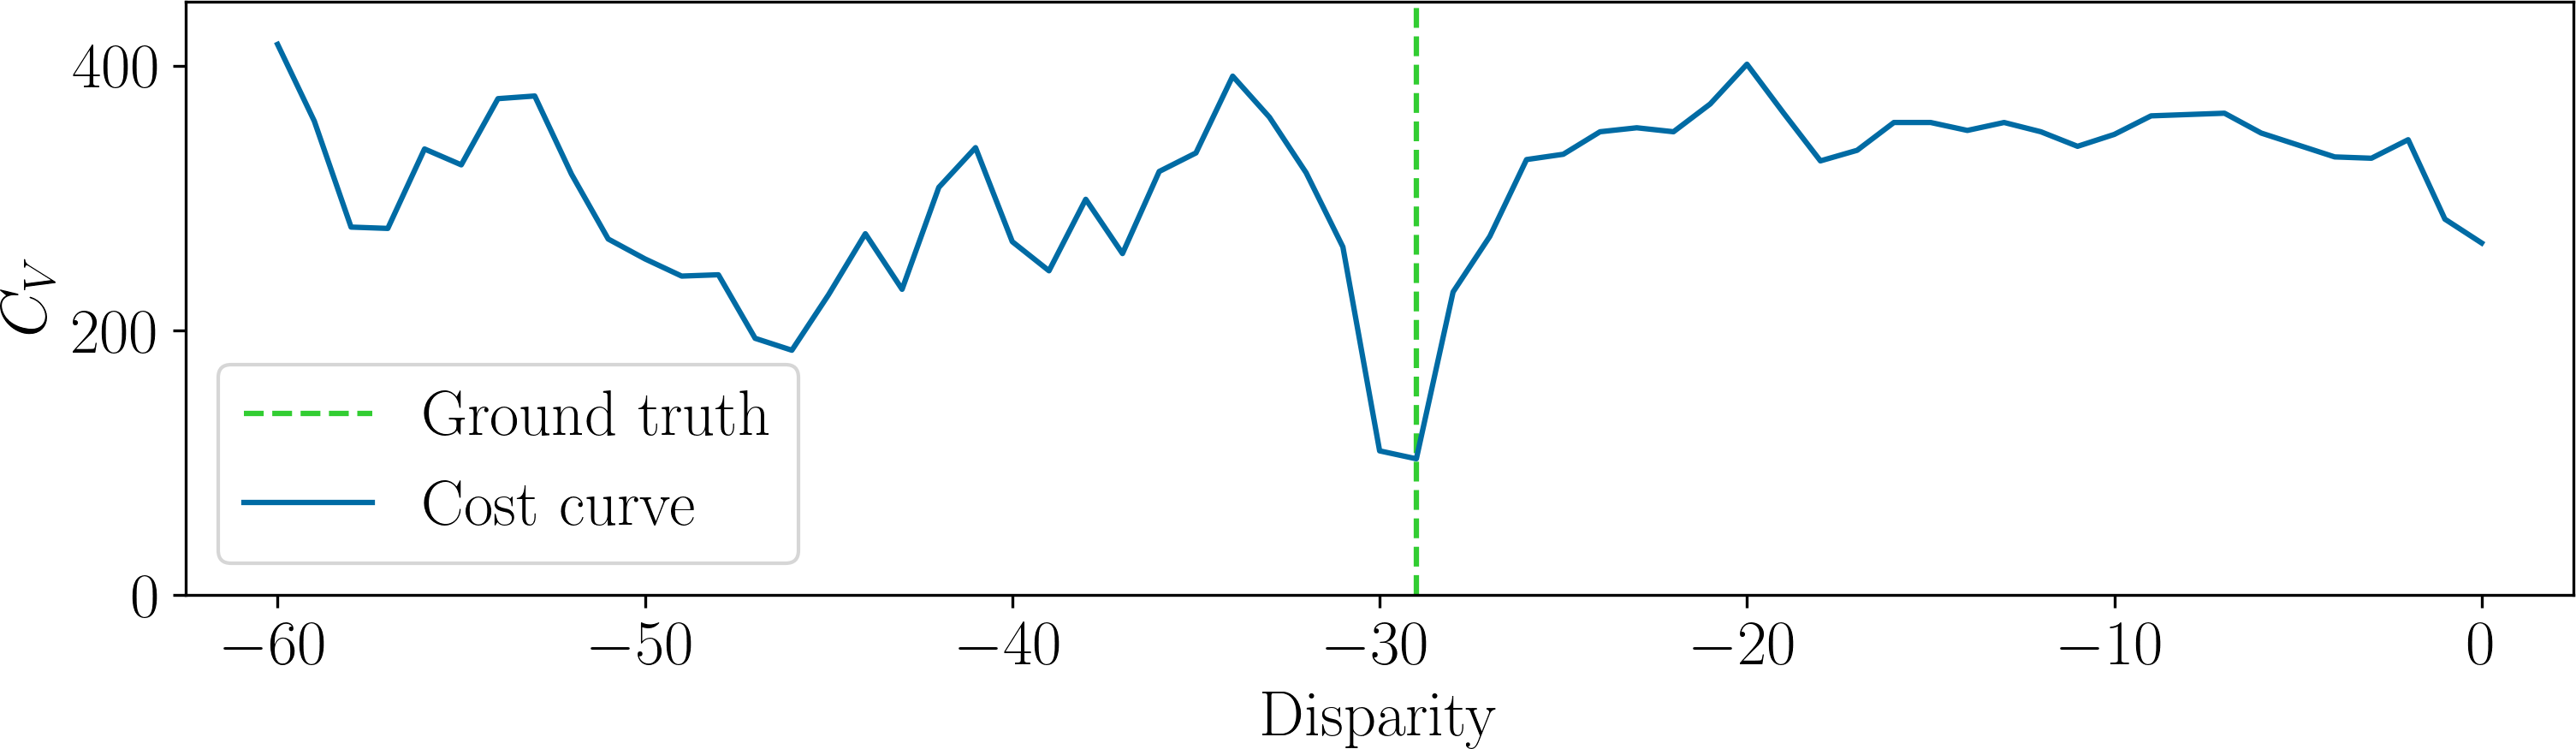
\includegraphics[width=\linewidth]{Images/Chap_5/tuto_cost_curve.png}
        \caption{Cost curve}
        \label{fig:tuto_c}
    \end{subfigure}
    \caption{\subref{fig:tuto_c}: cost curve obtained from comparing a patch of the left image from \subref{fig:tuto_a} to patches of the right image from \subref{fig:tuto_b}. The matching patch and its corresponding true disparity are indicated using dashed green lines.}
    \label{fig:tuto_dense_matching}
\end{figure}

In the following, we propose to consider possibility distributions to model the uncertainty associated with the choice of the predicted disparity from a cost curve. The values taken by possibility distributions will be based on the available information, \ie the values of the cost volume. Before getting into details, let us justify this model. Possibility distributions are relatively simple models to use in comparison with \acrlong{ip} or belief functions for instance, as we only need to specify a constraint on atoms, and not on every event. As such, they have been used to model the uncertainty associated with an expert's opinion in applications such as groundwater contamination \cite{bardossy_l-_1995}, soil contamination and radioactive risk assessment \cite{baudrit_comparing_2005,baudrit_representation_2005,baudrit_joint_2007} or weather forecasting \cite{le_carrer_beyond_2021}. Since cost curves result in both:
\begin{itemize}
	\item dissimilarity measures between patches 
	\item a semi-global fusion of the information contained in the cost volume due to \acrshort{sgm} regularization
\end{itemize}it does not seem far-stretched to consider them equivalent to an expert stating his opinion on how likely two pixels should be matched. For this reason, possibility distributions are appropriate to model the epistemic uncertainty of the cost volume.

In order to use possibility distributions, we first need to transform the available information, in our case the values contained in the cost curves, into degrees of possibility. The definition of possibility distribution, \Cref{def:possibility}, imposes that the values must lie between $0$ and $1$, and that the value $1$ must be attained at least once. We therefore propose to normalize each cost curve so that its minimal dissimilarity value equals a possibility degree of $1$, and that greater dissimilarity values are closer to $0$ in possibility. However, simply normalizing the values of each cost curve between $0$ and $1$ would artificially stretch the cost curve as seen in \Cref{fig:cost_curves_b}. It is especially blatant in the case of the orange dashed curve from \Cref{fig:cost_curves_a} as the range of its values is quite narrow compared to the blue curve, but they are both stretched to $[0,~1]$ in \Cref{fig:cost_curves_b}. In order to avoid this effect, we instead normalize every cost curve using the global minimum and global maximum of the cost volume, as:
\begin{align}
	C_V^{norm}(\rowcol, ~d) = \dfrac{C_V(\rowcol, ~d) - \max_{r,c,\delta}C_V(r,~c,~\delta)}{\min_{r,c,\delta}C_V(r,~c,~\delta) - \max_{r,c,\delta}C_V(r,~c,~\delta)}\label{eq:normalized_cost_curve}
\end{align}
Minima of the cost curve become maxima with this normalization. One problem remains, it is that unless the global maximum of the cost volume is attained in a cost curve, the normalized cost curve will never reach $1$. Therefore, it will not be a possibility distribution. This problem can be observed in \Cref{fig:cost_curves_c}. We thus add a constant to the normalized cost curve to obtain a possibility distribution $\pi_{row,~col}(d)$:
\begin{align}
	\pi_{row,~col}(d) = C_V^{norm}(\rowcol, ~d) + 1 - \max_\delta C_V^{norm}(\rowcol, ~\delta)\label{eq:possibility_cost_curve}
\end{align}
\Cref{fig:cost_curves_d} displays the possibility distributions obtained from the cost curves of \Cref{fig:cost_curves_a}.

\begin{figure}
    \centering
    \begin{subfigure}[t]{0.47\linewidth}
        \centering
        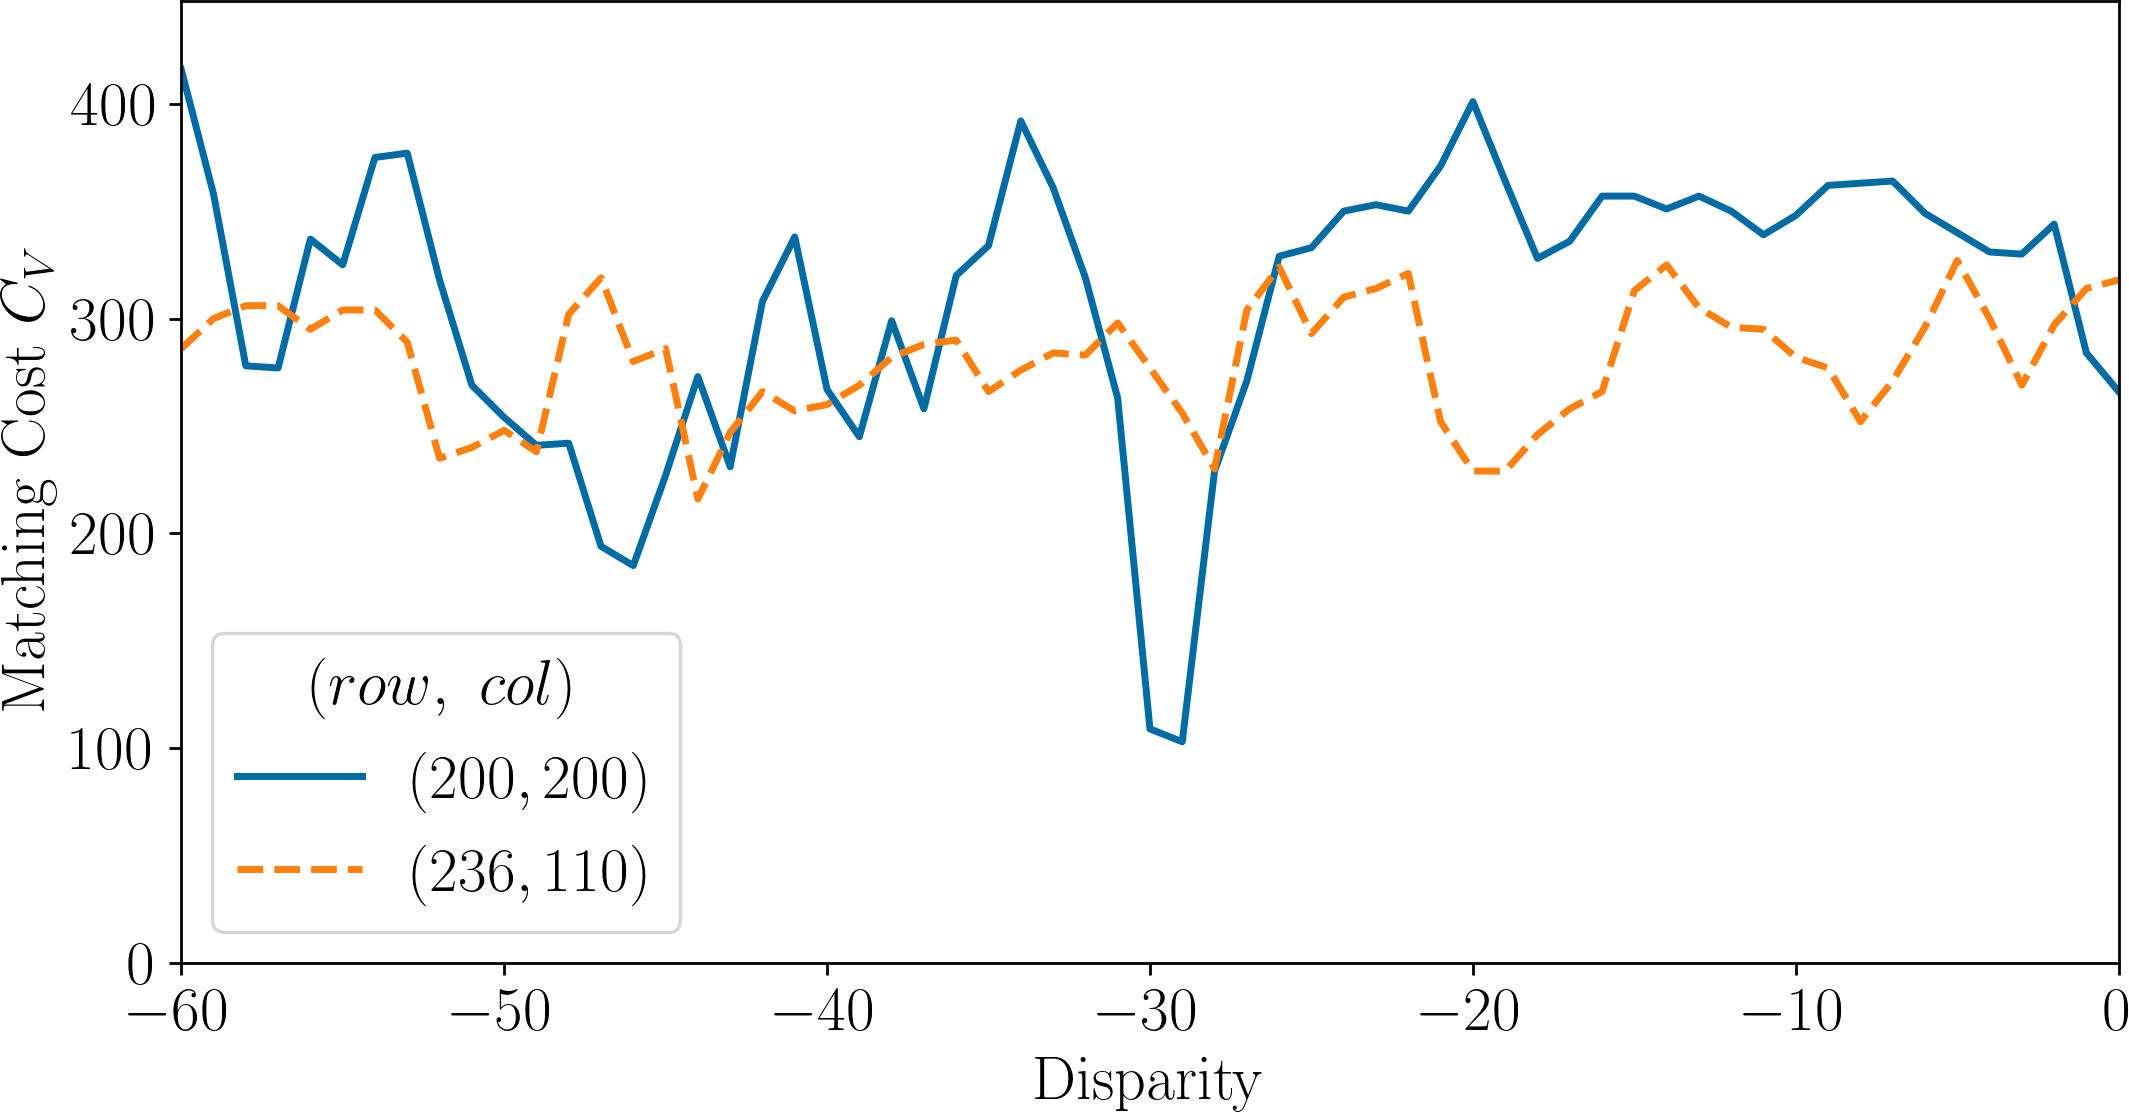
\includegraphics[width=\linewidth]{Images/Chap_5/cost_curve_not_normalized.png}
        \caption{Two cost curves}
        \label{fig:cost_curves_a}
    \end{subfigure}\hfill
    \begin{subfigure}[t]{0.47\linewidth}
        \centering
        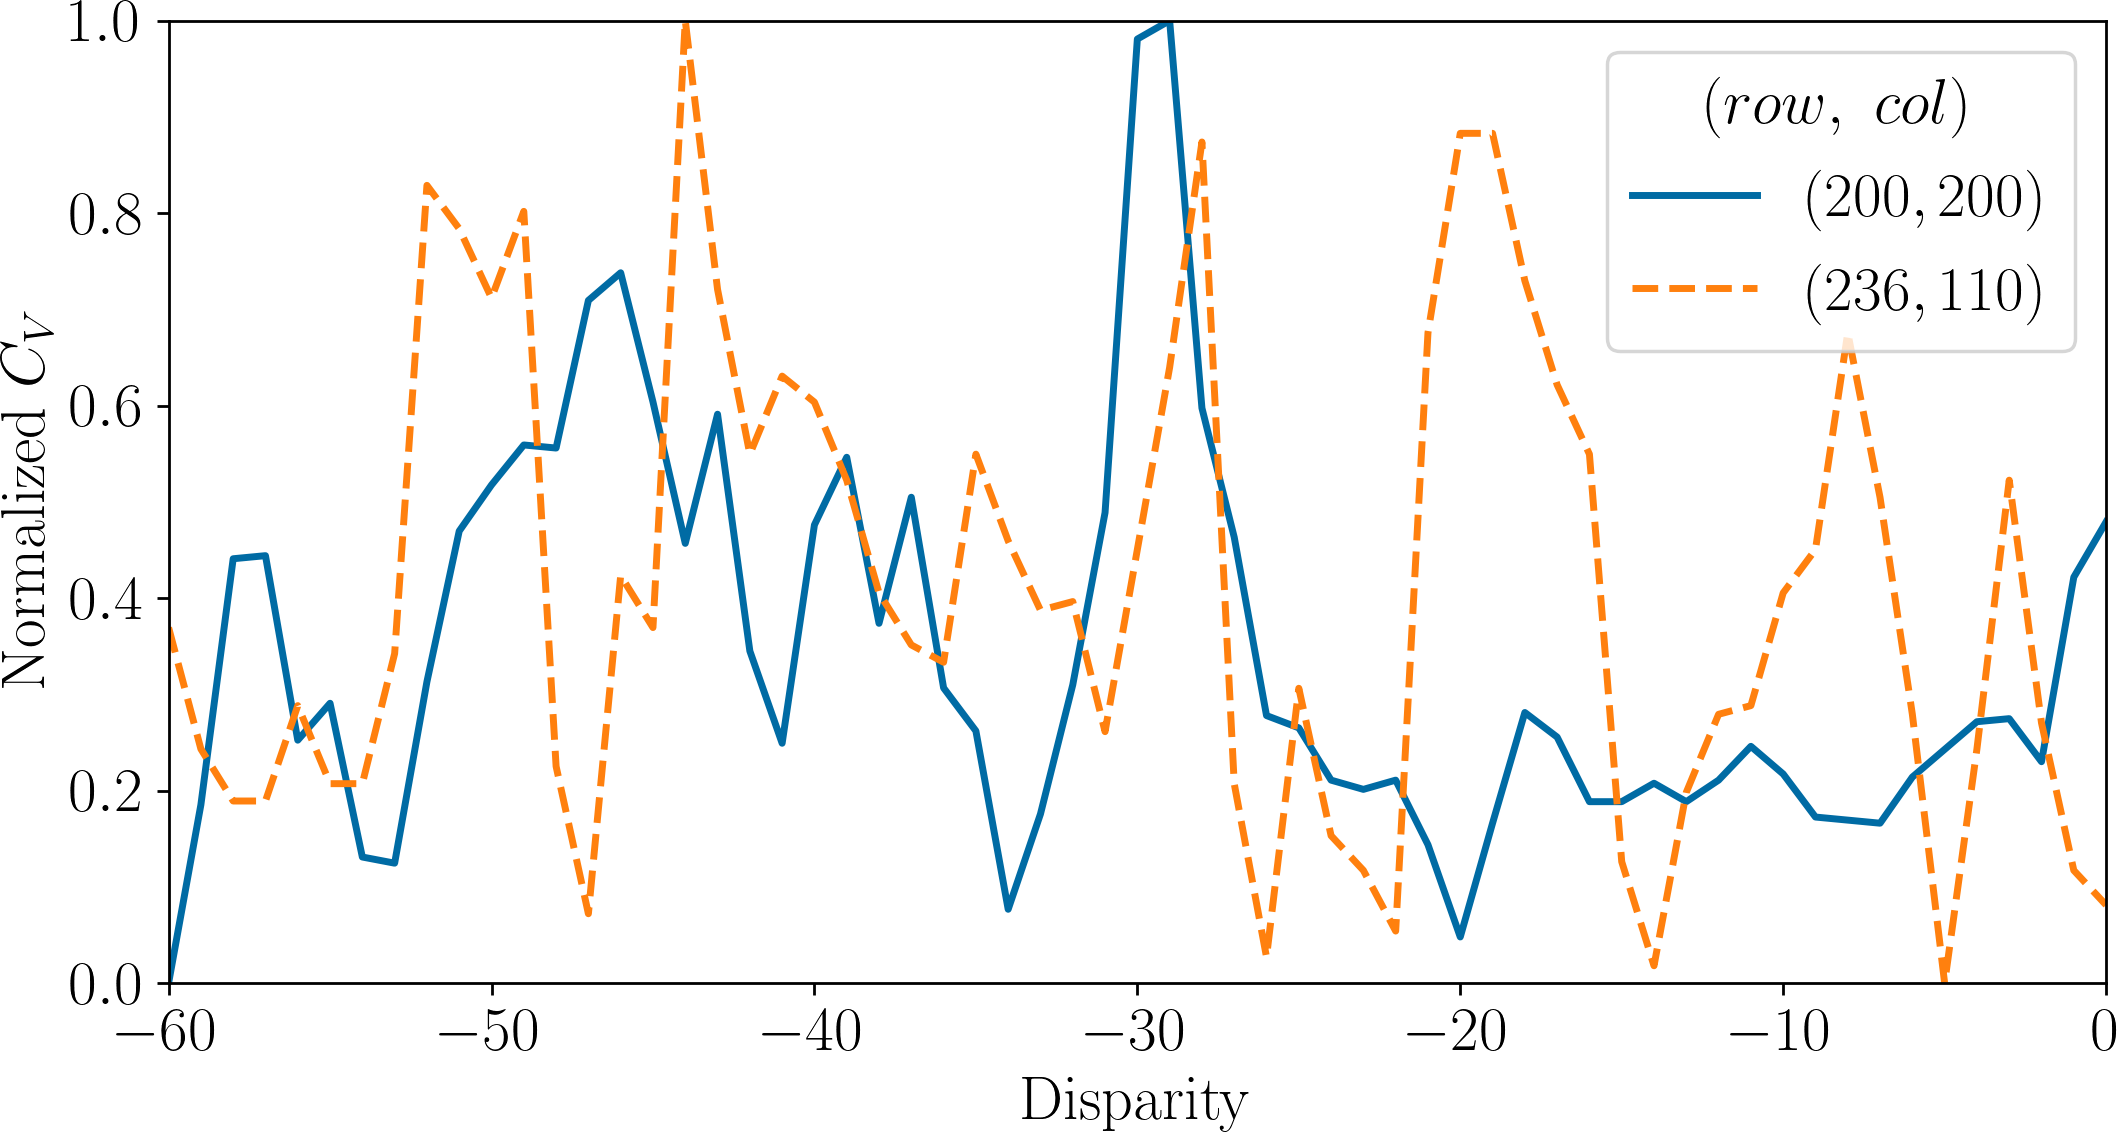
\includegraphics[width=\linewidth]{Images/Chap_5/cost_curve_bad_normalized.png}
        \caption{Normalized cost curves with local extrema}
        \label{fig:cost_curves_b}
    \end{subfigure}
    \begin{subfigure}[t]{0.47\linewidth}
        \centering
        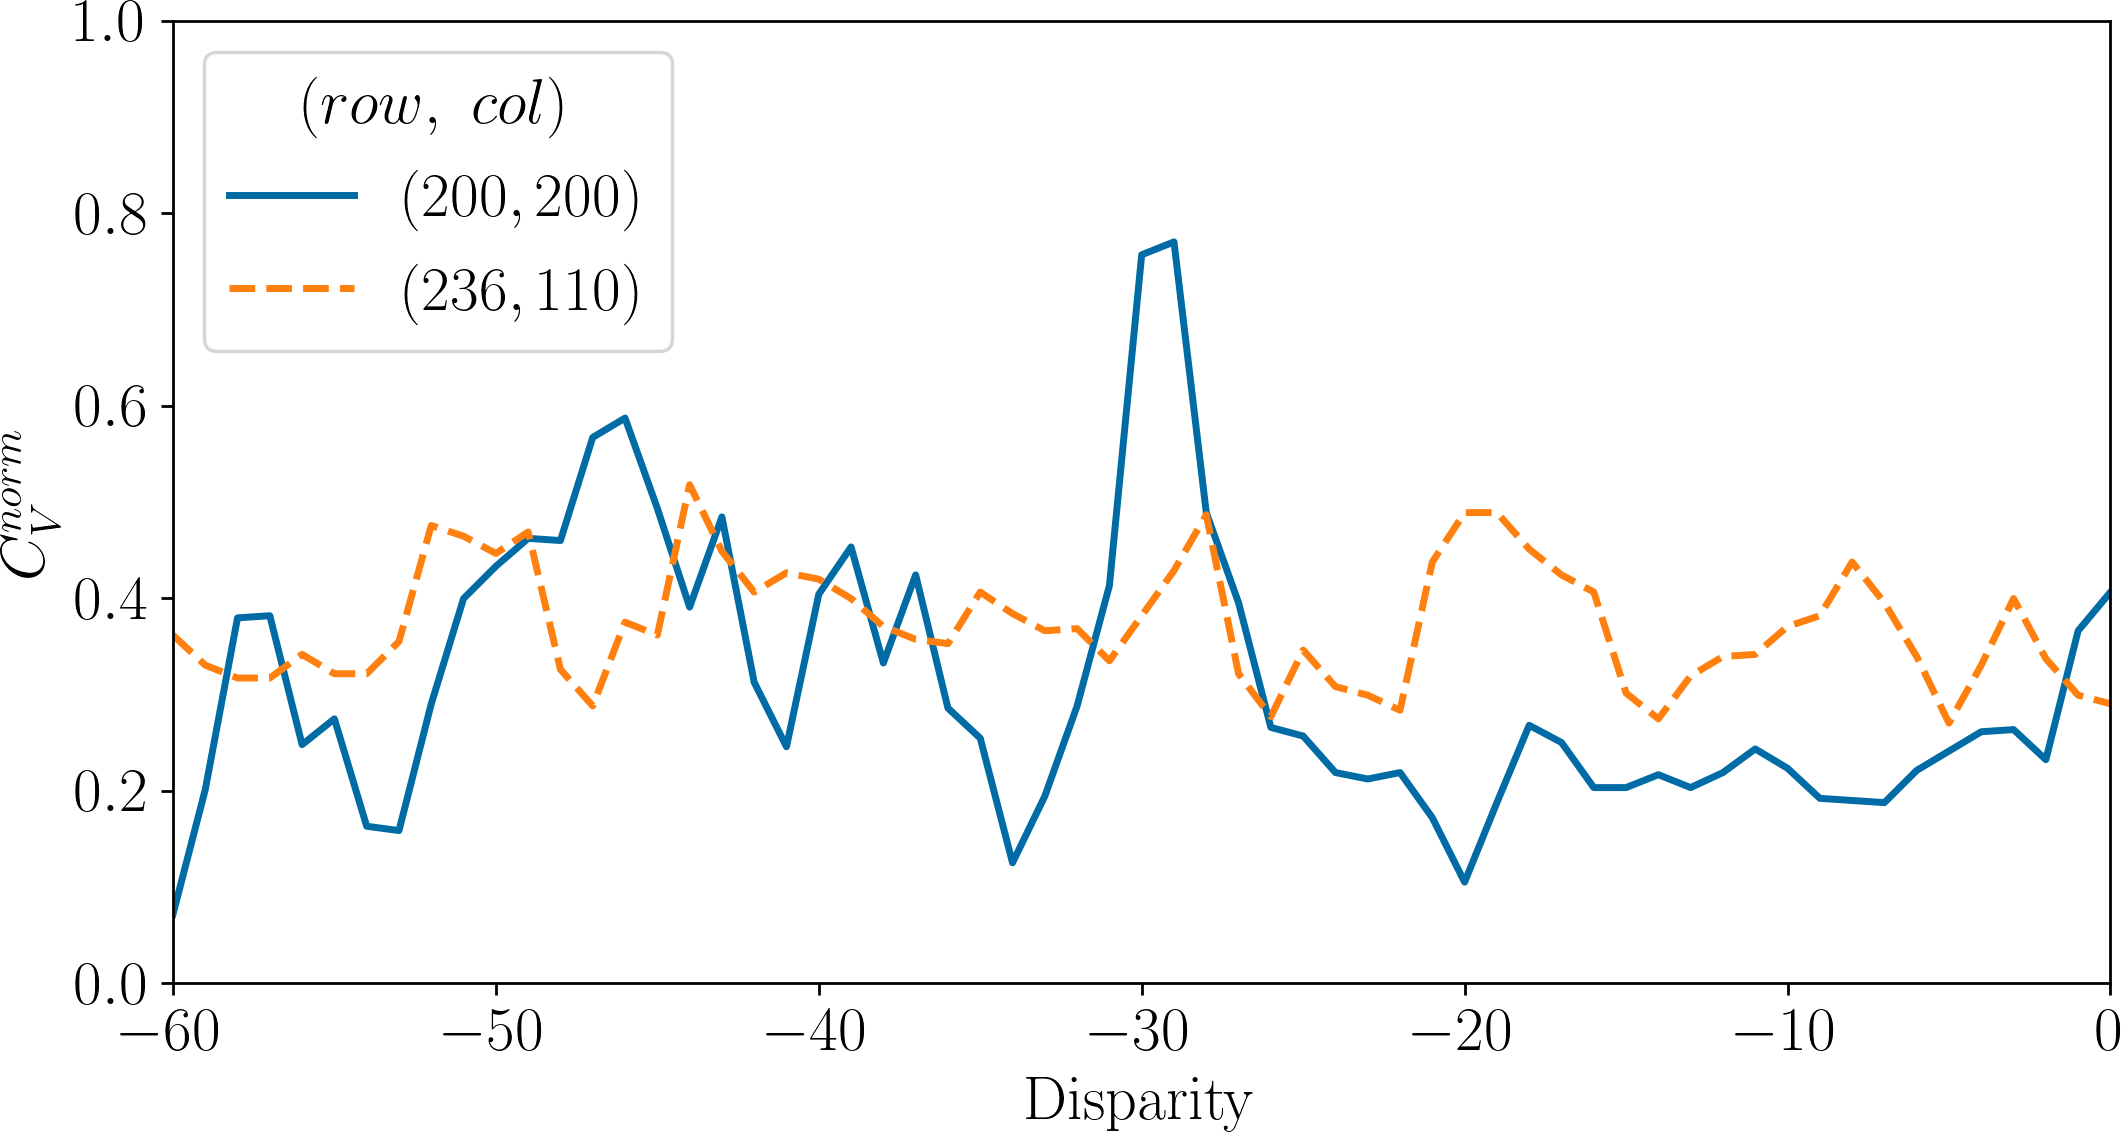
\includegraphics[width=\linewidth]{Images/Chap_5/cost_curve_normalized.png}
        \caption{Normalized cost curves $C_V^{norm}$ with global extrema}
        \label{fig:cost_curves_c}
    \end{subfigure}\hfill
    \begin{subfigure}[t]{0.47\linewidth}
        \centering
        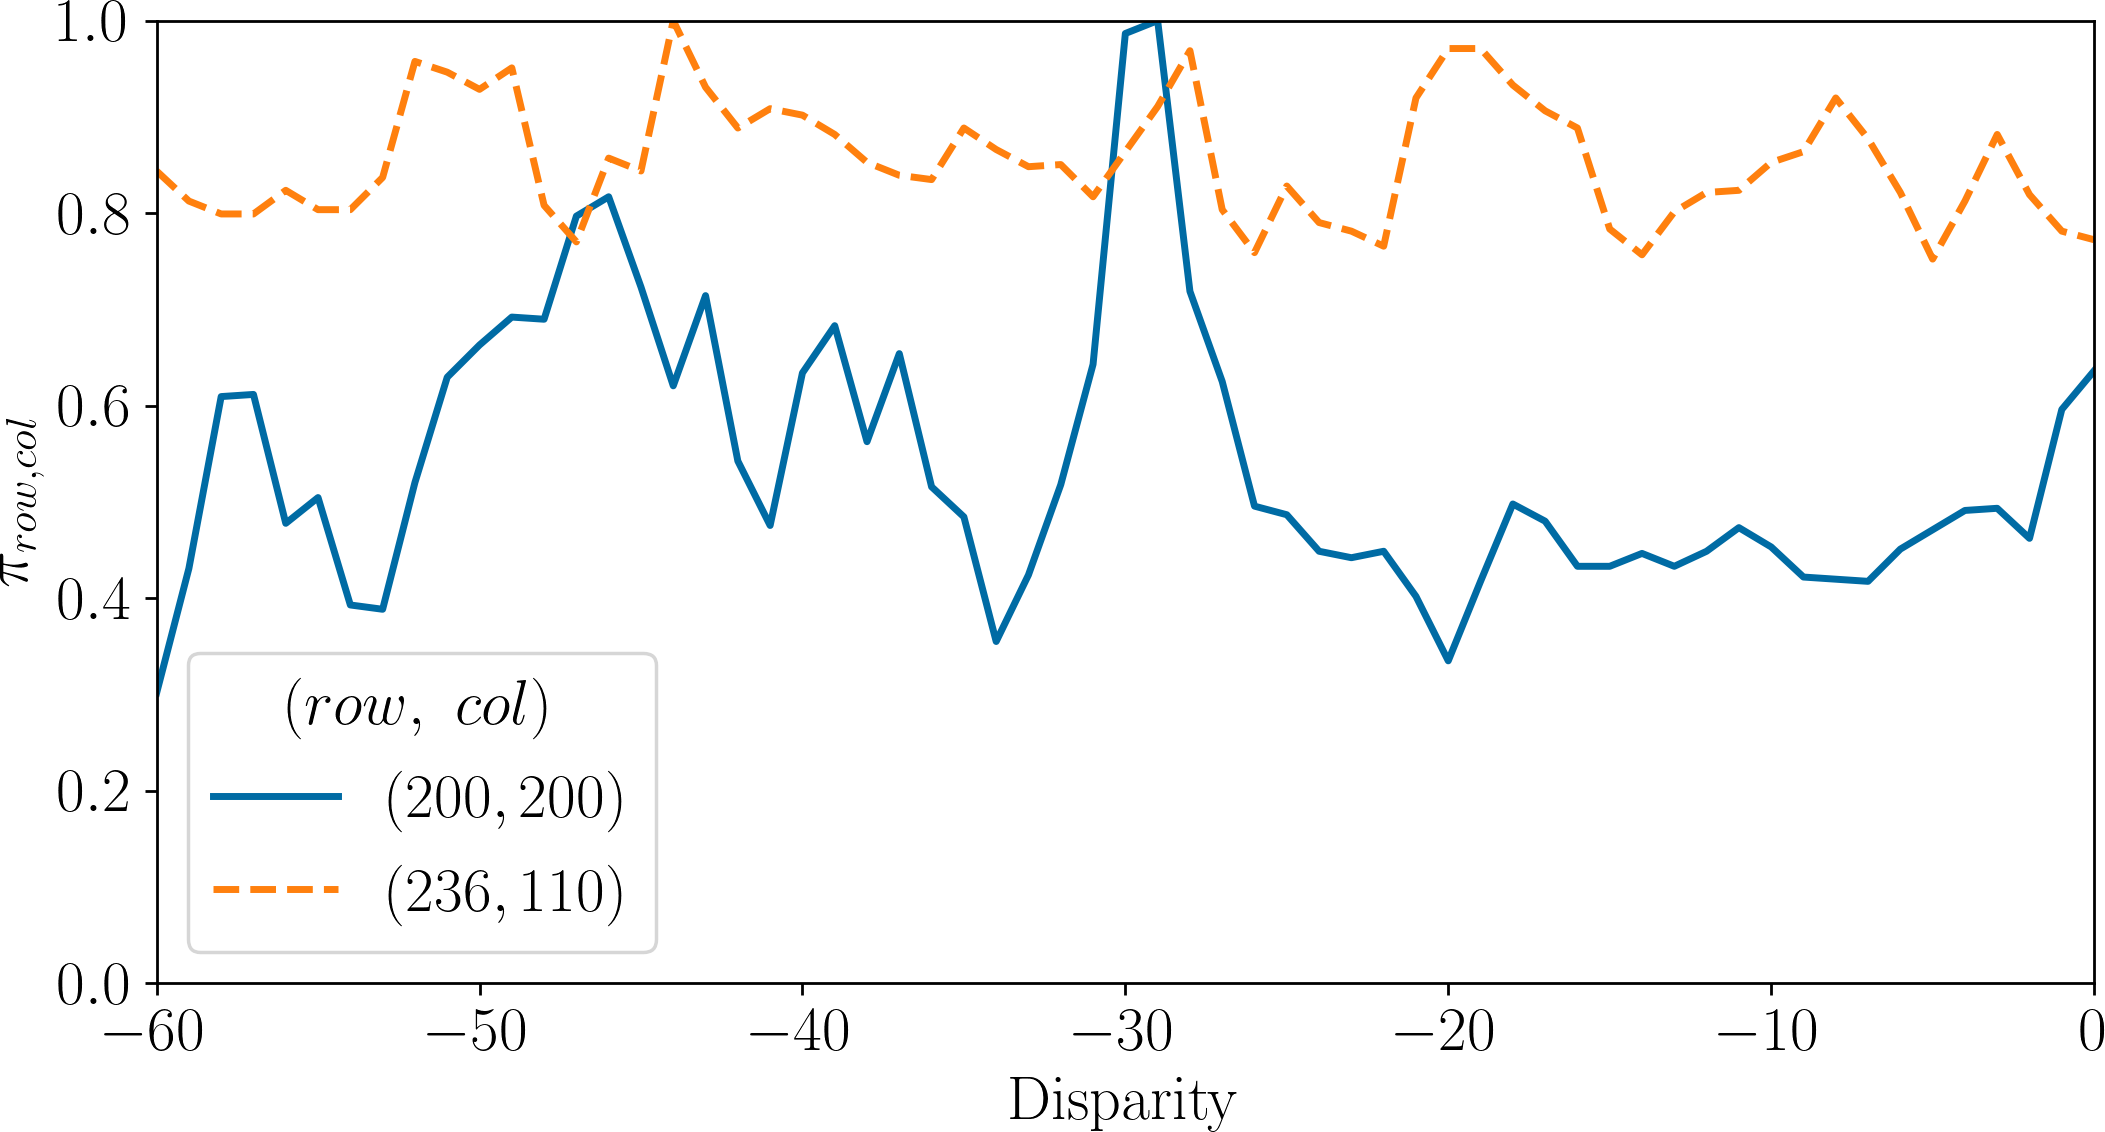
\includegraphics[width=\linewidth]{Images/Chap_5/cost_curve_possibility_distribution.png}
        \caption{Possibility distributions resulting from the cost curves}
        \label{fig:cost_curves_d}
    \end{subfigure}\hfill
    \caption{Transformation of cost curves (CENSUS + \acrshort{sgm} on Middlebury Cones) into possibility distributions. \subref{fig:cost_curves_a} represents two cost curves that are normalized differently in \subref{fig:cost_curves_b} and \subref{fig:cost_curves_c}. \subref{fig:cost_curves_d} uses the normalization of \subref{fig:cost_curves_c} to create possibility distributions.}
    \label{fig:cost_curves_to_possibility}
\end{figure}

As stated previously, global extrema in \Cref{eq:normalized_cost_curve} are employed to minimize the stretching effect when converting cost curves into possibility distributions. Alternatively, we also could have used the theoretical extrema of a cost curve instead. For instance, the CENSUS cost function on a $5\times5$ window provides values between $0$ and $C_{max}=24$. Adding \acrshort{sgm} regularization with penalty $P_2$ on $8$ directions yields cost volumes values between $0$ and $8\times(C_{max}+P_2)$ \cite{hirschmuller_accurate_2005}. However, this maximal cost is rarely attained in real case scenarios. Therefore, using theoretical extrema of the cost volume is too pessimistic and tends to over-compress the normalized cost curves. It is instead preferred to use global extrema of the cost volume for the normalization, as we assume the best and worst match should have similar cost values across different scenes. This hypothesis is not restrictive for the images we consider in our stereo matching problem, as the size and diversity inside each scene lead to similar extrema.  When processing very large images, the \acrshort{cars} stereo pipeline divides the image into small tiles that are processed in parallel. There is no guarantee that the cost volume extrema of each tile would be the same. In practice, cost volume extrema are similar for large images. We therefore assume differences in extrema are negligible.

\subsection{From Possibilities to Disparity Confidence Intervals}
With the possibility distributions defined, our next objective is to establish a set of most possible disparities. As presented previously, we decided to aim for sets containing the true disparity $90\%$ of the time. To define this set of most possible disparities, we compute the $\alpha$-cut from \Cref{def:alpha_cut}, or, in other words, the set of all disparities $D_\alpha$ whose possibility is greater than $\alpha$:
\begin{align}
    D_\alpha=\{~ d ~|~ \pi_{\rowcol}(d)\geqslant\alpha\}\label{eq:set_of_possible_disparities}
\end{align}
By looking at possibility distributions obtained from different cost curves for which we know the true disparity, we first fixed the value $\alpha$ at $0.9$. In depth study of this parameter will be conducted in \hyperref[chap:annex]{Annex}, in order to see if it depends on the cost function, the type of scene considered, and to provide general guidelines on its optimal value. In the following, when the value of $\alpha$ is not specified, it will always be set at $0.9$. \Cref{fig:disparity_intervals_a,fig:disparity_intervals_b} graphically represent $D_\alpha$ for the cost curves of \Cref{fig:cost_curves_to_possibility}.


\begin{remark}
    The fact that its value is the same as the $90\%$ confidence objective is a coincidence, and one should not assume that $\alpha$ and the confidence objective should be the same. Indeed, raising the $\alpha$ value would decrease the size of the set $D_\alpha$ and therefore decrease the proportion of sets containing the true disparity, \ie the global confidence rate of intervals.
\end{remark}

\begin{remark}
    We are modeling the epistemic uncertainty of the cost curves using possibility distributions. In the rest of this chapter, we use a possibility distribution for each cost curve because we think it is a correct model in itself for the uncertainty we encounter. It is however possible to have a probabilistic interpretation of possibilities.
    
    We saw in \Cref{eq:credal_set_possibility} from \Cref{chap:representation_of_uncertainty} that one way of interpreting $\pi_{\rowcol}$ is that it defines a set of probability distributions, \ie a credal set $\M$. We can also define $D_\alpha$ using this set $\M$, as:
    \begin{align}
        D_\alpha=\{~ d ~|~ \exists P\in\M ~\st~ P(d)\geqslant \alpha\}
    \end{align}
    or in plain words, $D_\alpha$ is the set of all disparities $d$ for which there exists a probability in $\M$ whose value is greater than $\alpha$ for $d$. We will not rely on this interpretation in the rest of this chapter, and instead only reason in terms of possibilities.
\end{remark}

\Cref{eq:set_of_possible_disparities} defines a set of disparities $D_\alpha$ that is not necessarily convex. We will rather consider disparity confidence intervals $I_\alpha$ deduced from $D_\alpha$ in the rest of this chapter:
\begin{align}
    I_\alpha = [\underline{I}_\alpha,~\overline{I}_\alpha]=[\min D_\alpha, ~\max D_\alpha]\label{eq:confidence_disparity_intervals}
\end{align}
\Cref{fig:disparity_intervals_c,fig:disparity_intervals_d} graphically represent how $I_\alpha$ is determined for the two possibility distributions of the cost curves in \Cref{fig:cost_curves_to_possibility}. In the rest of this section, we will not make any distinction between disparity confidence intervals, disparity intervals, confidence intervals or simply intervals. A disparity interval is the convex envelope of its disparity set $D_\alpha$, which is a conservative approach as observed in \Cref{fig:disparity_intervals_b,fig:disparity_intervals_d}.

Considering intervals thus presents the advantage of working with convex sets and only requiring two scalars to describe the set. Users of \acrshort{dsm}s produced by stereophotogrammetry are familiar with confidence intervals \cite{oksanen_digital_2006, wang_robust_2015, panagiotakis_validation_2018, deschamps-berger_apport_2021, hugonnet_uncertainty_2022}. It will also facilitate further processing in the rest of the stereo pipeline, as we only need to take into account $2$ bounds to characterize possible disparities, instead of sets of arbitrary shape.
\begin{figure}
    \centering
    \begin{subfigure}[t]{0.47\linewidth}
        \centering
        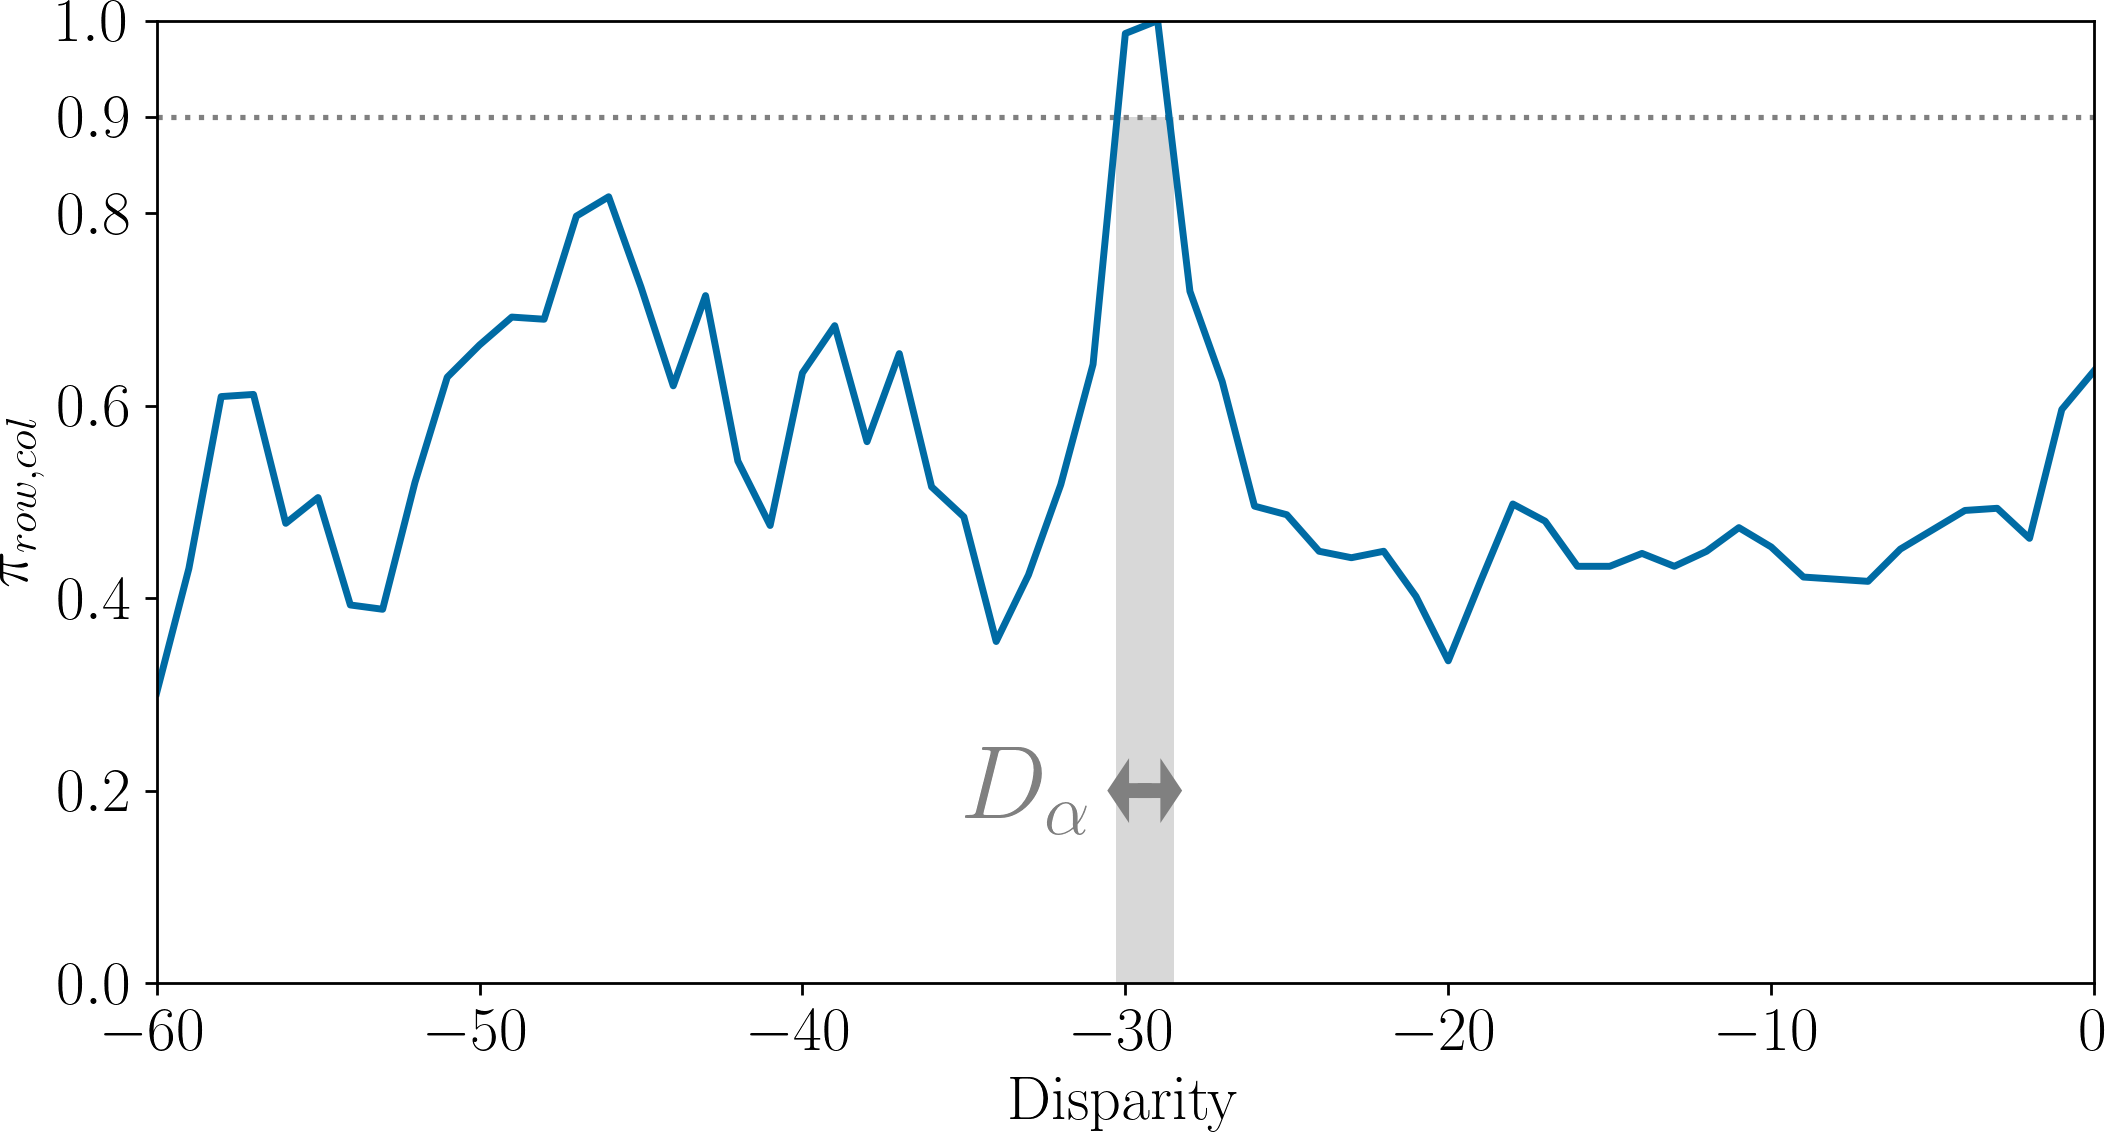
\includegraphics[width=\linewidth]{Images/Chap_5/disparity_interval_1.png}
        \caption{$D_\alpha$ for the blue possibility of \Cref{fig:cost_curves_d}}
        \label{fig:disparity_intervals_a}
    \end{subfigure}\hfill
    \begin{subfigure}[t]{0.47\linewidth}
        \centering
        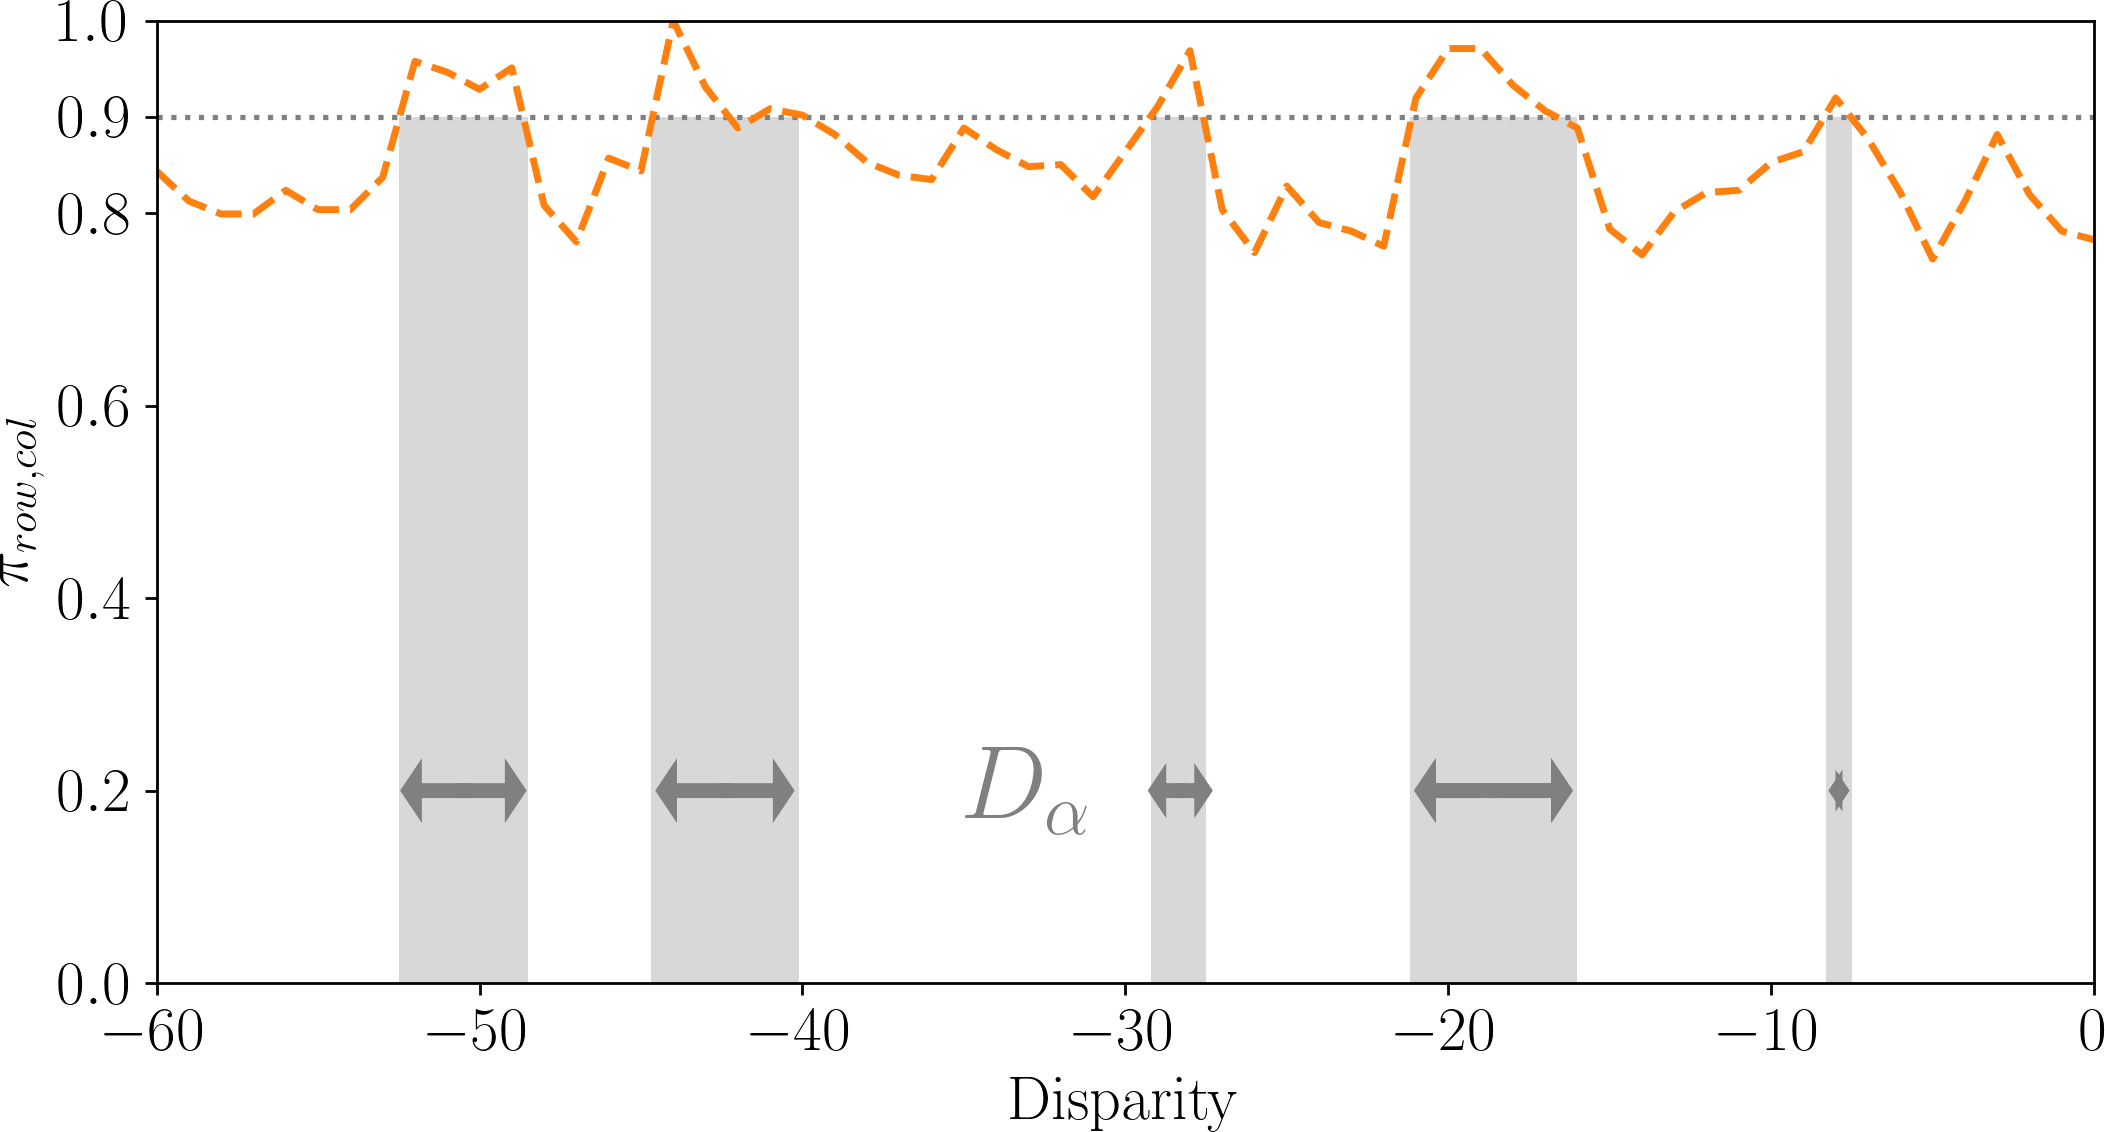
\includegraphics[width=\linewidth]{Images/Chap_5/disparity_interval_2.png}
        \caption{$D_\alpha$ for the orange possibility of \Cref{fig:cost_curves_d}}
        \label{fig:disparity_intervals_b}
    \end{subfigure}
    \begin{subfigure}[t]{0.47\linewidth}
        \centering
        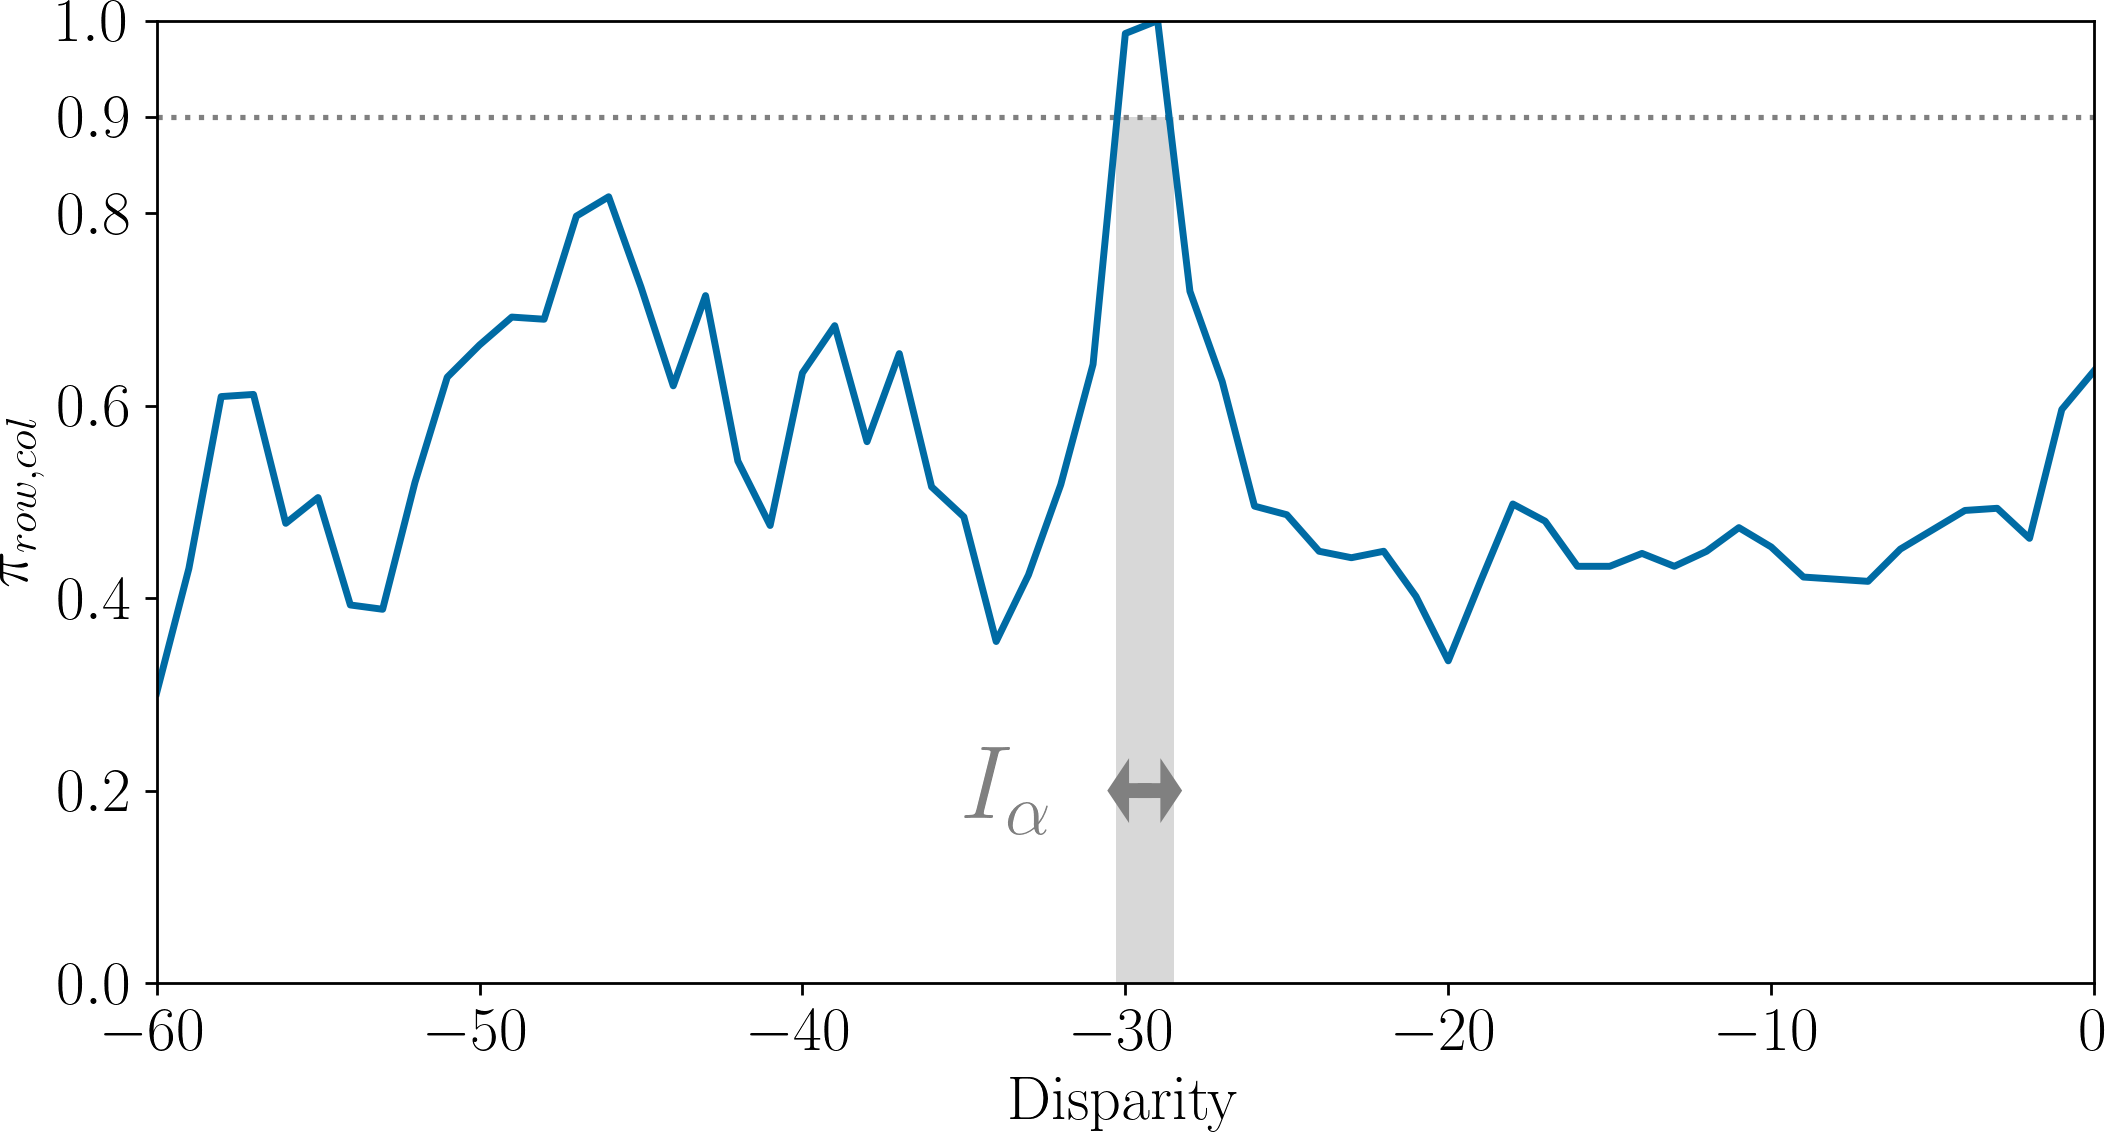
\includegraphics[width=\linewidth]{Images/Chap_5/disparity_interval_3.png}
        \caption{$I_\alpha$ for the blue possibility of \Cref{fig:cost_curves_d}}
        \label{fig:disparity_intervals_c}
    \end{subfigure}\hfill
    \begin{subfigure}[t]{0.47\linewidth}
        \centering
        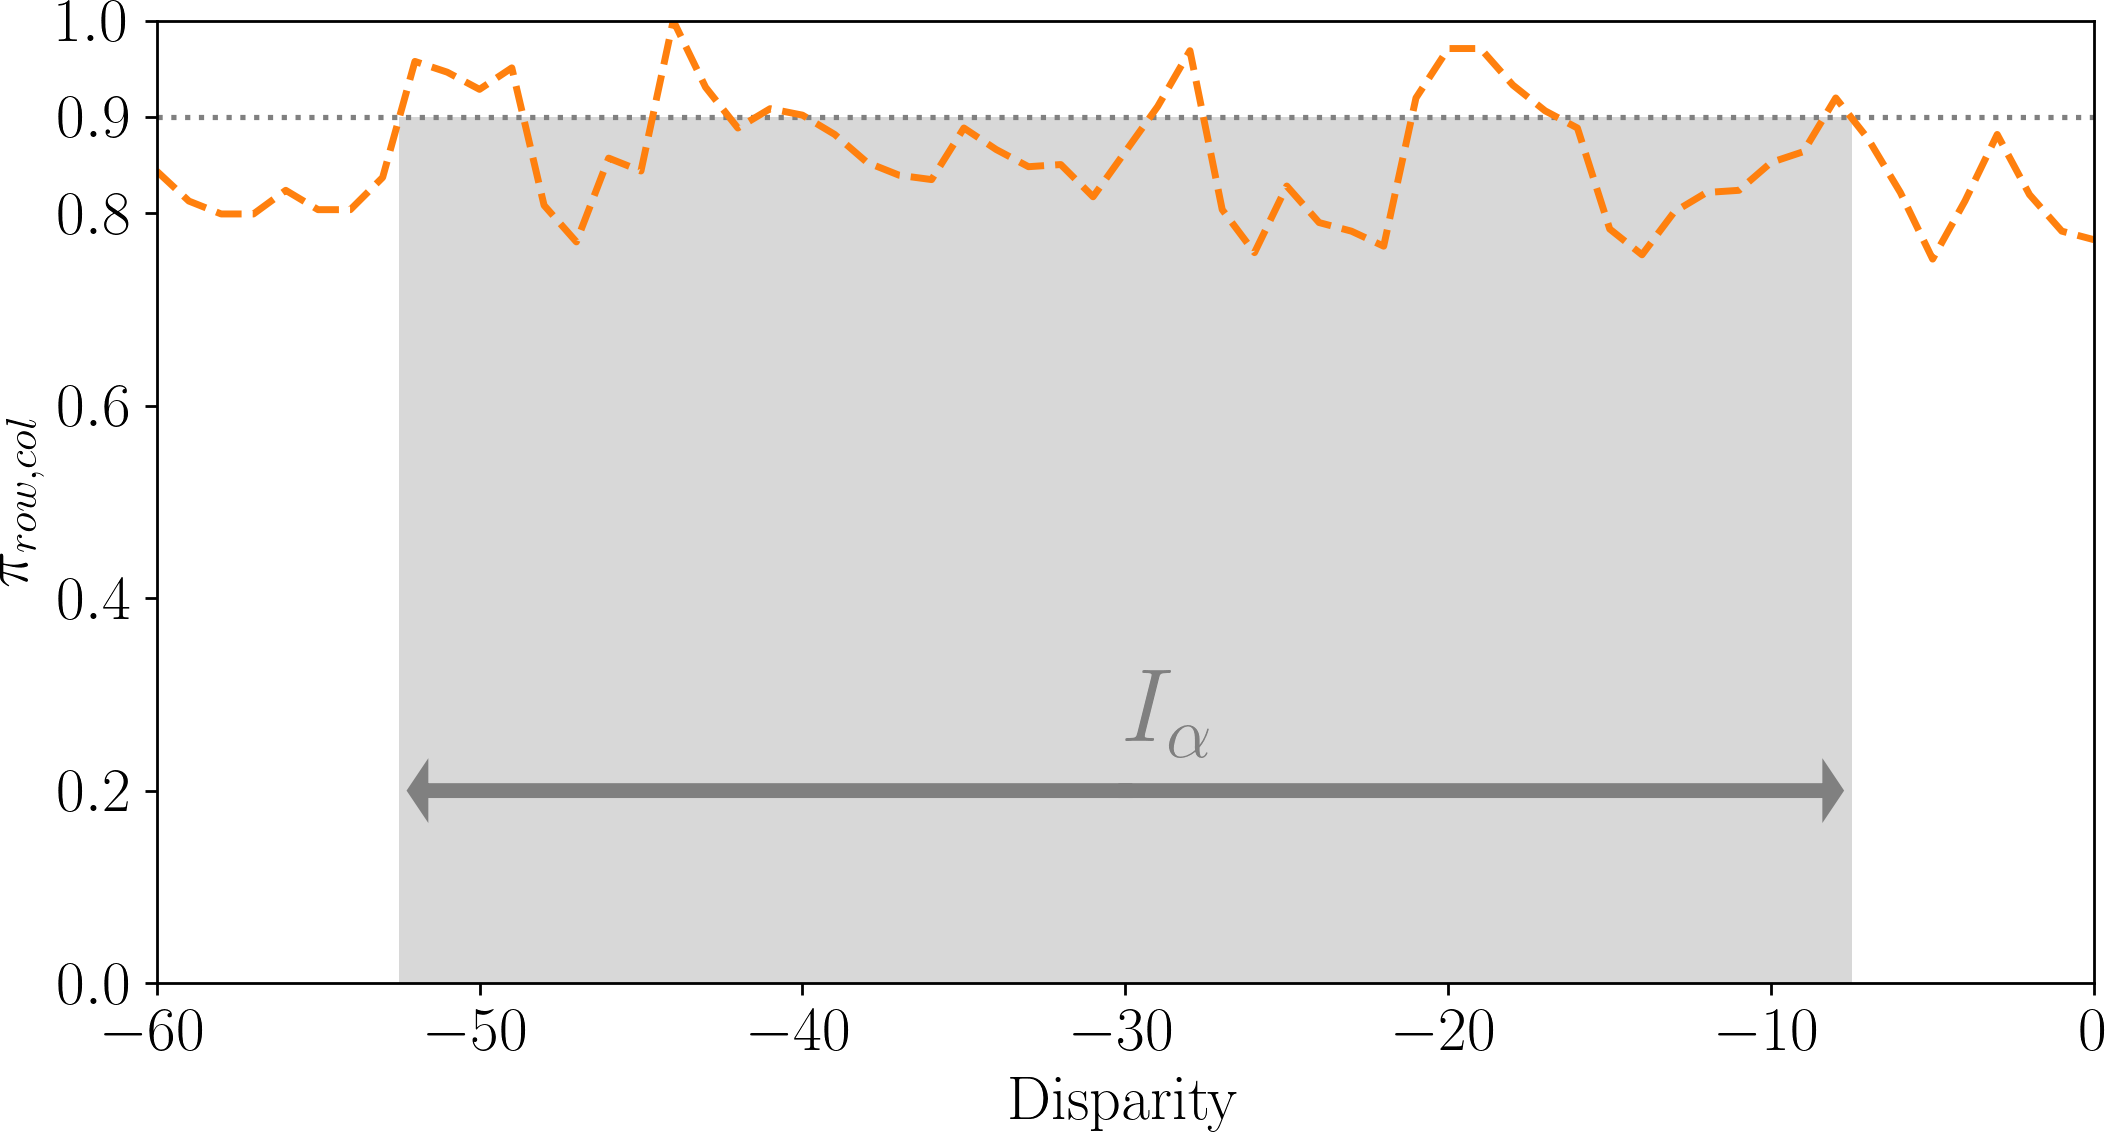
\includegraphics[width=\linewidth]{Images/Chap_5/disparity_interval_4.png}
        \caption{$I_\alpha$ for the orange possibility of \Cref{fig:cost_curves_d}}
        \label{fig:disparity_intervals_d}
    \end{subfigure}\hfill
    \caption{Set of possible disparities $D_\alpha$ and disparity intervals $I_\alpha$ with the same cost curves as in \Cref{fig:cost_curves_to_possibility}, with $\alpha=0.9$. \subref{fig:disparity_intervals_a} and \subref{fig:disparity_intervals_b} represent the set of possible disparities $D_\alpha$ from \Cref{eq:set_of_possible_disparities} in gray. \subref{fig:disparity_intervals_c} and \subref{fig:disparity_intervals_d} represent disparity intervals $I_\alpha$ from \Cref{eq:confidence_disparity_intervals} in gray. There is no difference between $D_\alpha$ and $I_\alpha$ for the blue curve, contrary to the orange dashed curve.}
    \label{fig:disparity_sets_and_intervals}
\end{figure}

\begin{figure}
    \centering
    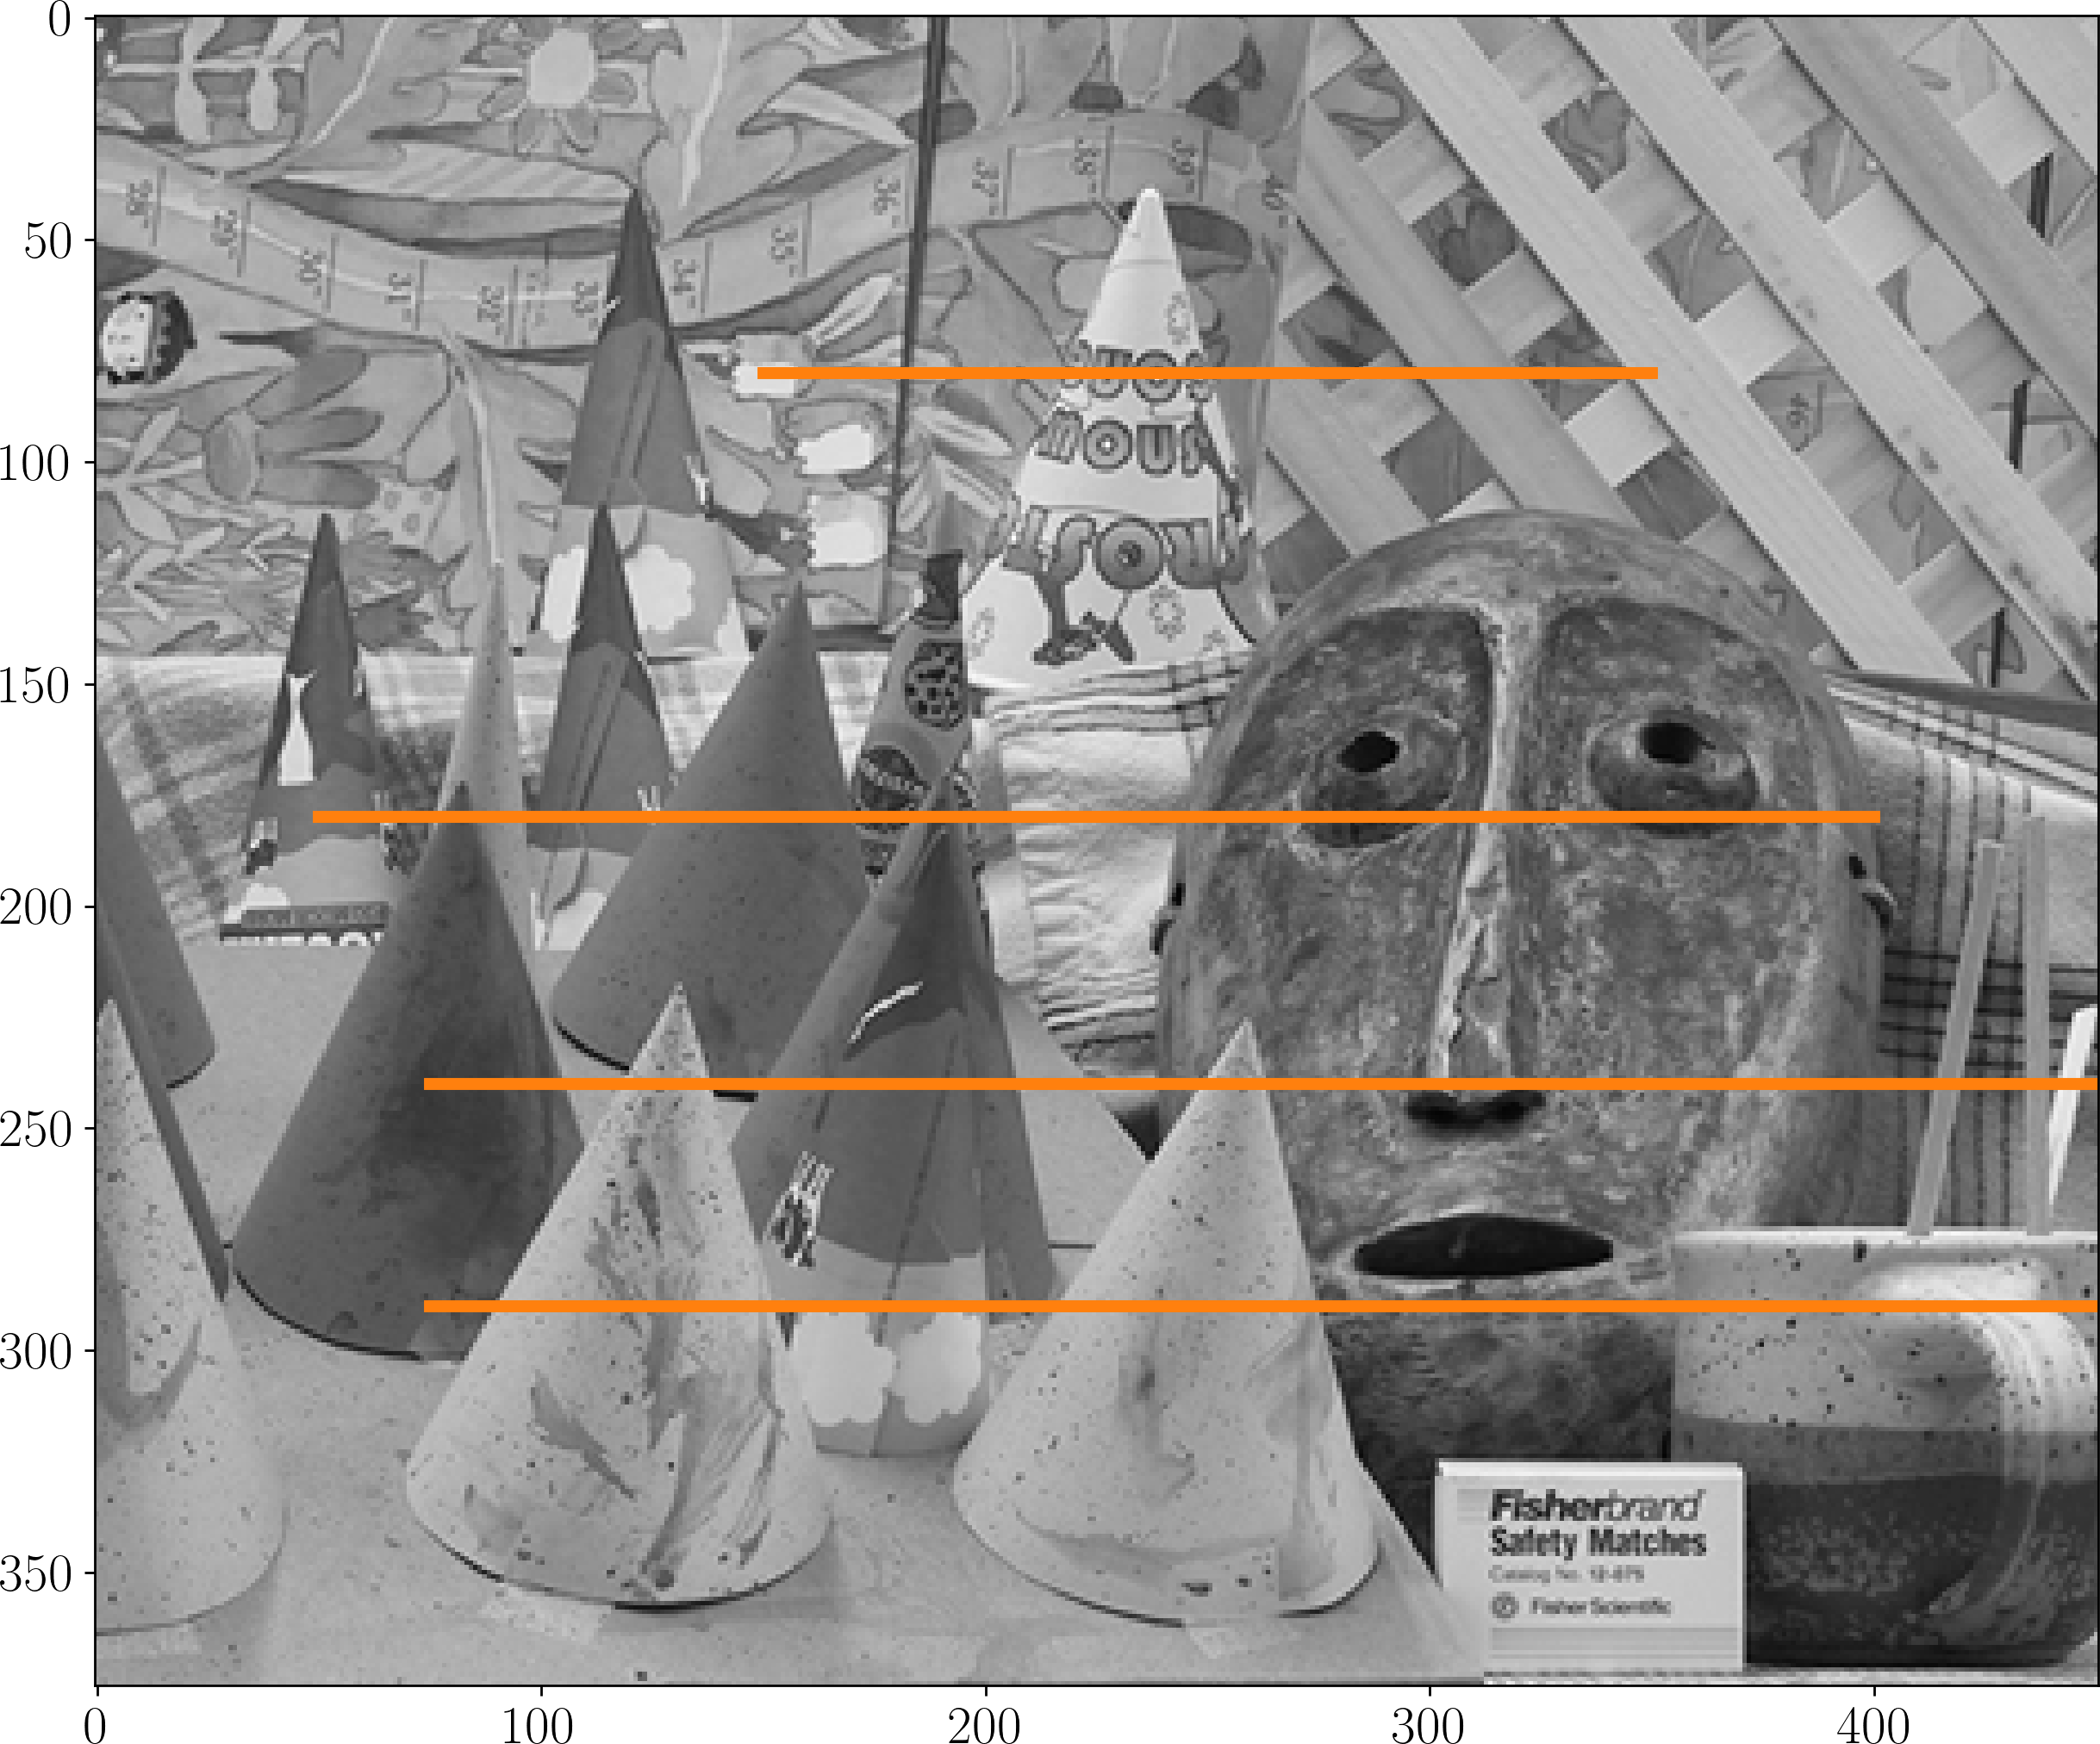
\includegraphics[width=0.5\linewidth]{Images/Chap_5/cones_with_rows.png}
    \caption{Left stereo image from Middlebury Cones. Disparity intervals $I_\alpha$ along orange lines are detailed in \Cref{fig:intervals_ambiguous_row_80_180,fig:intervals_ambiguous_row_240_290,fig:intervals_ambiguous_row_80,fig:intervals_ambiguous_row_180,fig:intervals_ambiguous_row_240,fig:intervals_ambiguous_row_290}}
    \label{fig:cones_with_rows}
\end{figure}

To qualitatively evaluate the behavior of disparity confidence intervals $I_\alpha$, we will look at their values for consecutive pixels of the same row. Rows selected for this analysis are presented in \Cref{fig:cones_with_rows}: the upper row ($80$) is smaller than the others, so more details can be observed, while other rows allows for a broader view of the intervals. We selected rows containing different disparity configurations in different part of the image, as adjacent rows tend to look relatively similar.

\begin{figure}
    \centering
    \begin{subfigure}[t]{\linewidth}
        \centering
        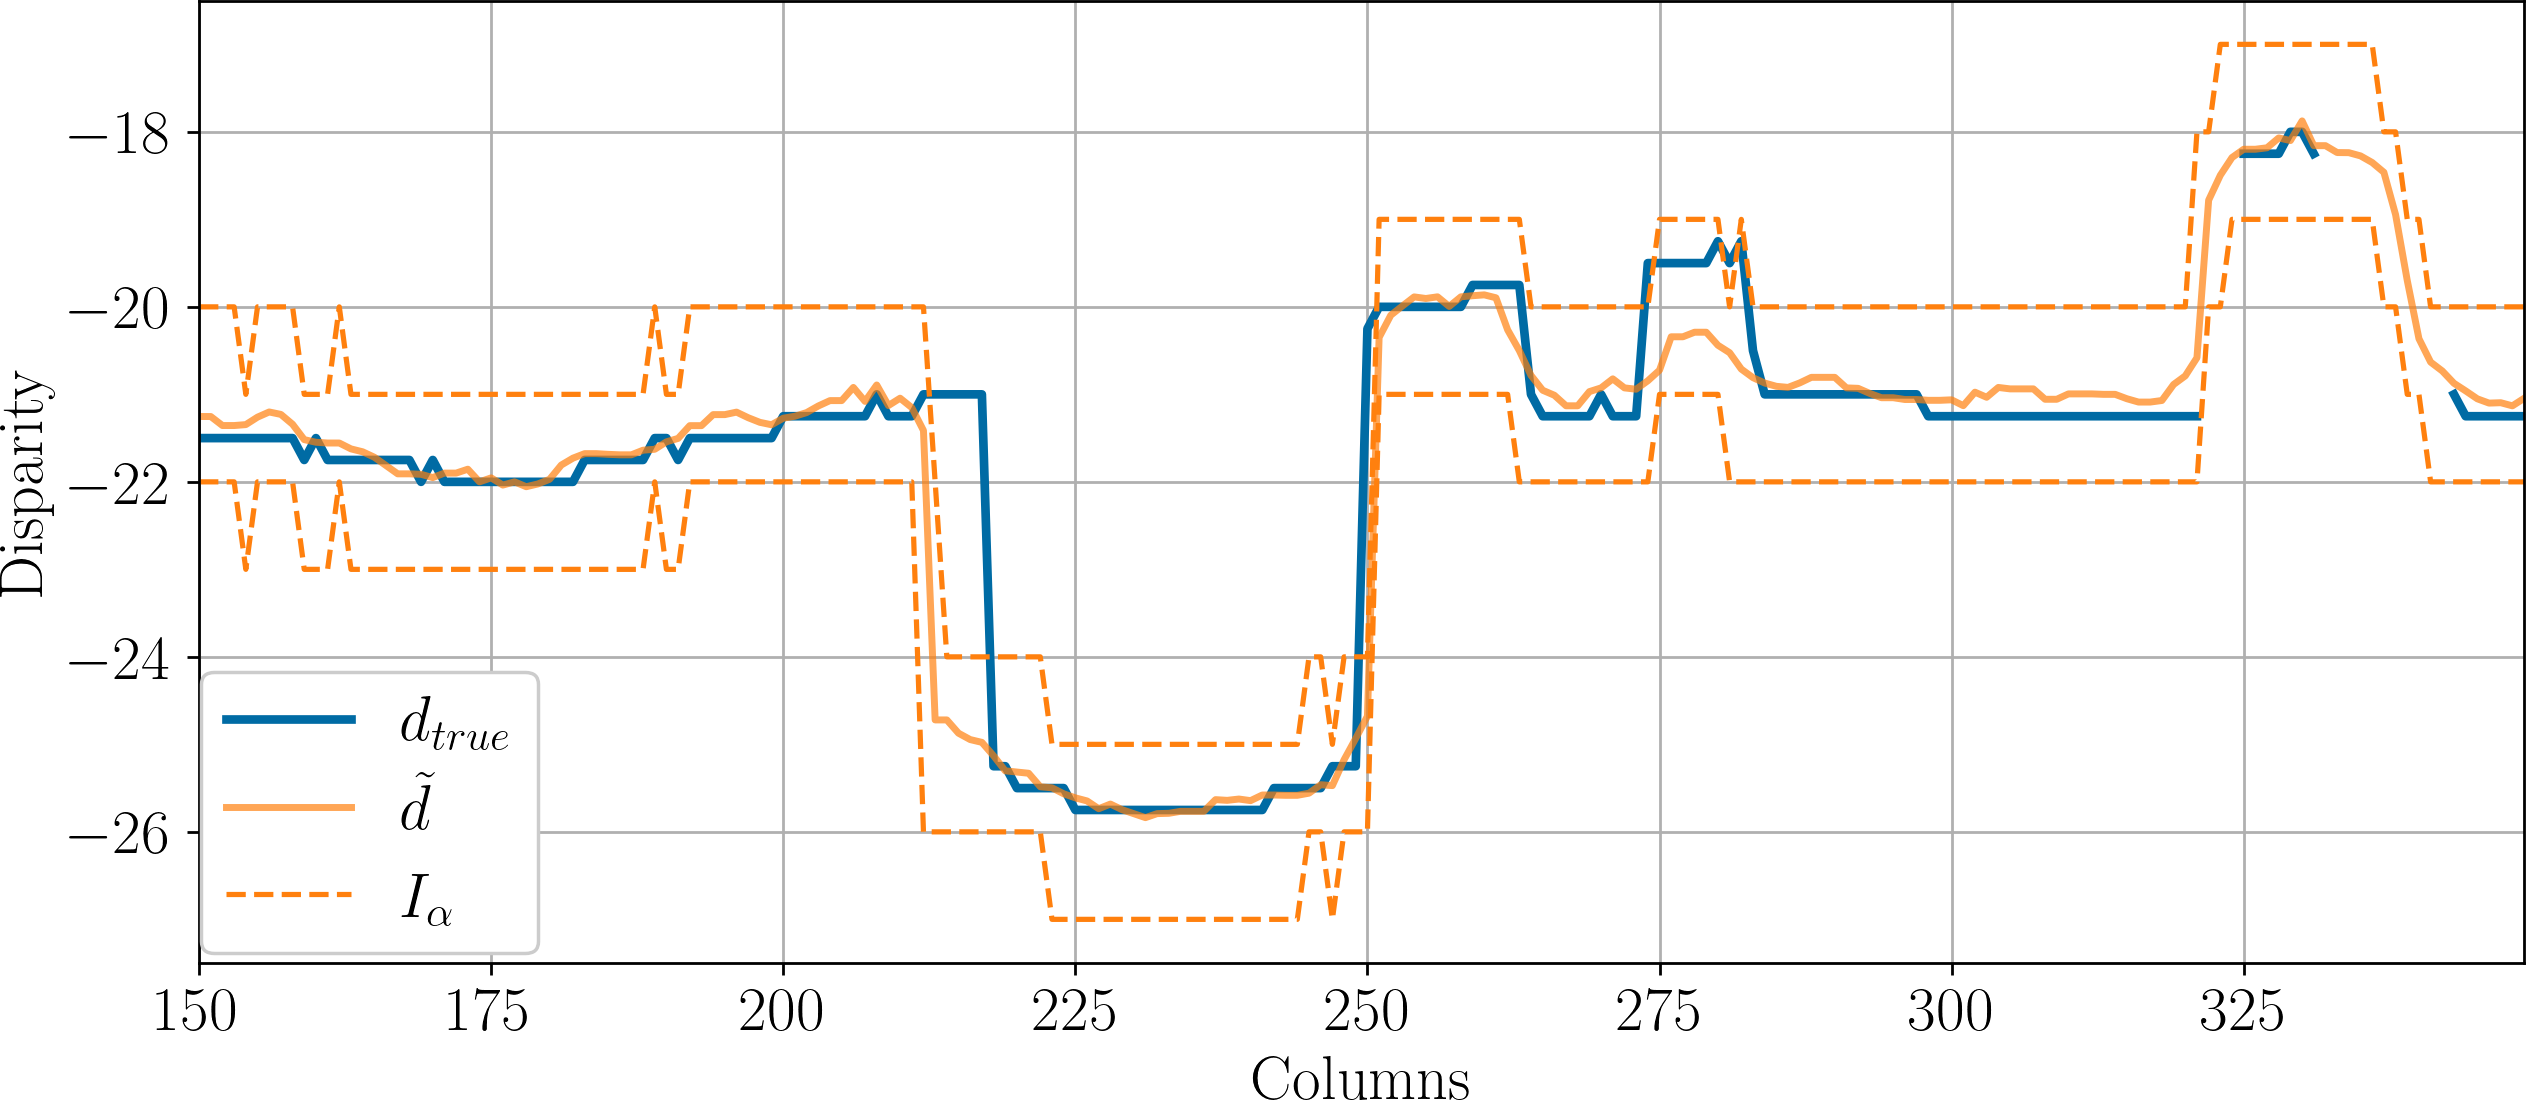
\includegraphics[width=\linewidth]{Images/Chap_5/intervals_ambiguous_area_row_80_1.png}
        \caption{$I_\alpha$ along row $80$}
        \label{fig:intervals_ambiguous_row_80_no_reg}
    \end{subfigure}\hfill
    \begin{subfigure}[t]{\linewidth}
        \centering
        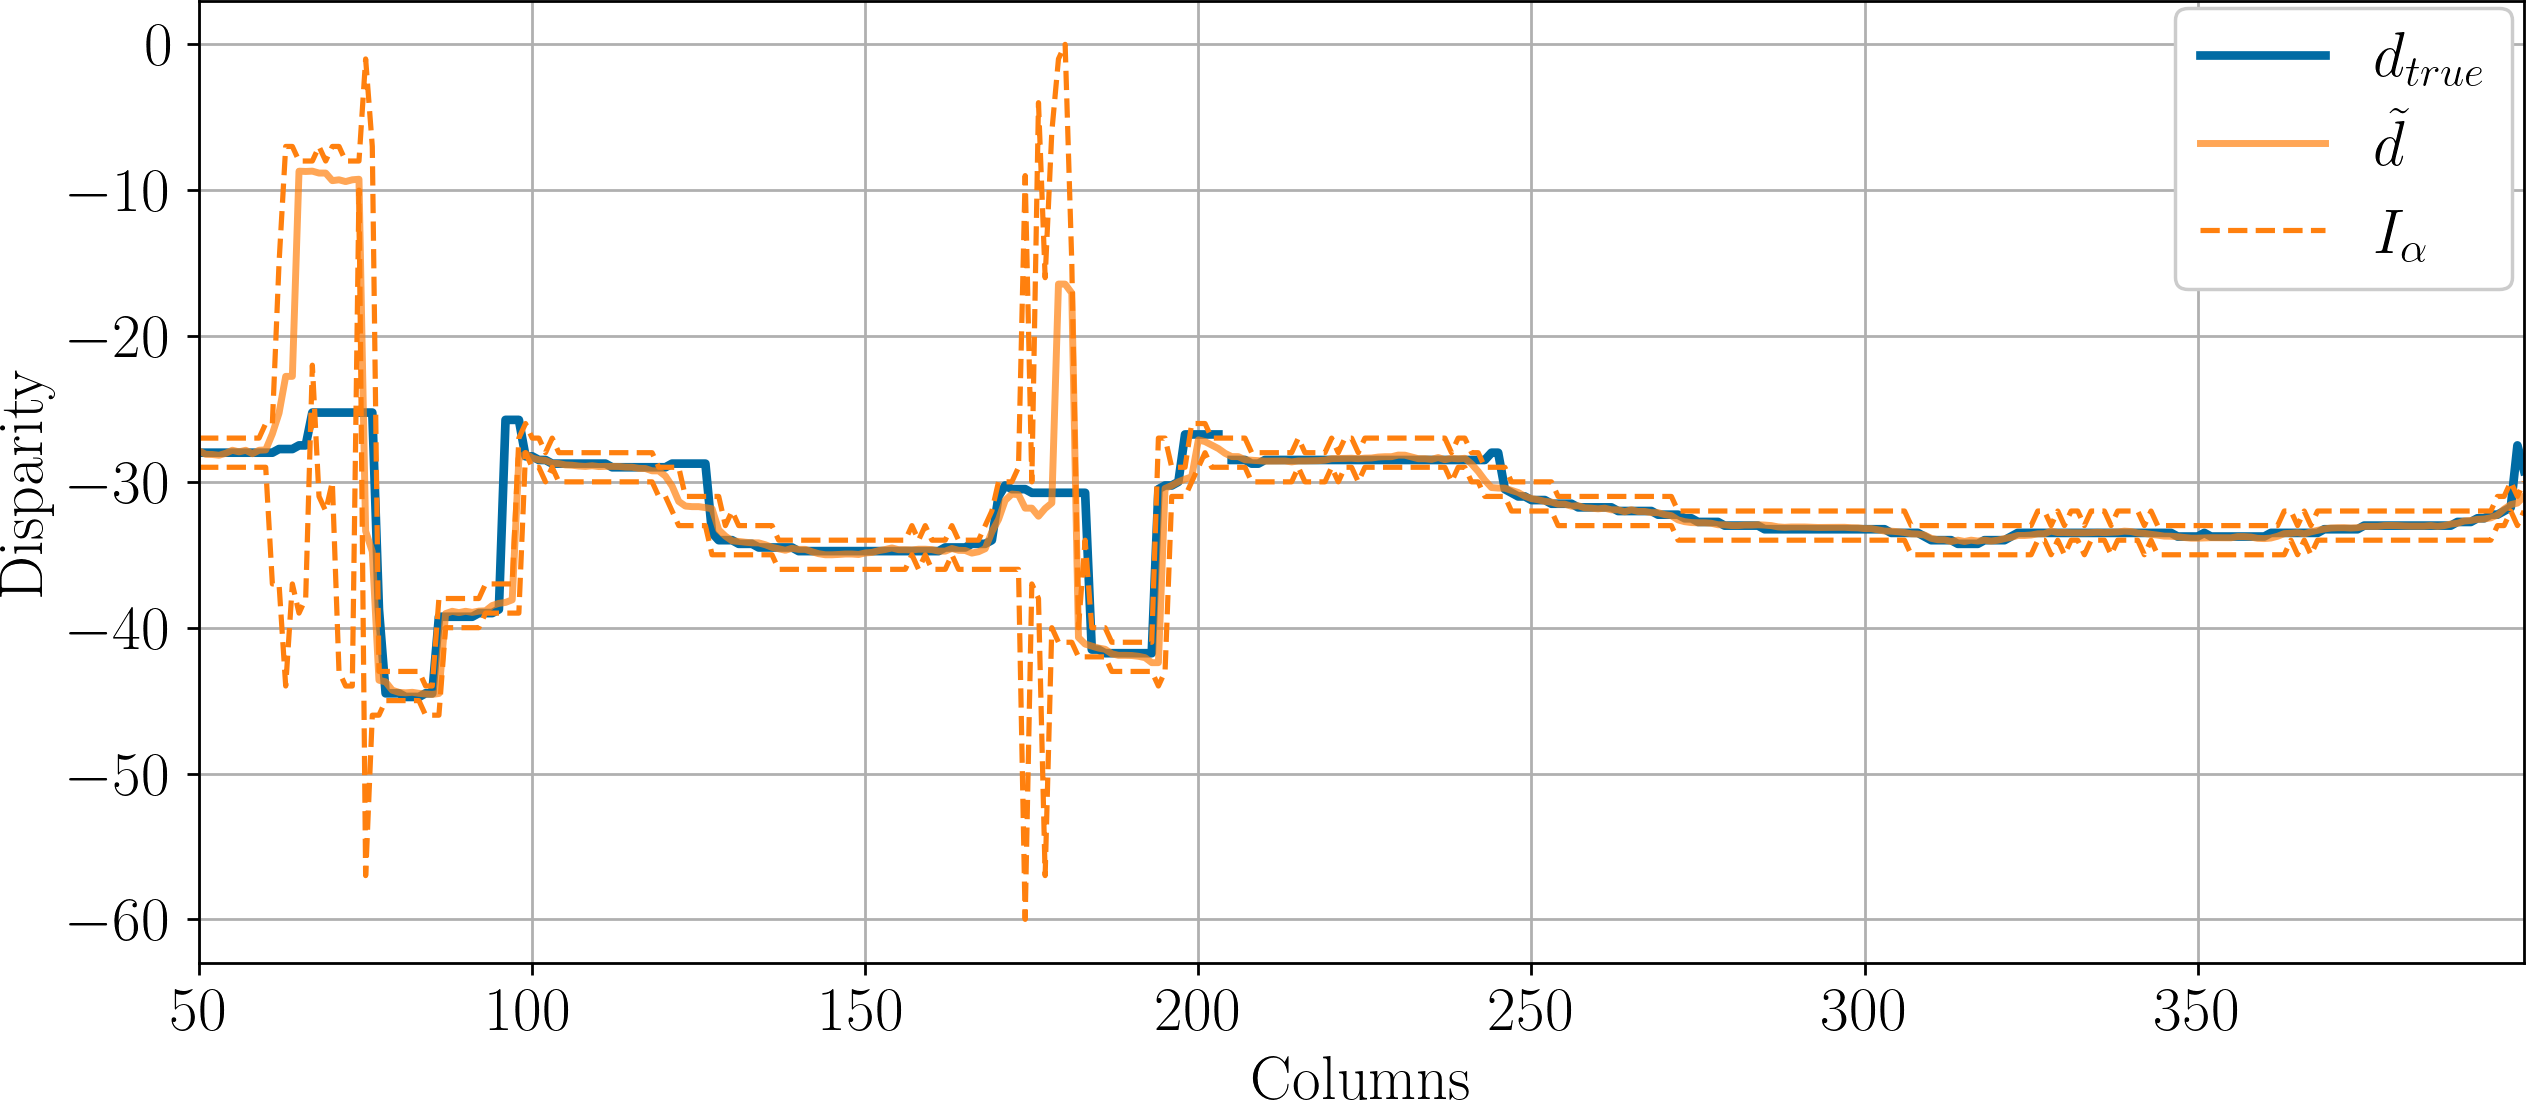
\includegraphics[width=\linewidth]{Images/Chap_5/intervals_ambiguous_area_row_180_1.png}
        \caption{$I_\alpha$ along row $180$}
        \label{fig:intervals_ambiguous_row_180_no_reg}
    \end{subfigure}
    \caption{$I_\alpha$ for the two top rows highlighted in \Cref{fig:cones_with_rows}}
    \label{fig:intervals_ambiguous_row_80_180}
\end{figure}

\begin{figure}
    \centering
    \begin{subfigure}[t]{\linewidth}
        \centering
        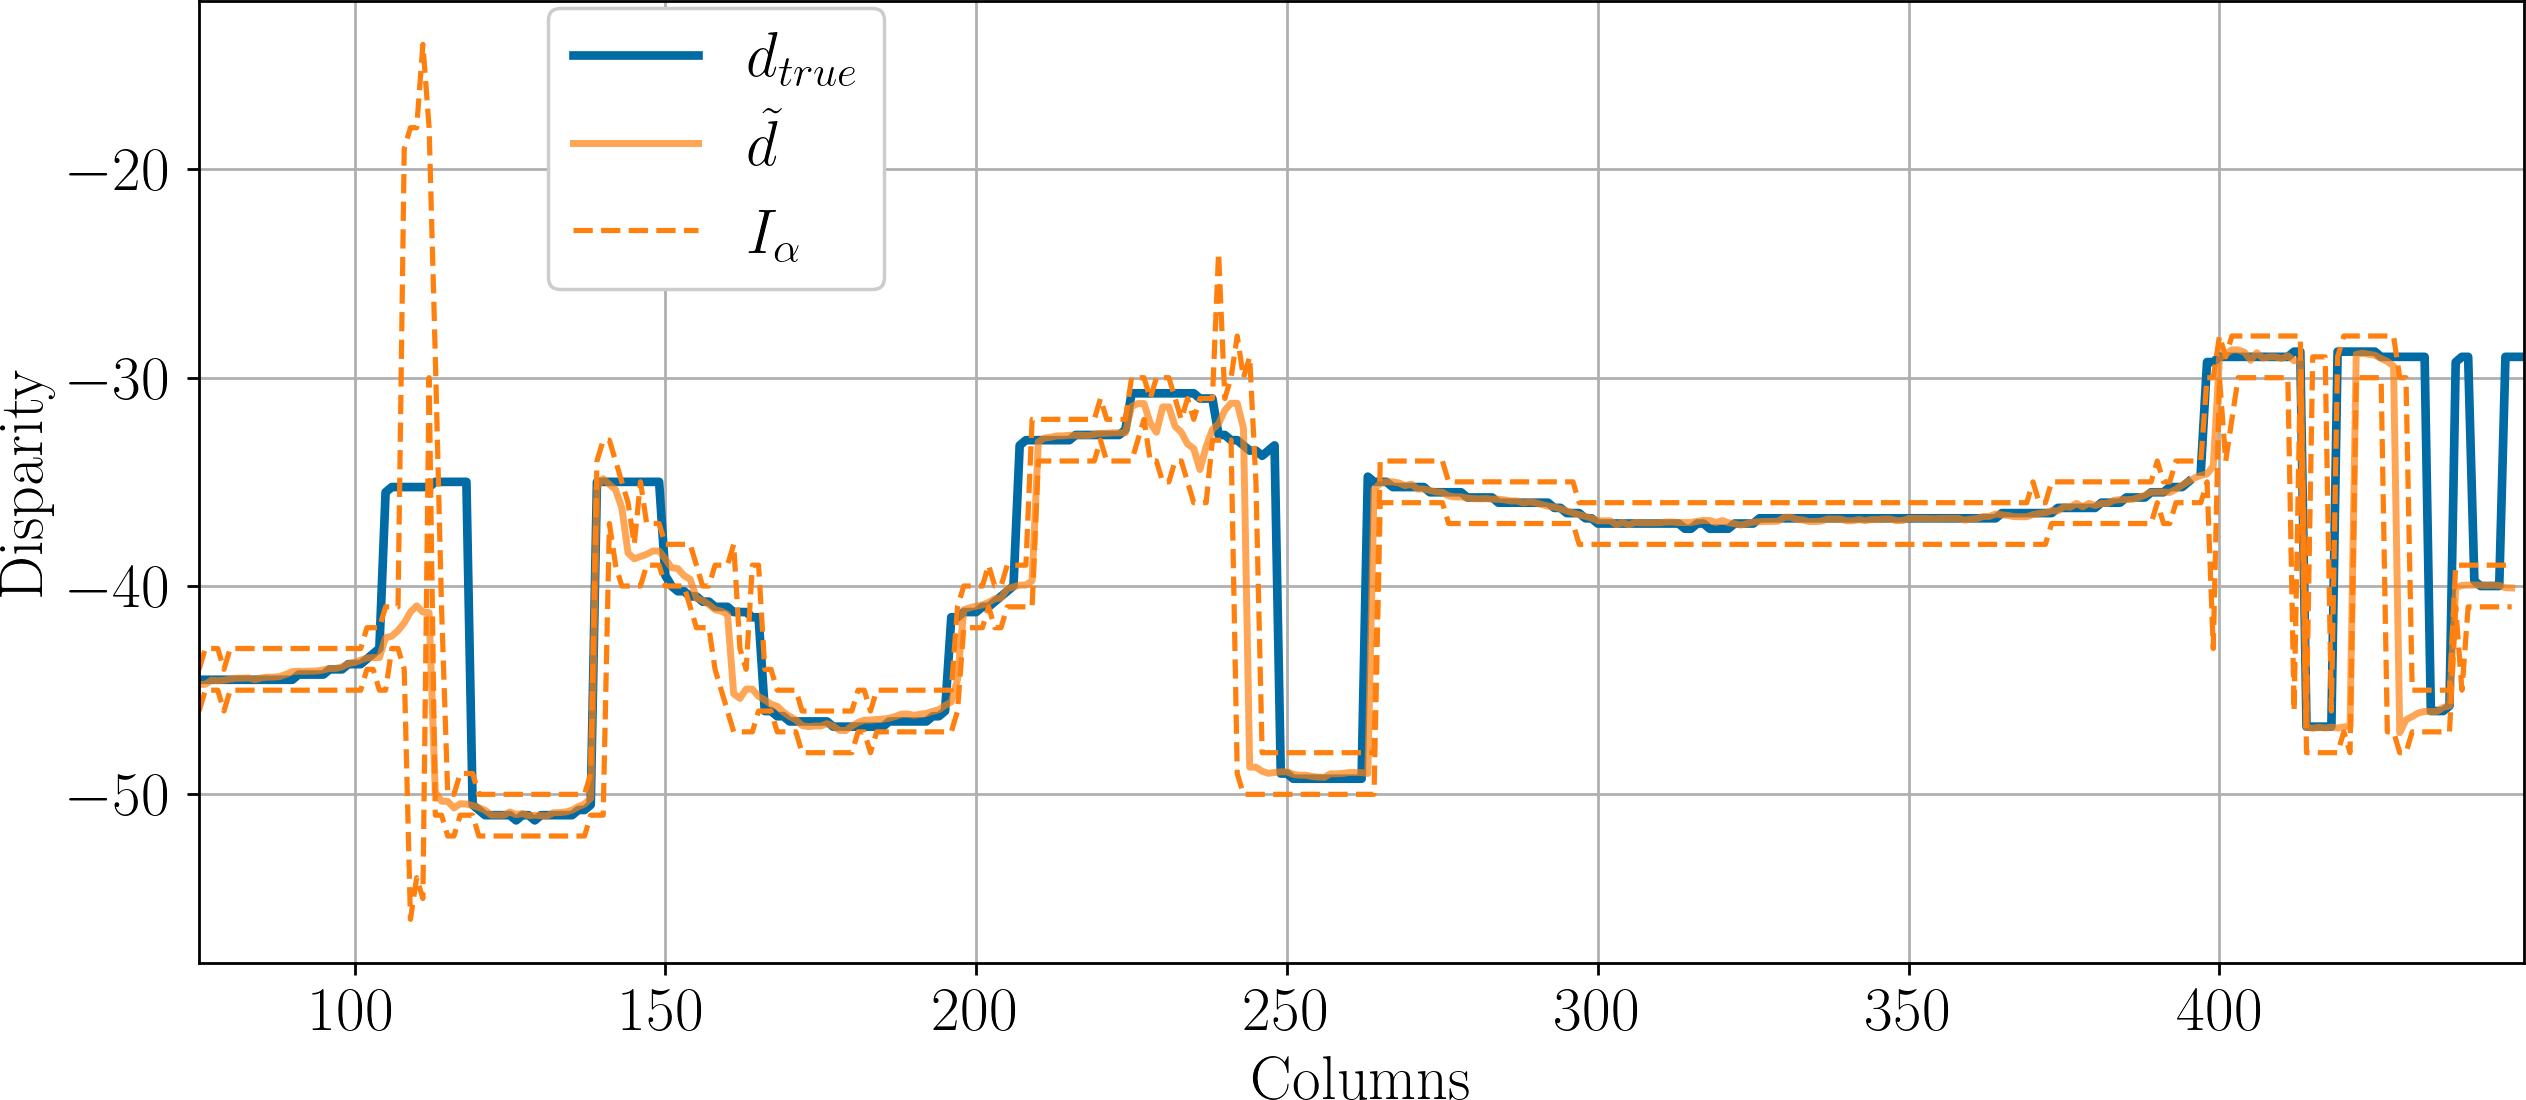
\includegraphics[width=\linewidth]{Images/Chap_5/intervals_ambiguous_area_row_240_1.png}
        \caption{$I_\alpha$ along row $240$}
        \label{fig:intervals_ambiguous_row_240_no_reg}
    \end{subfigure}\hfill
    \begin{subfigure}[t]{\linewidth}
        \centering
        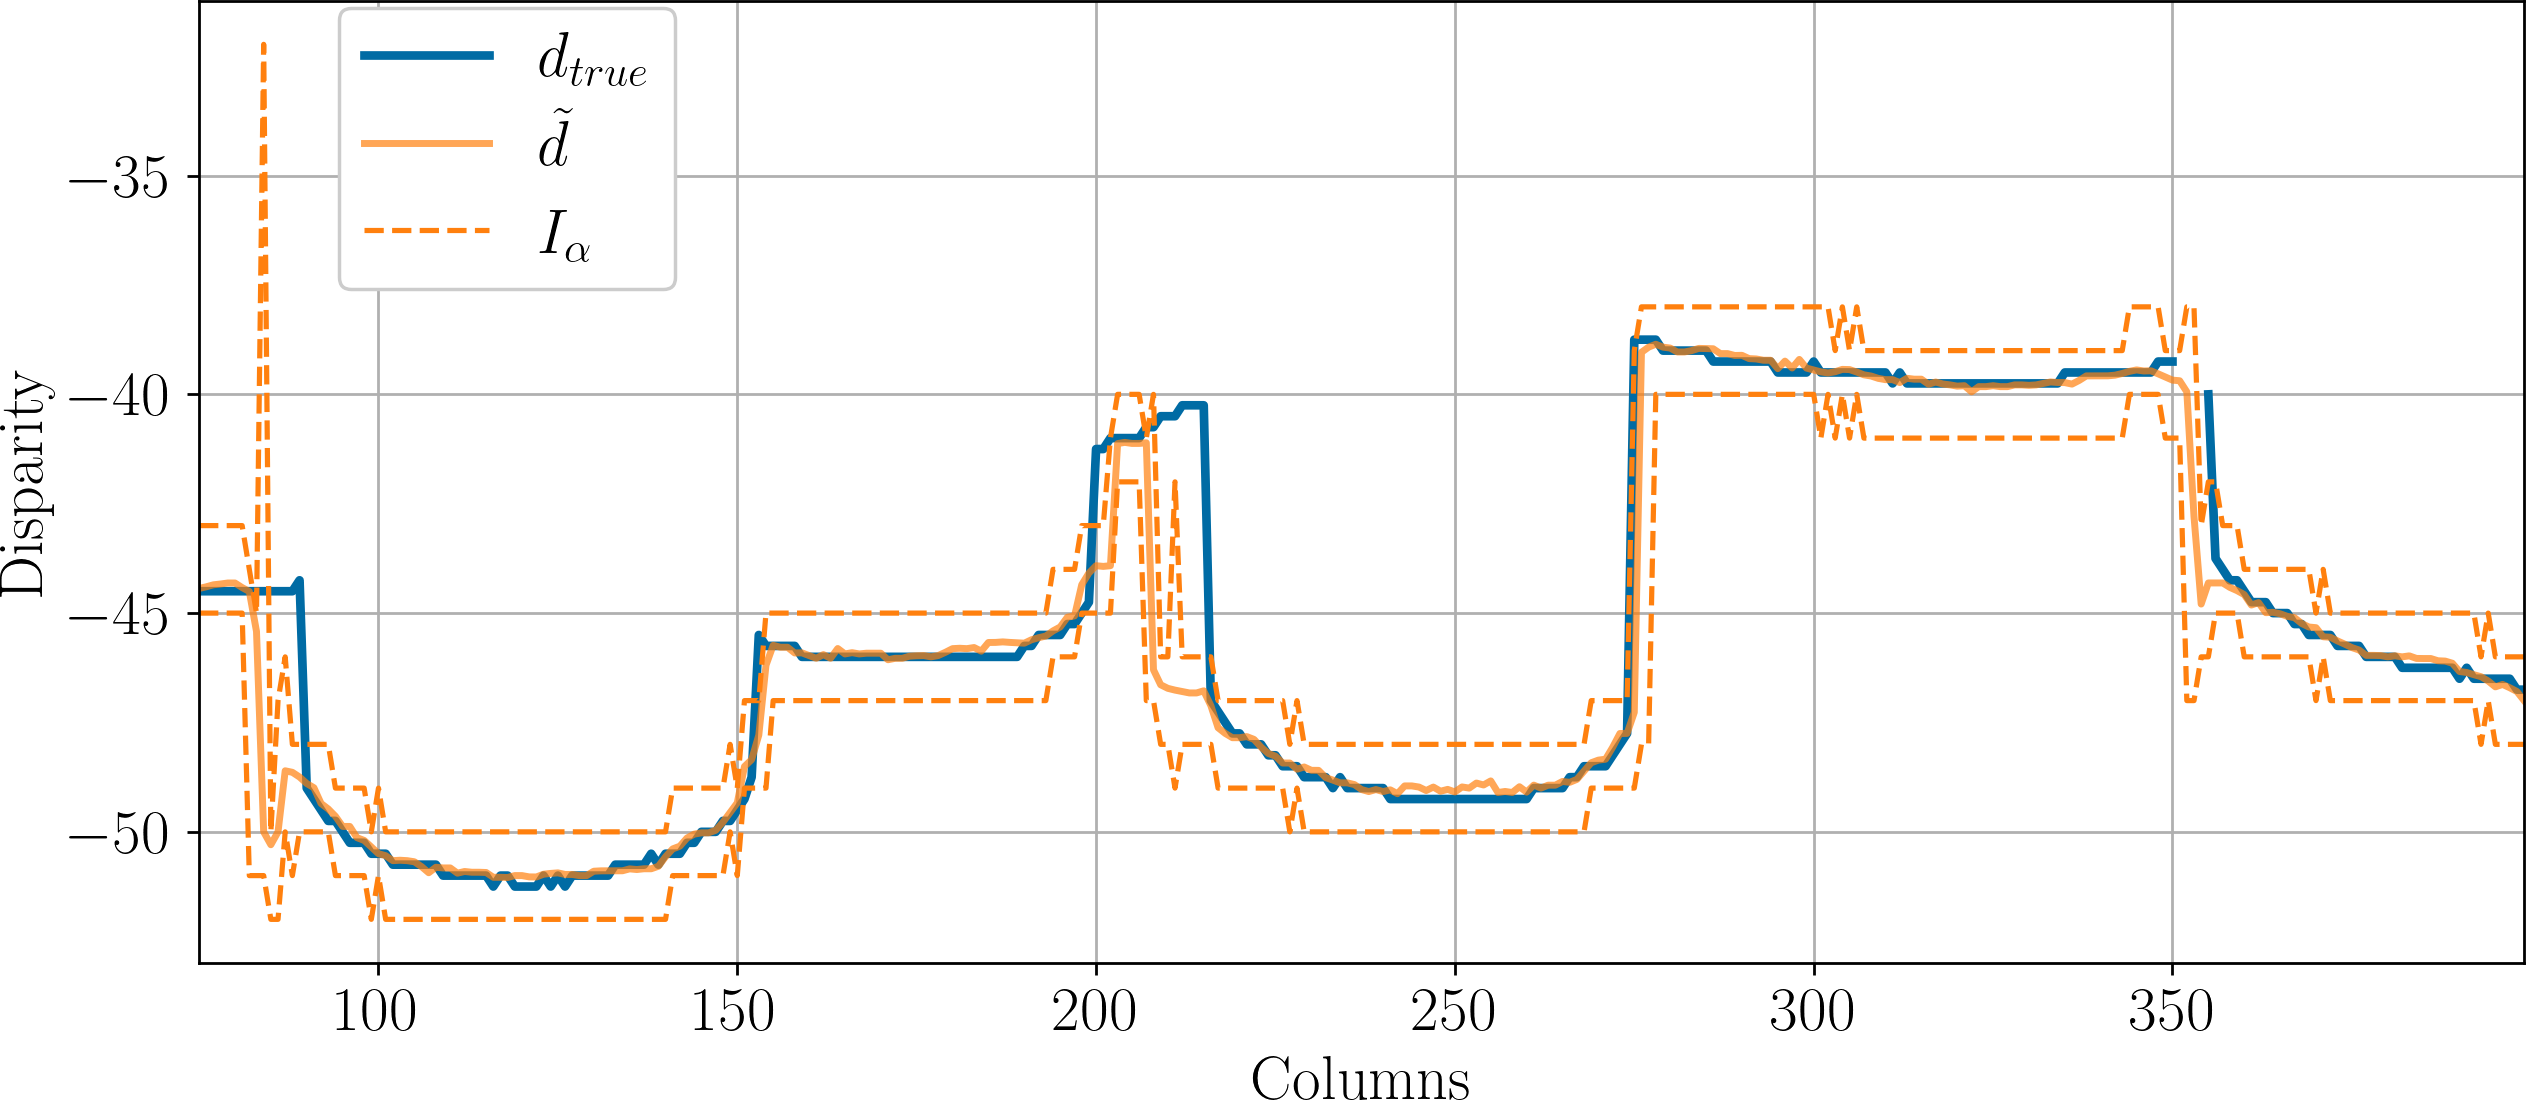
\includegraphics[width=\linewidth]{Images/Chap_5/intervals_ambiguous_area_row_290_1.png}
        \caption{$I_\alpha$ along row $290$}
        \label{fig:intervals_ambiguous_row_290_no_reg}
    \end{subfigure}
    \caption{$I_\alpha$ for the two bottom rows highlighted in \Cref{fig:cones_with_rows}.}
    \label{fig:intervals_ambiguous_row_240_290}
\end{figure}

By construction, $I_\alpha$ will always contain the predicted disparity $\tilde{d}$ as the maximum of each possibility curve will also be selected as the predicted disparity by winner-takes-all strategy. However, we are interested to see if intervals can contain the true disparity $d_{true}$ even when the predicted disparity is far from it. \Cref{fig:intervals_ambiguous_row_80_180,fig:intervals_ambiguous_row_240_290} represent the disparity intervals $I_\alpha$, predicted disparity $\tilde{d}$ and true disparity $d_{true}$ for the different rows. A first observation is that intervals correctly contain the true disparity in regions where there are no strong variations of disparities. In  \Cref{fig:intervals_ambiguous_row_180_no_reg}, intervals in columns $50$ to $75$ and around $175$ are much larger than in the rest of the figure. In those areas, the predicted disparity is also far from the ground truth. This translates the fact that the method for creating intervals is able to detect the difficulties encountered by the correlator when predicting a disparity, and to adapt the size of intervals consequently. On the downside, we can see that near strong variations of the disparity, intervals tend to ``miss'' the discontinuities. Indeed, they do not contain the true disparity around those areas, as observed near columns $215$ and $250$ of \Cref{fig:intervals_ambiguous_row_80_no_reg}, columns $95$, $125$ of \Cref{fig:intervals_ambiguous_row_180_no_reg}, columns $100$, $115$, $150$, $200$, $250$ of \Cref{fig:intervals_ambiguous_row_240_no_reg} 
and finally columns $90$, $200$ and $220$ of \Cref{fig:intervals_ambiguous_row_290_no_reg}.

The method presented in this section seems to offer a good estimation of the error in the disparity estimation step. Some errors remain near disparity discontinuities, which we will try to rectify in \Cref{sec:regularization_of_intervals}.

\subsection{Ensuring Coherence Between the Predicted Disparity and Confidence Intervals}\label{sec:coherence_disparity_intervals}
We propose a method for creating confidence intervals that should include the true disparity at least $90\%$ of the time. It should, however, always include the predicted disparity $\tilde{d}$. Indeed, it would not make much sense to provide a confidence interval and a prediction that is not included in the interval. As $\tilde{d}$ is the maximum of each possibility curve, it will also be selected as the predicted disparity by the winner-takes-all strategy and will thus belong to the confidence interval. However, the disparity map $\tilde{d}$ is often post-processed to improve its quality, mainly using a filtering and a refinement step. Those steps modify the disparity map, and we must ensure we modify the confidence intervals accordingly so that they remain coherent with the predicted disparity. 

As detailed in \Cref{sec:stereo_matching}, a filtering step is usually carried out on the disparity map in order to remove potential outliers. The filter applied in our experiments and in many other pipelines is a median filter \cite{scharstein_taxonomy_2001}. Applying the filter only to the disparity map without processing the intervals accordingly can result in inconsistencies, as illustrated in \Cref{fig:median_filtering}. Fortunately, separately applying the same median filter to the lower bounds and upper bounds of the intervals is sufficient to ensure coherence. Indeed, because for all pixels $p_1\enum p_n$ considered in the filtering, it holds:
\begin{align}
    \underline{I}_\alpha(p_i)\leqslant \tilde{d}(p_i) \leqslant \overline{I}_\alpha(p_i)
\end{align}
then it is possible to prove that
\begin{align}
    \median_{p_1\enum p_n} \underline{I}_\alpha(p_i)\leqslant \median_{p_1\enum p_n}\tilde{d}(p_i) \leqslant \median_{p_1\enum p_n}\overline{I}_\alpha(p_i)
\end{align}
The proof of this result can be found in the \hyperref[chap:annex]{Annex}, using \Cref{prop:median_consistency}.

\begin{figure}
    \centering
    \begin{subfigure}[t]{0.32\linewidth}
        \centering
        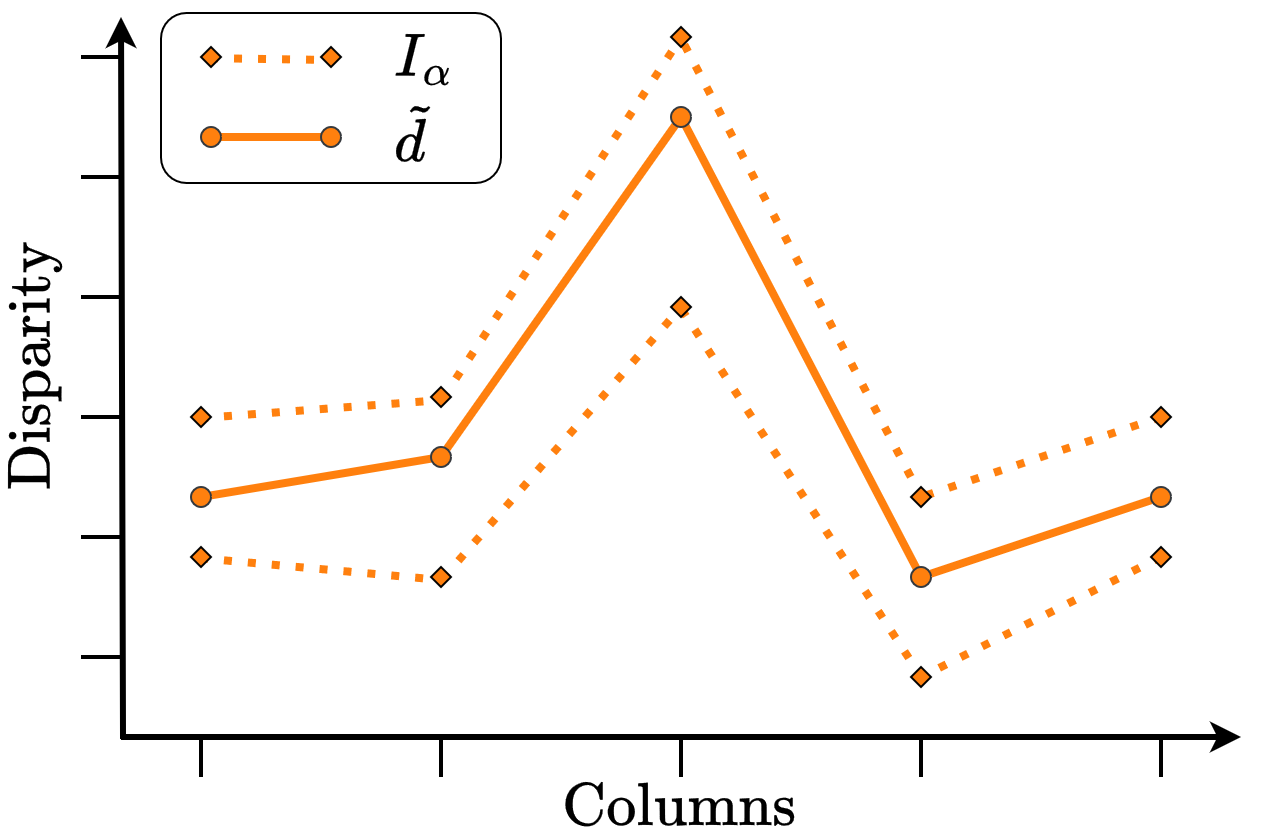
\includegraphics[width=\linewidth]{Images/Chap_5/Median_filtering_1.png}
        \caption{Without filtering}
        \label{fig:median_filtering_1}
    \end{subfigure}
    \hfill\begin{subfigure}[t]{0.32\linewidth}
        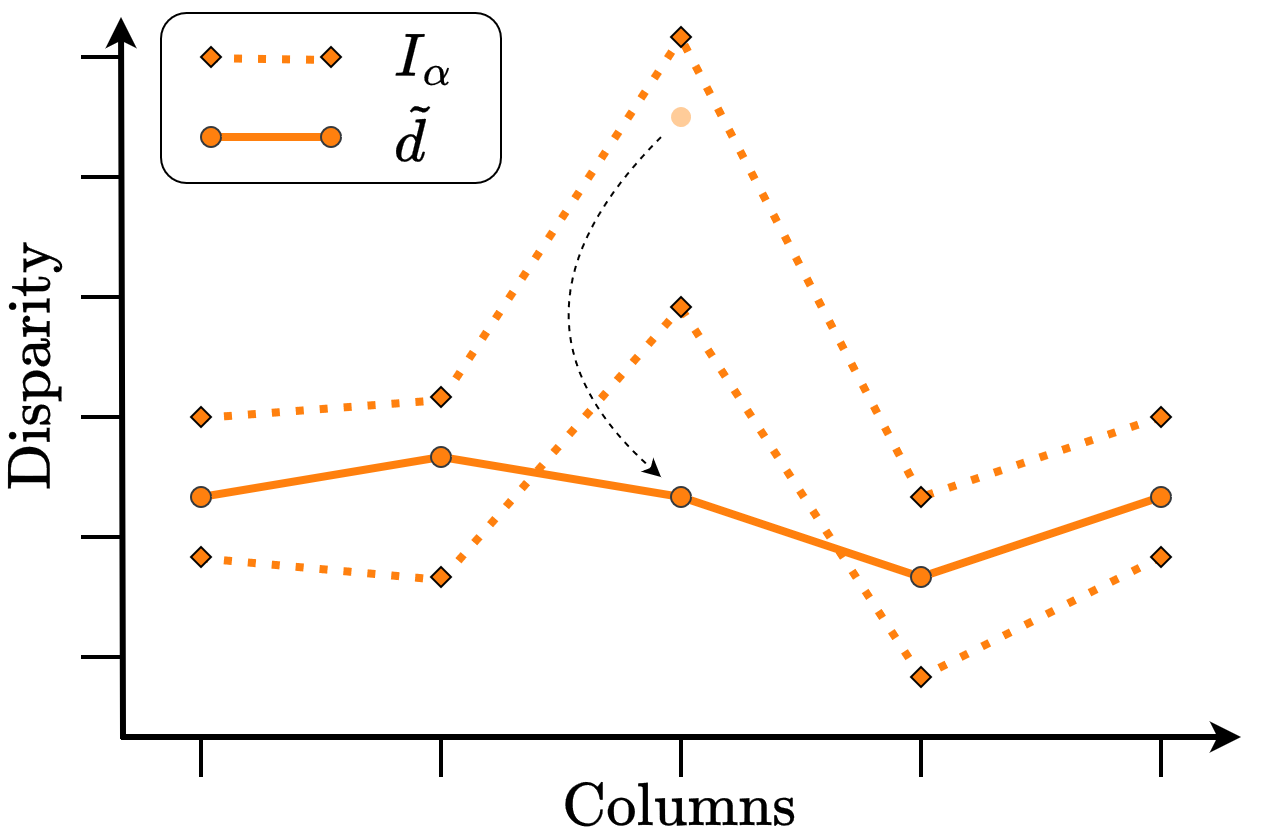
\includegraphics[width=1\linewidth]{Images/Chap_5/Median_filtering_2.png}
        \caption{Filtering only $\tilde{d}$}
        \label{fig:median_filtering_2}
    \end{subfigure}\hfill
    \begin{subfigure}[t]{0.32\linewidth}
        \centering
        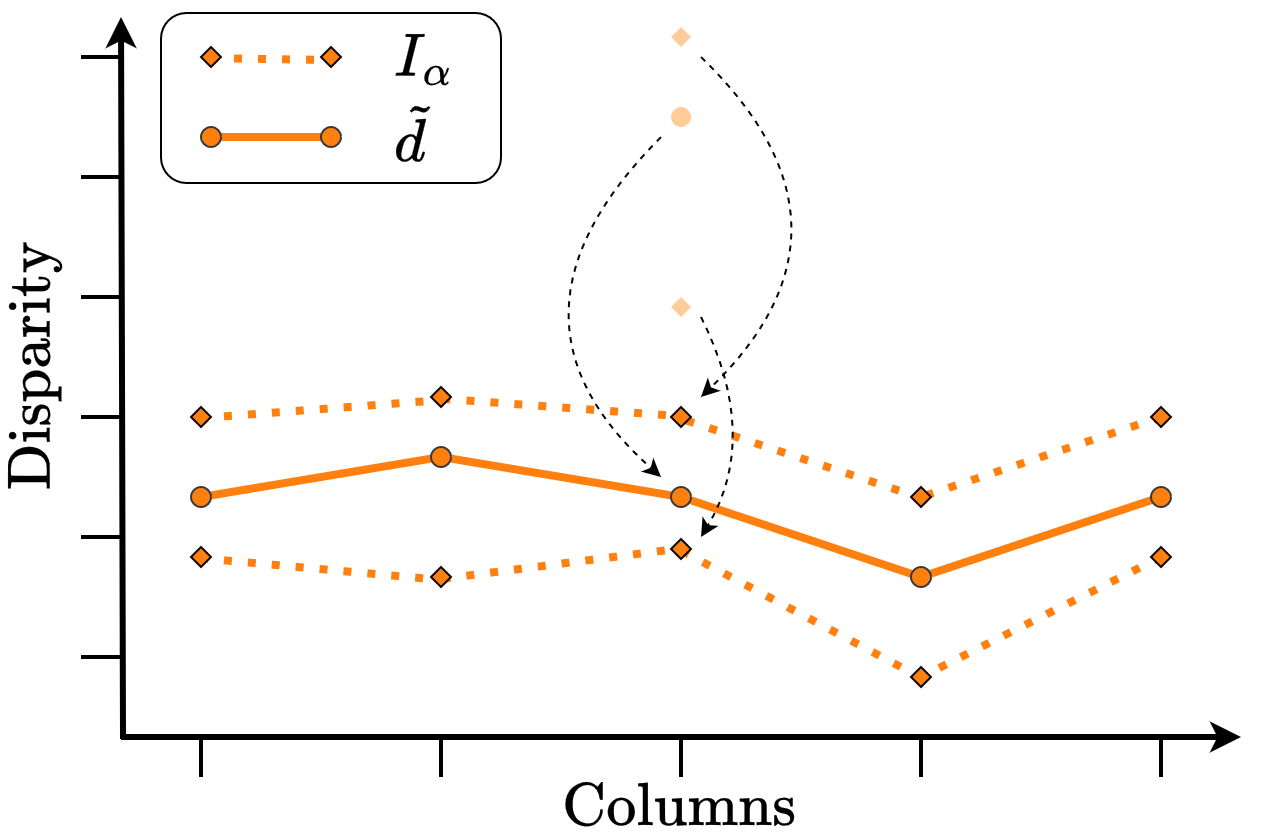
\includegraphics[width=\linewidth]{Images/Chap_5/Median_filtering_3.png}
        \caption{Filtering $\tilde{d}$ and $I_\alpha$}
        \label{fig:median_filtering_3}
    \end{subfigure}
    \caption{Effect of a median filter on the predicted disparity $\tilde{d}$ and confidence intervals $I_\alpha$. For the sake of the example, we only filter the middle point by looking at its neighbors. \subref{fig:median_filtering_1} contains the unfiltered curves. \subref{fig:median_filtering_2} contains unfiltered intervals, and filtered $\tilde{d}$. \subref{fig:median_filtering_3} filtered intervals and filtered $\tilde{d}$.}
    \label{fig:median_filtering}
\end{figure}

Another processing applied to the disparity map is the sub-pixel refinement of its values, presented in \Cref{sec:stereo_matching} and \Cref{fig:sub-pixel_refinement}. The idea is to slightly modify the value of the disparity by interpolation of the cost curve, in order to obtain sub-integers disparity values. The modification cannot change a disparity more than a pixel away from its original value. If the predicted disparity $\tilde{d}$ equals one of the bounds of its confidence interval $I_\alpha$, the sub-pixel refinement step can shift the predicted disparity to a value slightly outside the confidence intervals. In this case, we simply extend the interval by one pixel. For instance, if $\tilde{d}=\underline{I}_\alpha$, then the new confidence interval $I_\alpha'$ equals:
\begin{align}\label{eq:subpixel_intervals}
    I_\alpha'=[\underline{I}_\alpha-1,~\overline{I}_\alpha]
\end{align}
This stretching is simple, and also presents the advantage of working with any type of sub-pixel refinement that do not modify the predicted disparity value from more than $1$ pixel (\ie V-fit, parabola \etc).

\subsection{Regularization of Intervals in Low Confidence Areas}\label{sec:regularization_of_intervals}
Disparity intervals estimation has the potential to perform well even when the predicted disparity is far away from the ground truth. This model however encounters some performance issues near depth discontinuities, and does not currently satisfy the aimed $90\%$ accuracy objective (see \hyperref[chap:annex]{Annex}). This can be explained as follows: as the \acrshort{sgm} regularization attempts to impose continuity on disparities, it results in cost curves that do not favor the correct disparity in the region where the continuity hypothesis is not valid. Considering that cost curves are equivalent to experts' opinions in those areas can be over-optimistic, and the resulting intervals thus cannot be completely trusted. We will now present how we can adapt the model in those regions, in order to correct those flaws.

The first challenge to tackle is to determine if we are able to detect regions where discontinuities occur, in order to process intervals differently in those regions. Using the predicted disparity map might be a lead, but we saw in \Cref{fig:intervals_ambiguous_row_80,fig:intervals_ambiguous_row_180,fig:intervals_ambiguous_row_240,fig:intervals_ambiguous_row_290} that there is usually a shift between predicted disparity discontinuities and true disparity discontinuities. Instead, we could consider to use confidence measures computed alongside the disparity map, which are usually good candidates to detect discontinuities. In particular, we chose the confidence from ambiguity measure $c_{amb}$ presented in \Cref{eq:confidence_from_ambiguity} from \Cref{chap:stereophotogrammetry}. As a reminder, the confidence from ambiguity of a cost curve is computed as follows: given a value $\eta>0$, we compute the number of disparities whose cost is within $\eta$ to the minimum of the cost curve, then we compute the integral for all $\eta$ and normalize it between $0$ and $1$. It is formally transcribed by the following equations from \Cref{sec:uncertainty_pandora}:
\begin{align*}
    &amb(\rowcol, ~\eta) = \#\{d ~|~ C_V(row,~col,~d) \leqslant \min_\delta C_V(\rowcol, ~\delta) + \eta\}\\
    &\mathrm{AUC}_{amb}(\rowcol) = \frac{1}{\max\eta-\min\eta}\int_\eta amb(row,~col,~\eta)d\eta\\
    &c_{amb}(\rowcol) = \frac{\max \mathrm{AUC}_{amb}- \mathrm{AUC}_{amb}(\rowcol)}{\max \mathrm{AUC}_{amb} -\min \mathrm{AUC}_{amb}}
\end{align*}

Note that other confidence measures could be considered instead of the ambiguity, but this confidence measure has the advantage of performing well, being explainable (which is not always the case for confidence measures based on deep learning) and being already implemented in the stereo pipeline we use. \Cref{fig:wrong_intervals_and_ambiguity} shows that pixels with wrong intervals $I_\alpha$ usually present a low confidence from ambiguity as well, meaning that we can use this confidence measure to process confidence intervals differently.

\begin{figure}
    \centering
    \begin{subfigure}[t]{0.3\linewidth}
        \centering
        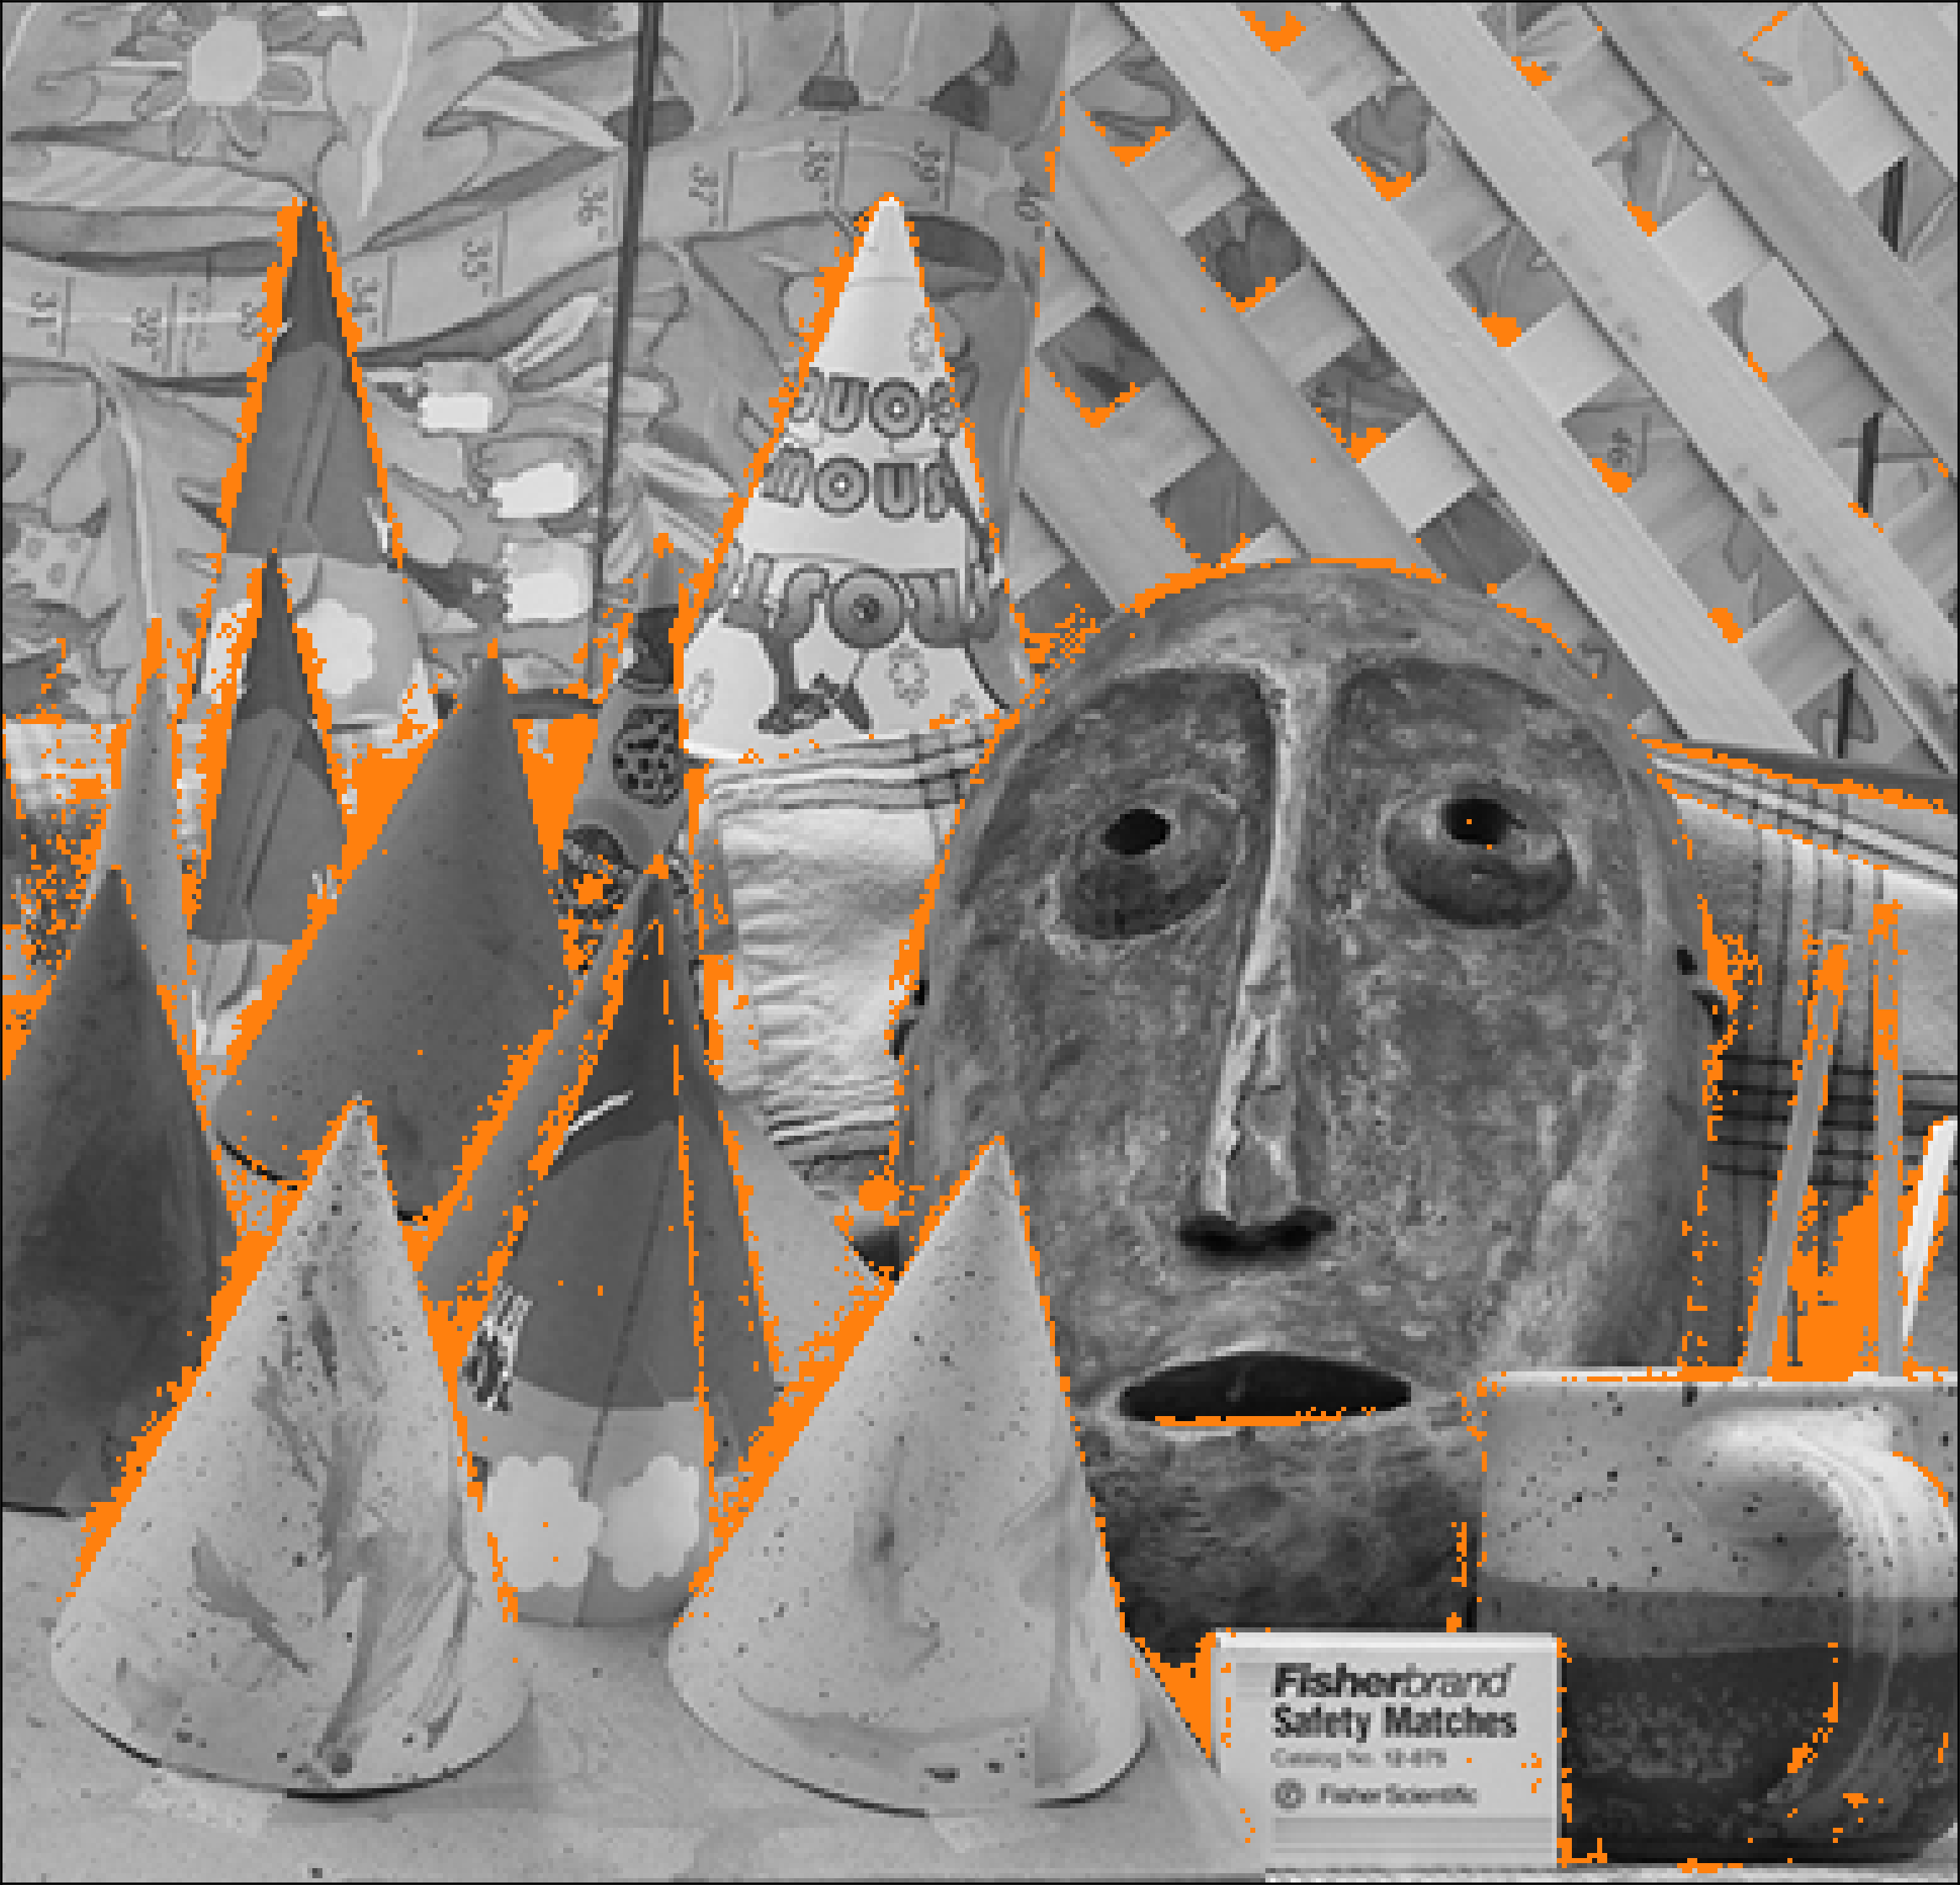
\includegraphics[width=\linewidth]{Images/Chap_5/wrong_intervals_no_reg.png}
        \caption{Left stereo image. Pixels where $d_{true}\not\in I_\alpha$ appear in orange.}
        \label{fig:wrong_intervals}
    \end{subfigure}\hfill
    \begin{subfigure}[t]{0.3\linewidth}
        \centering
        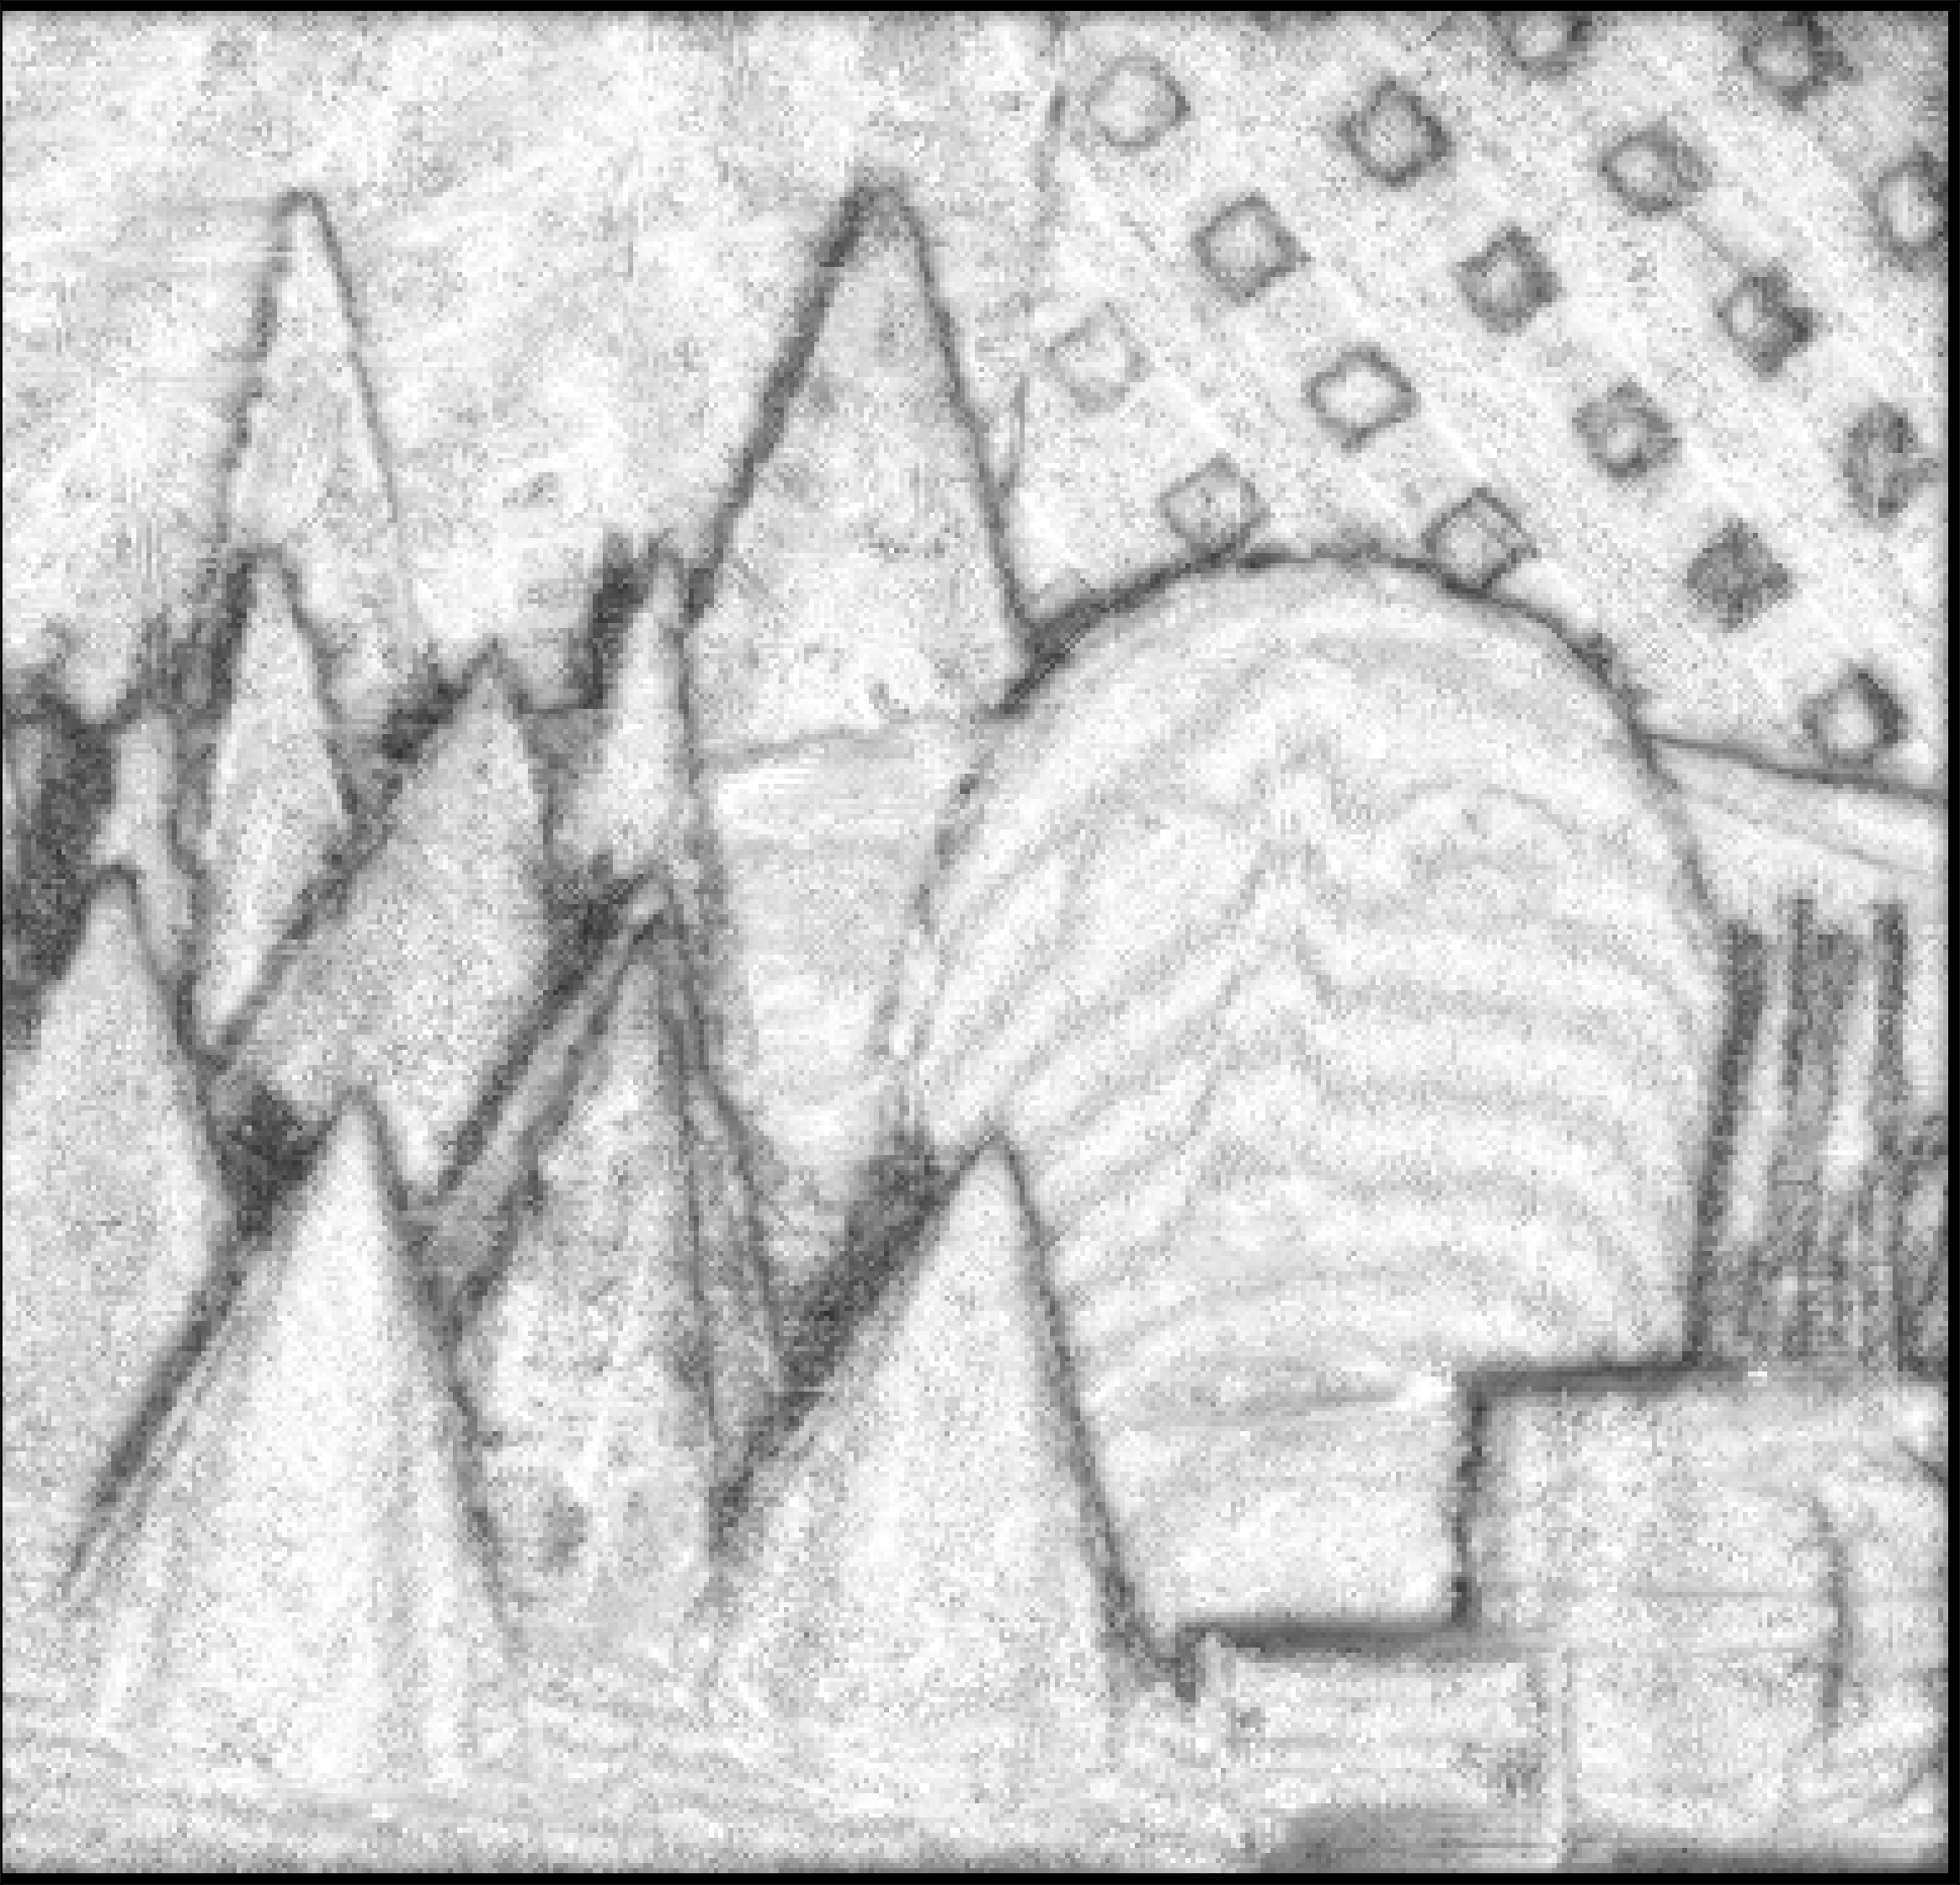
\includegraphics[width=\linewidth]{Images/Chap_5/ambiguity_cones.png}
        \caption{Confidence from ambiguity $c_{amb}$. Dark pixels have a low confidence, bright pixels have a high confidence.}
        \label{fig:ambiguity_cones}
    \end{subfigure}\hfill
    \begin{subfigure}[t]{0.3\linewidth}
        \centering
        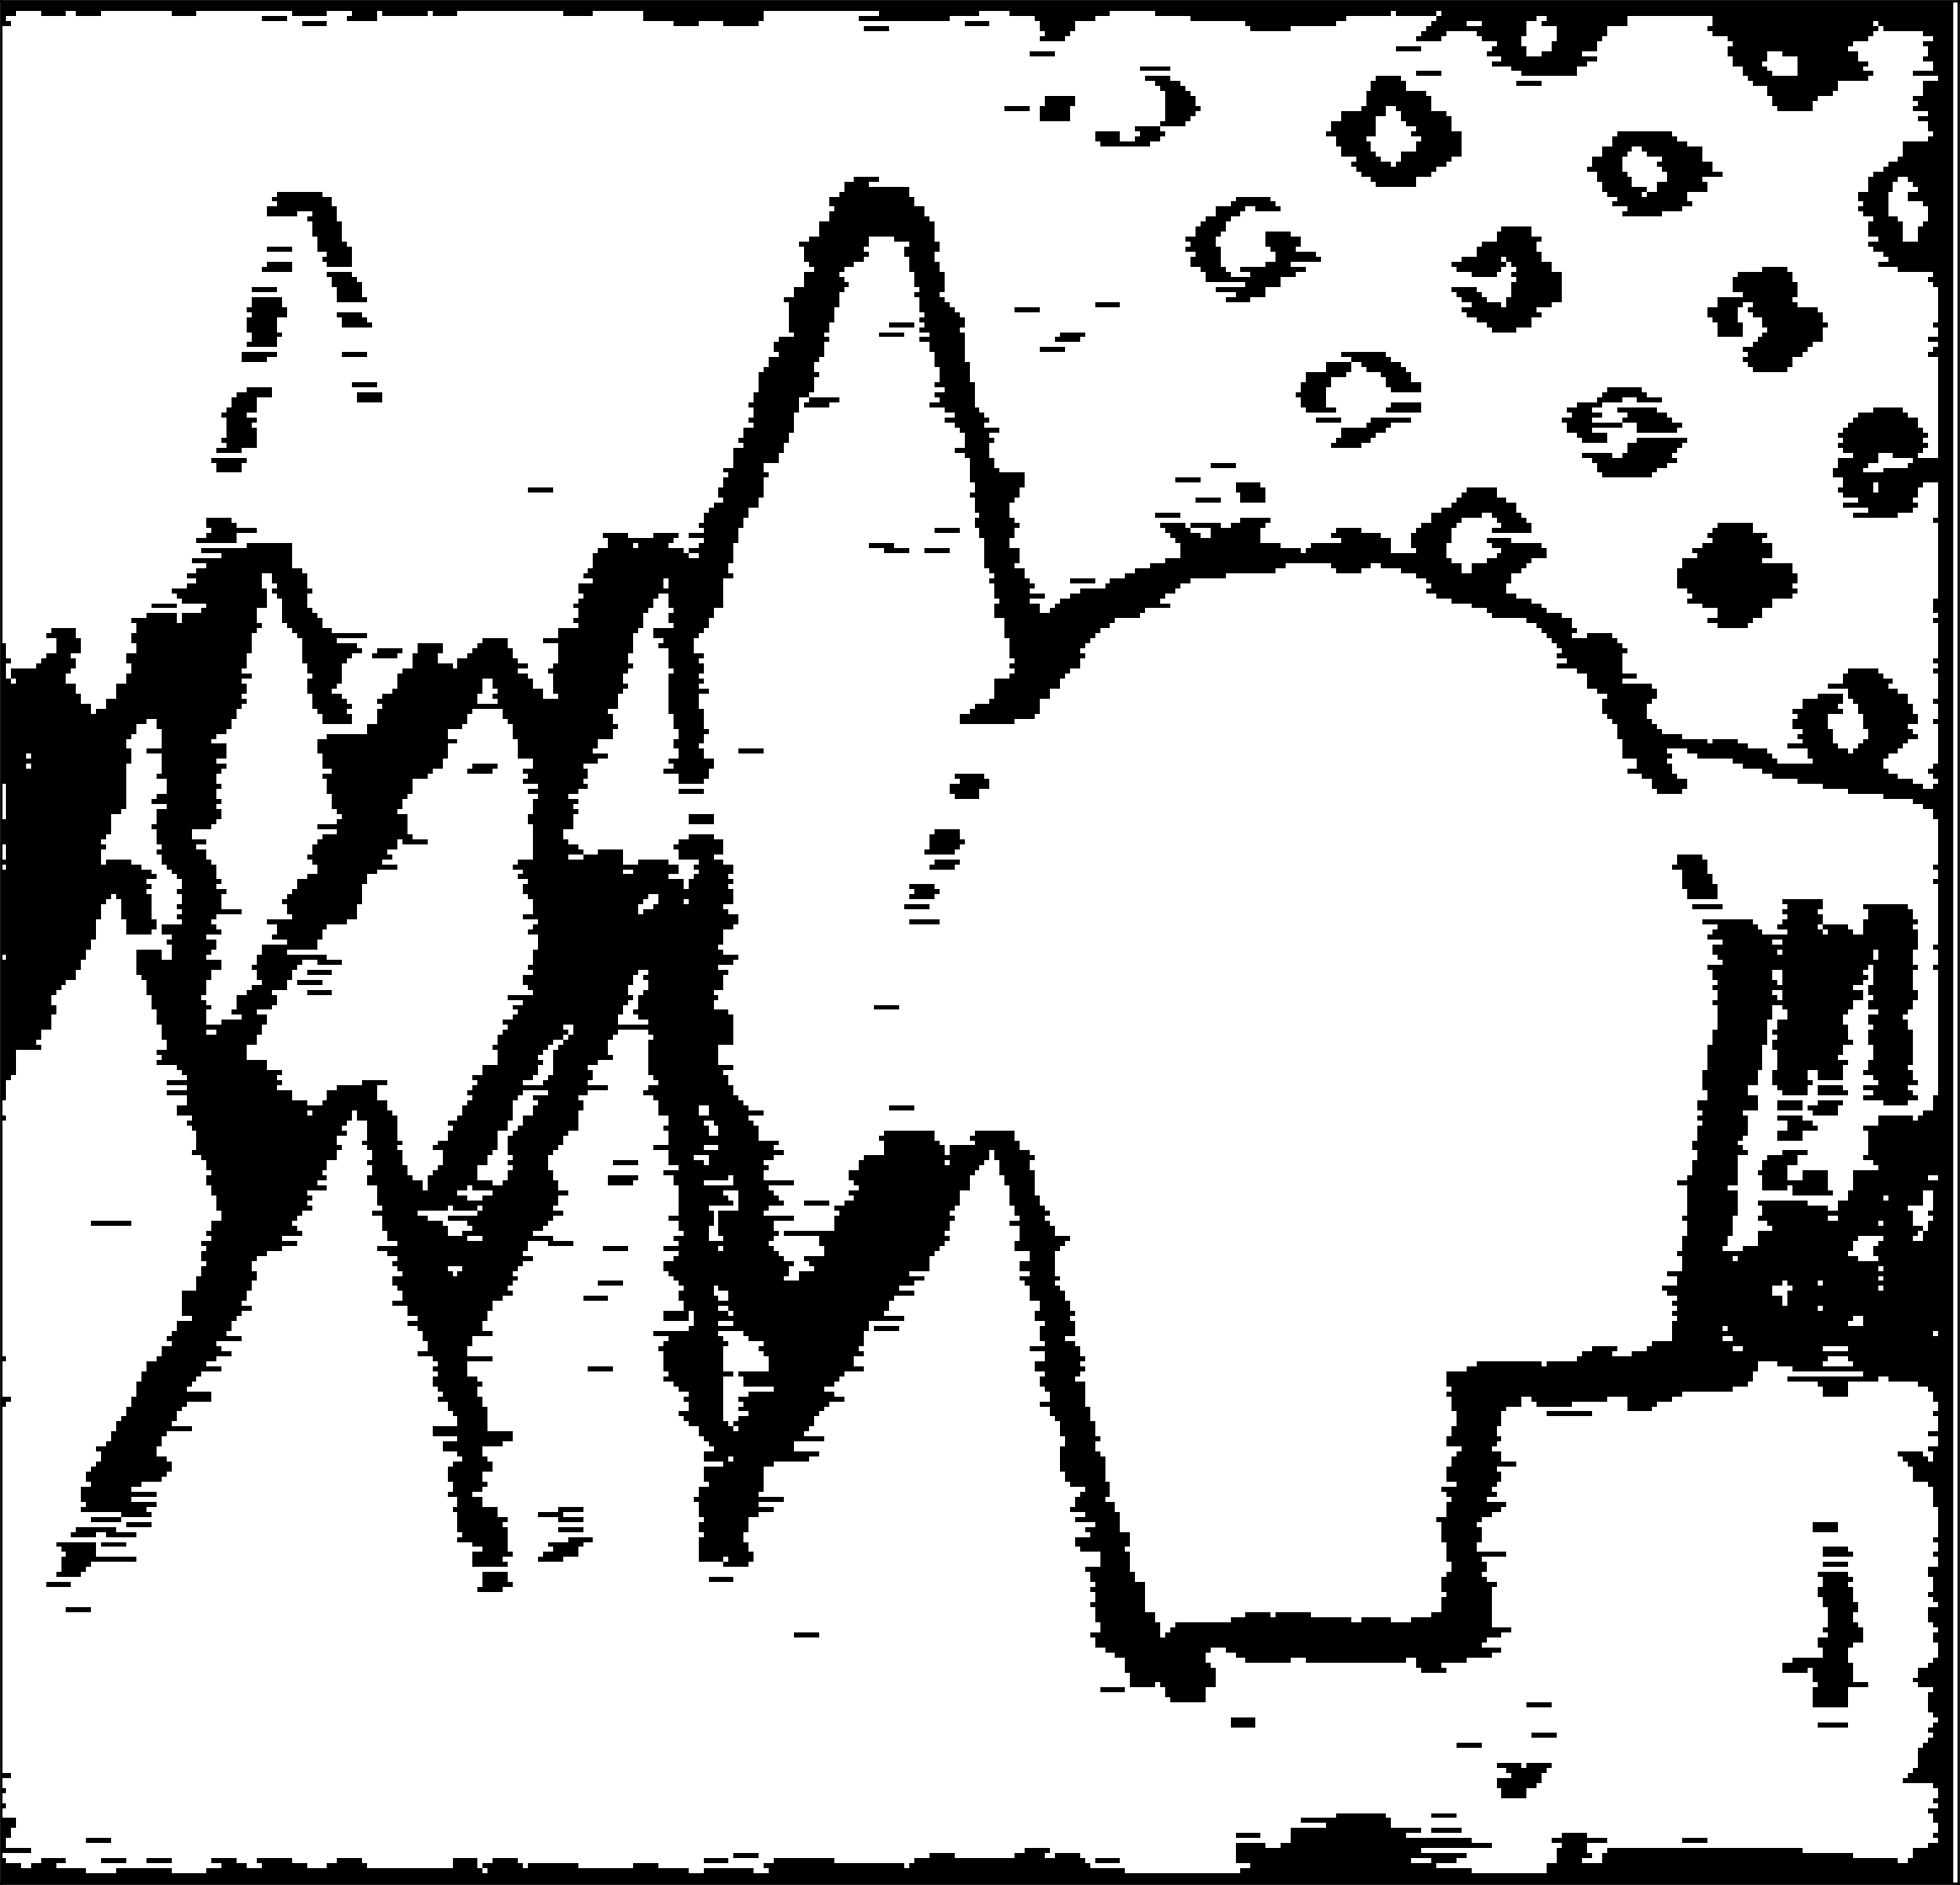
\includegraphics[width=\linewidth]{Images/Chap_5/ambiguity_mask_cones.png}
        \caption{Binary mask, low confidence areas are indicated by black pixels.}
        \label{fig:ambiguity_mask_cones}
    \end{subfigure}
    \caption{Position of wrong intervals in the left image, the corresponding confidence map and the low confidence area mask obtained using \Cref{eq:low_confidence_area}}
    \label{fig:wrong_intervals_and_ambiguity}
\end{figure}

The method developed for detecting low confidence areas is to apply a simple threshold $\tau_{amb}$ on the confidence from ambiguity $c_{amb}$. However, $c_{amb}$ is computed pixel-wise, which can lead to high-frequency spatial variations of the confidence. To smooth the ambiguity curve, a minitive kernel of size $(1, ~2\times k_{amb}+1)$ is applied. A pixel $(\rowcol)$ is thus considered to be in a low confidence area if it verifies:
\begin{align}\label{eq:low_confidence_area}
    \min_{-k_{amb}~\leqslant~ k~\leqslant ~k_{amb}}c_{amb}(\rowcol+k)\leqslant \tau_{amb}
\end{align}
We used $k_{amb}=2$ and $\tau_{amb}=0.6$ in our experiments. For simplicity, we will refer to $\min c_{amb}$ instead of $min_{-k_{amb}~\leqslant~ k~\leqslant ~k_{amb}}c_{amb}$ in the following. Additional investigations on those parameters are presented in the \hyperref[chap:annex]{Annex}. \Cref{fig:ambiguity_kernel} illustrates the impact of smoothing the confidence from ambiguity, and displays the threshold used to detect low confidence areas. We can see around columns $185$ and $320$ that the kernel smooths isolated confidence values that would not be detected by the threshold otherwise. \Cref{fig:ambiguity_mask_cones} presents the position of pixels in low confidence areas over the whole left image. As a quick indicator of this method performance, $83\%$ of intervals that do not contain the ground truth (orange pixels in \Cref{fig:wrong_intervals}) are also contained in low confidence areas. Once again, it is possible to use any other confidence measure to detect areas where intervals perform badly. The choice of this method in particular is motivated by its good performance while remaining simple in comprehension and implementation.

\begin{figure}
    \centering
    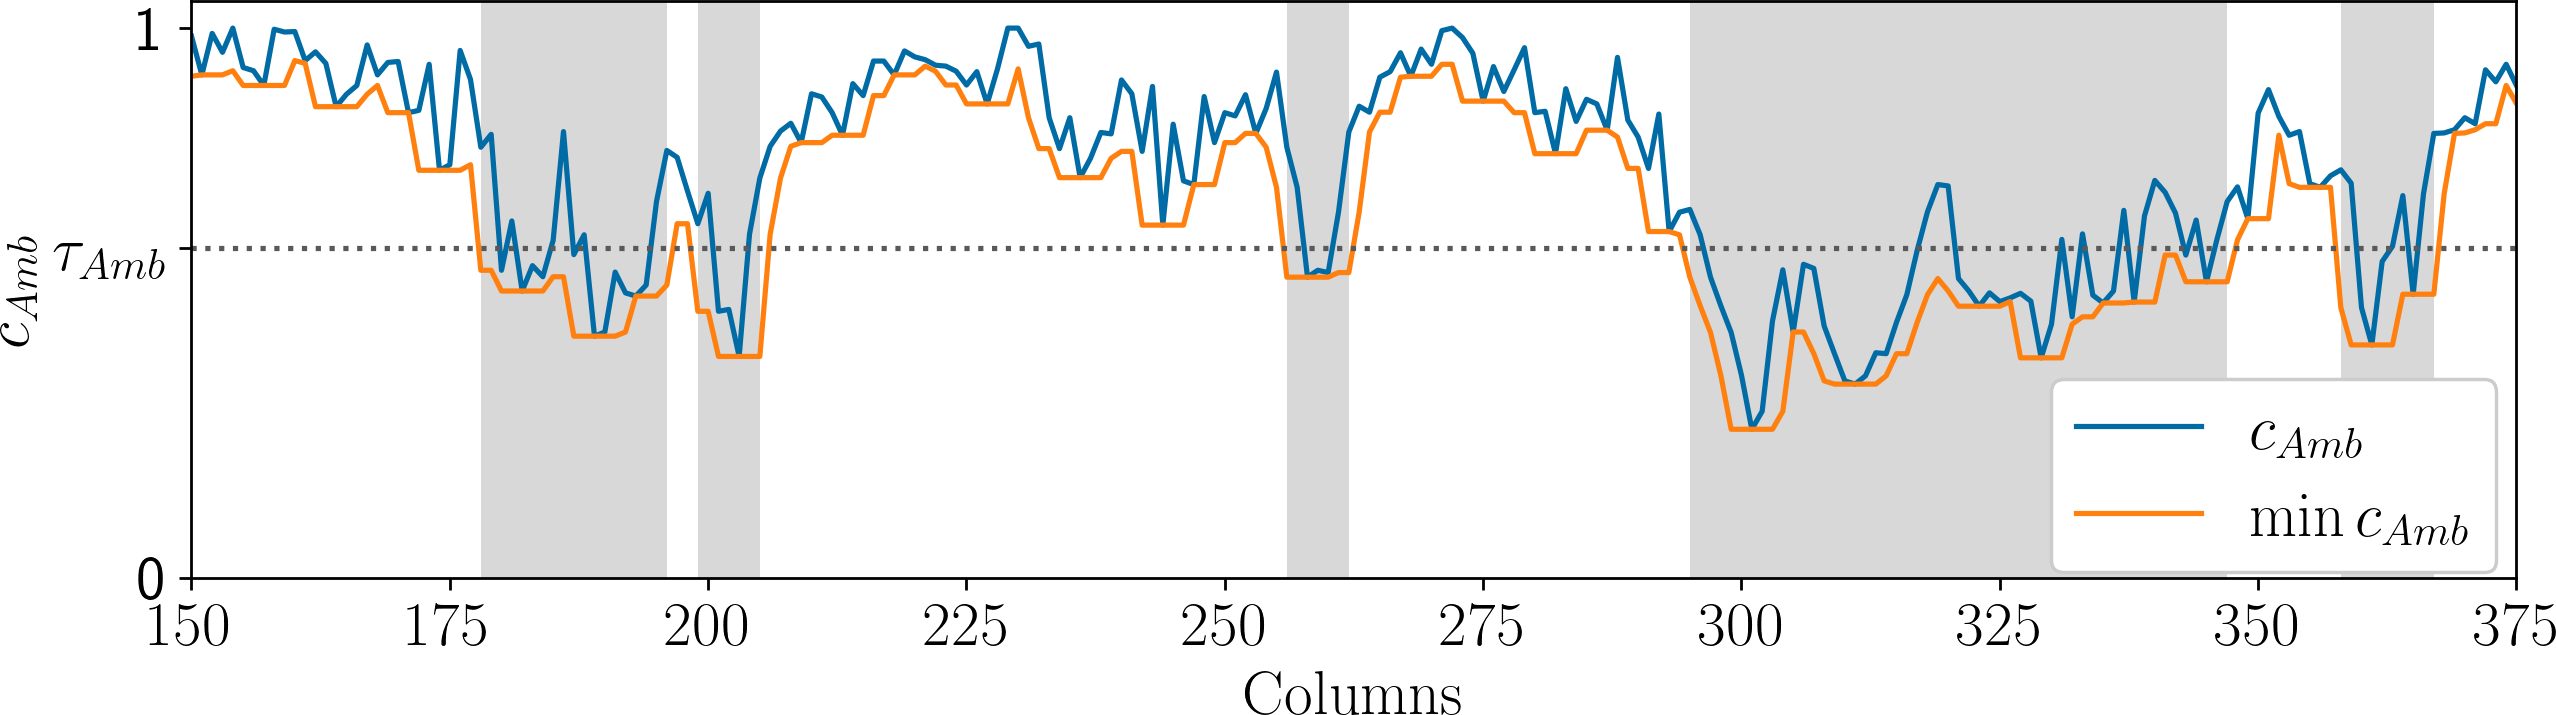
\includegraphics[width=\linewidth]{Images/Chap_5/ambiguity_kernel_row_110.png}
    \caption{Confidence from ambiguity $c_{amb}$ and smoothed confidence $\min c_{amb}$ from \Cref{eq:low_confidence_area} for row $110$ of the Middlebury Cones image. Low confidence areas, where $\min c_{amb}$ is less than $\tau_{amb}$ are highlighted in gray.}
    \label{fig:ambiguity_kernel}
\end{figure}

Having computed regions of low confidence, we can now process the intervals differently in those areas. The main idea here is that information contained in low confidence cost curves should be handled with care. The hypothesis that a cost curve can be interpreted as an expert stating his opinion on which disparities are most probable is questionable in those areas. We also cannot infer the confidence intervals from intervals in neighboring high confidence areas, as there is no guarantee the disparities are the same as their high confident neighbors. We instead chose to proceed in two steps. First, we compute a neighboring set of intervals for each low confidence pixel. Then, we use the information from this set to determine a new disparity interval by consensus. We modify the value of the considered pixel from this consensual interval.

We first detail how the set of neighboring pixels is determined. Let $(\rowcol)$ be a low confidence pixel. We define a segment $S(\rowcol)$ as the set containing $(\rowcol)$ and all adjacent low confidence pixels from the same row. An example of $S(\rowcol)$ is presented in \Cref{fig:low_confidence_segments} as an orange rectangle. Two segments $S(\rowcol)$ and $S(row+1, ~col')$ are considered adjacent if two of their pixels are directly on top of one another. The low confidence neighboring $\N(row,~col)$ is defined as the set of low confidence pixels in segment $S(\rowcol)$ or in adjacent segments within $n_\N$ rows. In practice, we use $n_\N=2$. $S(\rowcol)$ is formally defined as:
\begin{align}
    S(\rowcol) = \{~ (row,~col') \text{ \st }~\forall c\in\opi col, col'\cli,~\min c_{amb}(row, ~c+k)\leqslant \tau_{amb}~\}
\end{align}
where $\opi col,~col'\cli$ assumes that $col\leqslant col'$, and is replaced by $\opi col',~col\cli$ if not. The formal definition of the set of pixels $\N(row,~col)$ is then:
\begin{align}
    \N(row,~col) = \{ p\in &\bigcup_{-n_\N\leqslant k\leqslant n_\N}S(row+k, ~col_k)\nonumber\\
    &\st~S(row + (k+1), ~col_{k+1})\text{ is adjacent to }S(row+k, ~col_{k})\}\label{eq:n_N}
\end{align}
with $col_0=col$, and $n_\N$ the number of consecutive rows considered. \Cref{fig:low_confidence_segments} displays a graphical example of $S(\rowcol)$ and $\N(\rowcol)$ from the Middlebury Cones left image.

\begin{figure}
    \begin{subfigure}[t]{0.5\linewidth}
        \flushleft
        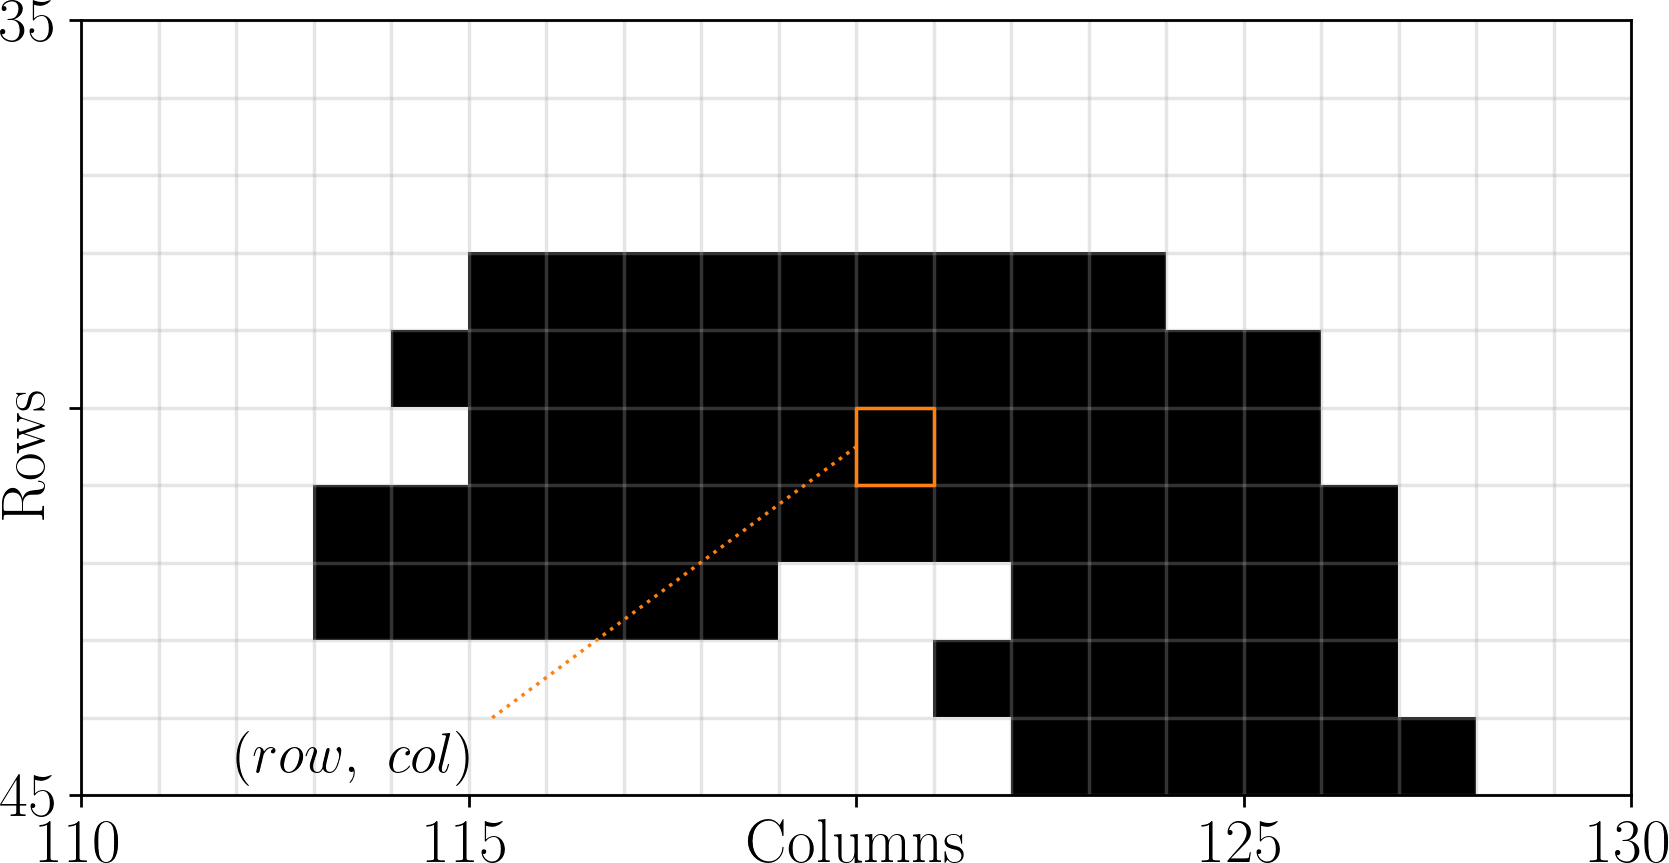
\includegraphics[width=\linewidth]{Images/Chap_5/low_confidence_segments_1.png}
        \caption{Low confidence pixel $(\rowcol)$}
        \label{fig:low_confidence_segments_1}
    \end{subfigure}
    \begin{subfigure}[t]{0.5\linewidth}
        \flushright
        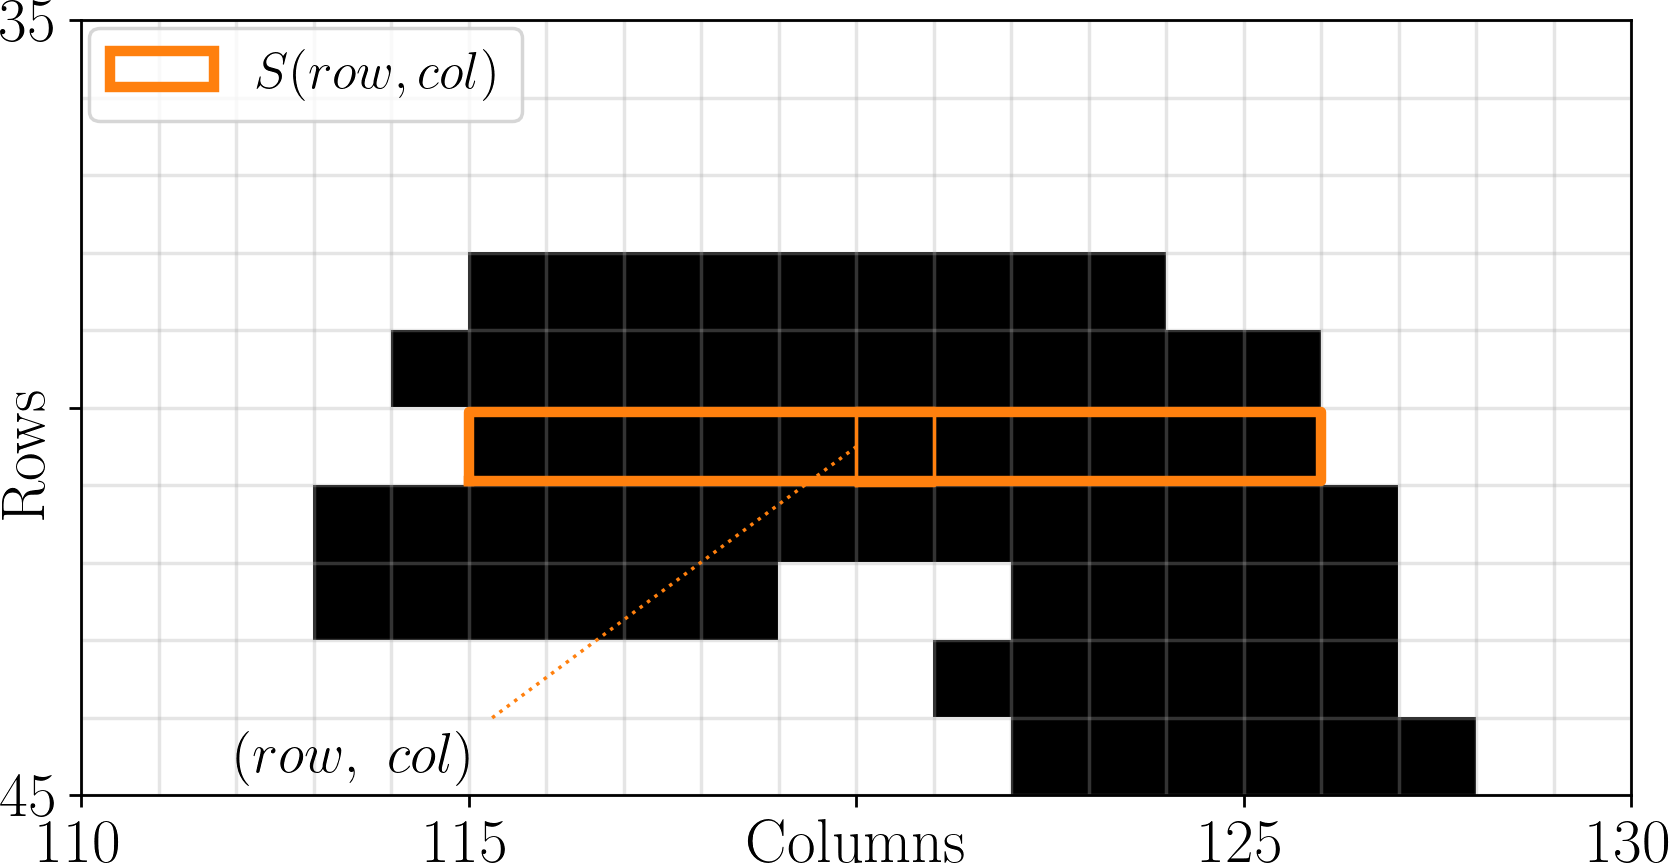
\includegraphics[width=\linewidth]{Images/Chap_5/low_confidence_segments_2.png}
        \caption{Segment $S(\rowcol)$}
        \label{fig:low_confidence_segments_2}
    \end{subfigure}\vspace*{0.3cm}
    \begin{subfigure}[t]{0.5\linewidth}
        \flushleft
        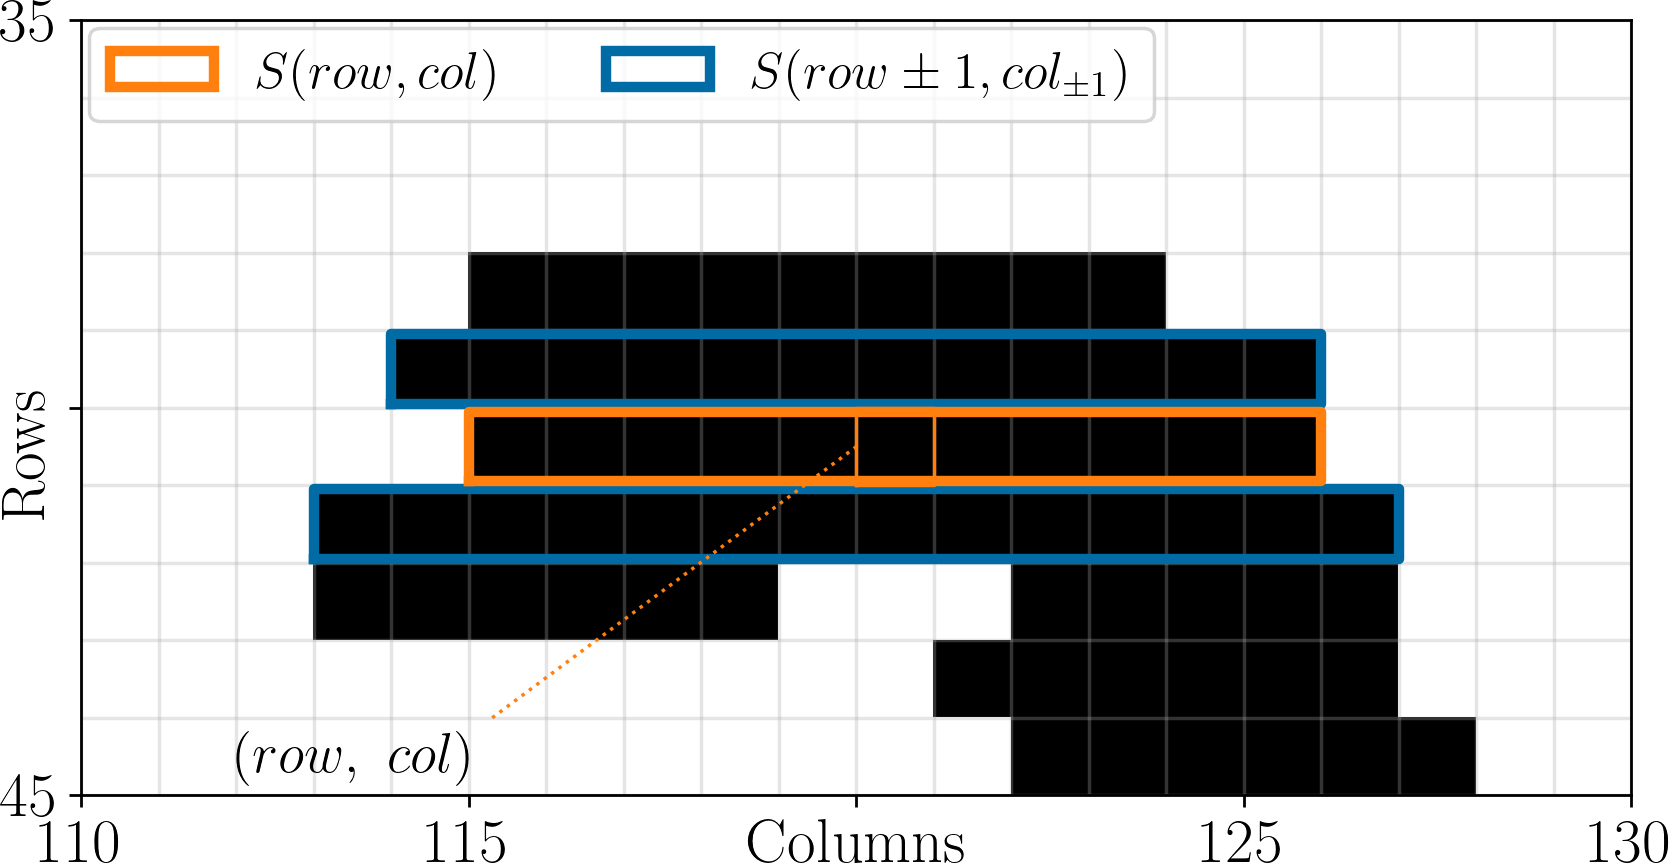
\includegraphics[width=\linewidth]{Images/Chap_5/low_confidence_segments_3.png}
        \caption{with $S(row\pm1, col_{\pm1})$}
        \label{fig:low_confidence_segments_3}
    \end{subfigure}
    \begin{subfigure}[t]{0.5\linewidth}
        \flushright
        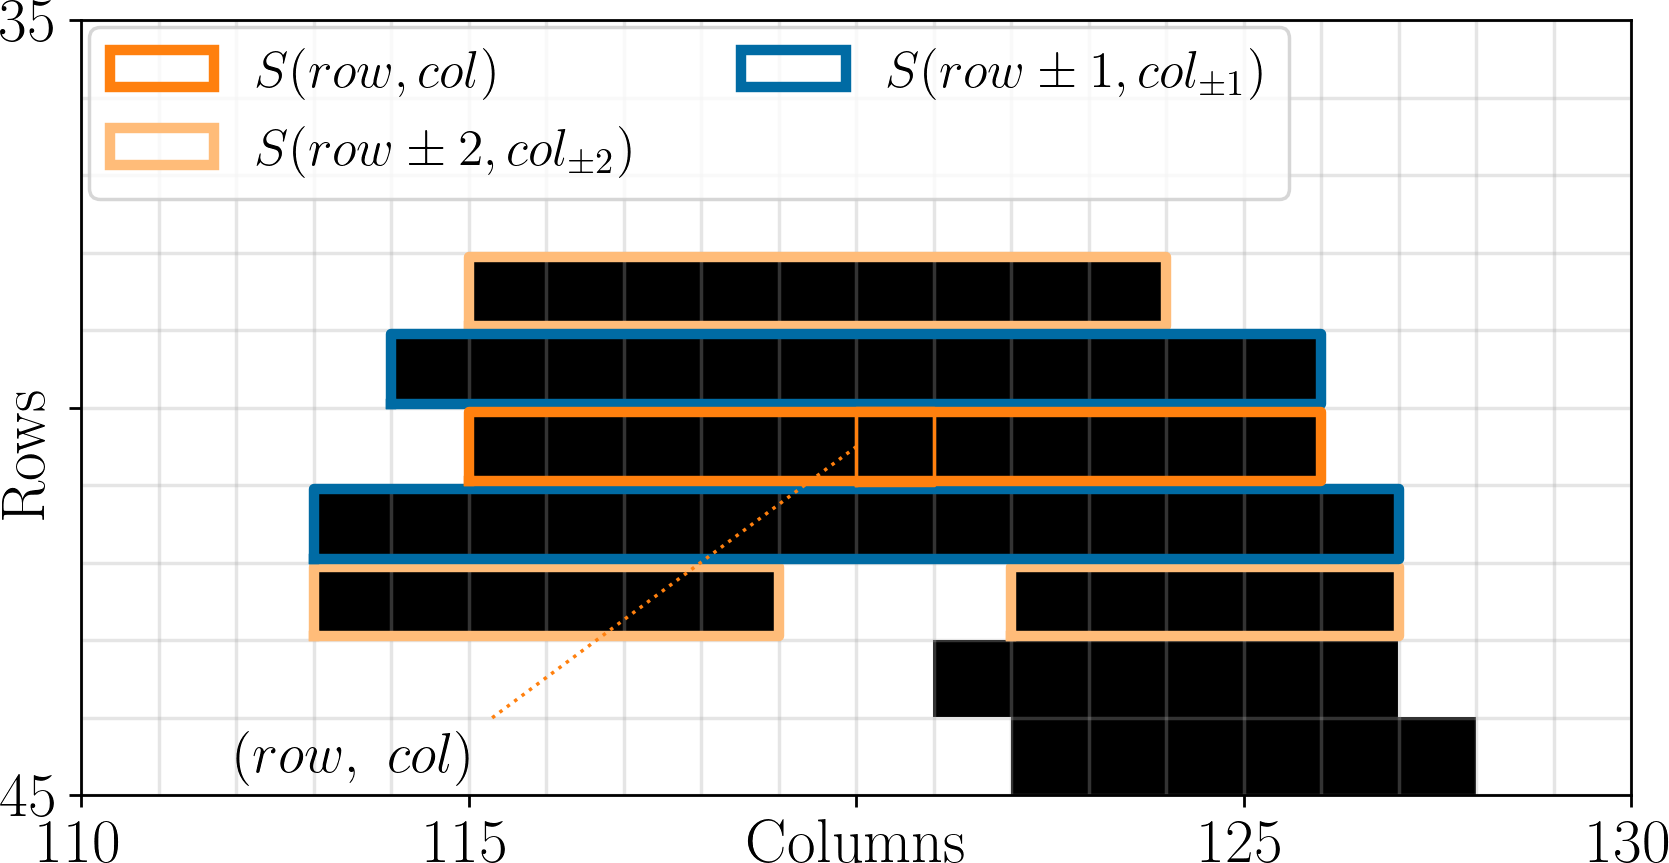
\includegraphics[width=\linewidth]{Images/Chap_5/low_confidence_segments_4.png}
        \caption{with $S(row\pm2, col_{\pm2})$}
        \label{fig:low_confidence_segments_4}
    \end{subfigure}\vspace*{0.3cm}
    \begin{subfigure}[t]{0.5\linewidth}
        \flushleft
        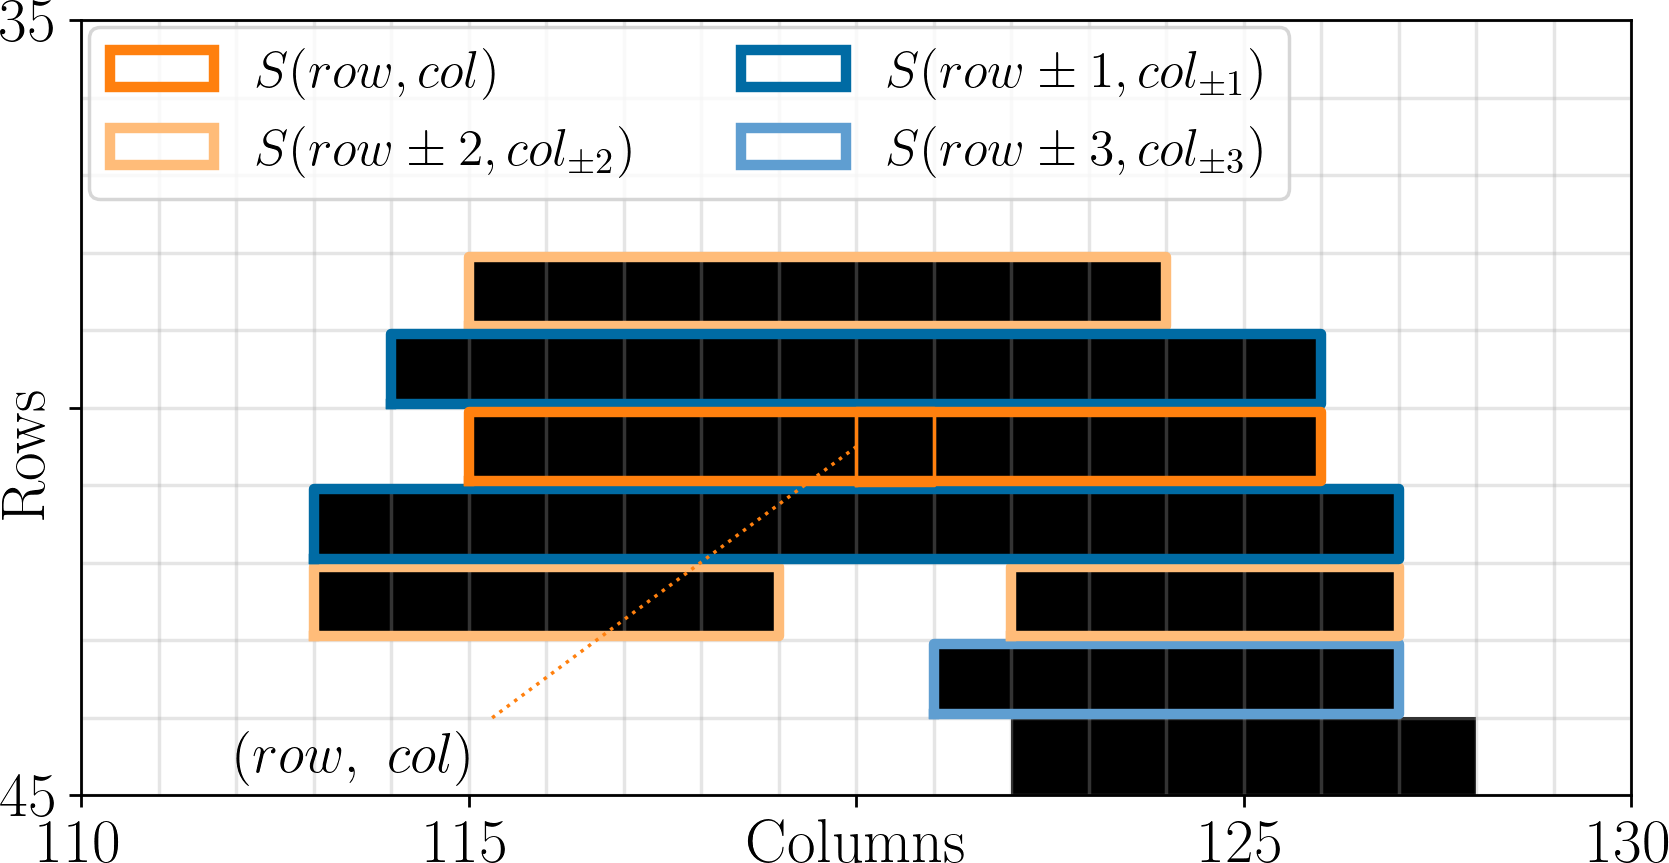
\includegraphics[width=\linewidth]{Images/Chap_5/low_confidence_segments_5.png}
        \caption{with $S(row\pm3, col_{\pm3})$}
        \label{fig:low_confidence_segments_5}
    \end{subfigure}
    \begin{subfigure}[t]{0.5\linewidth}
        \flushright
        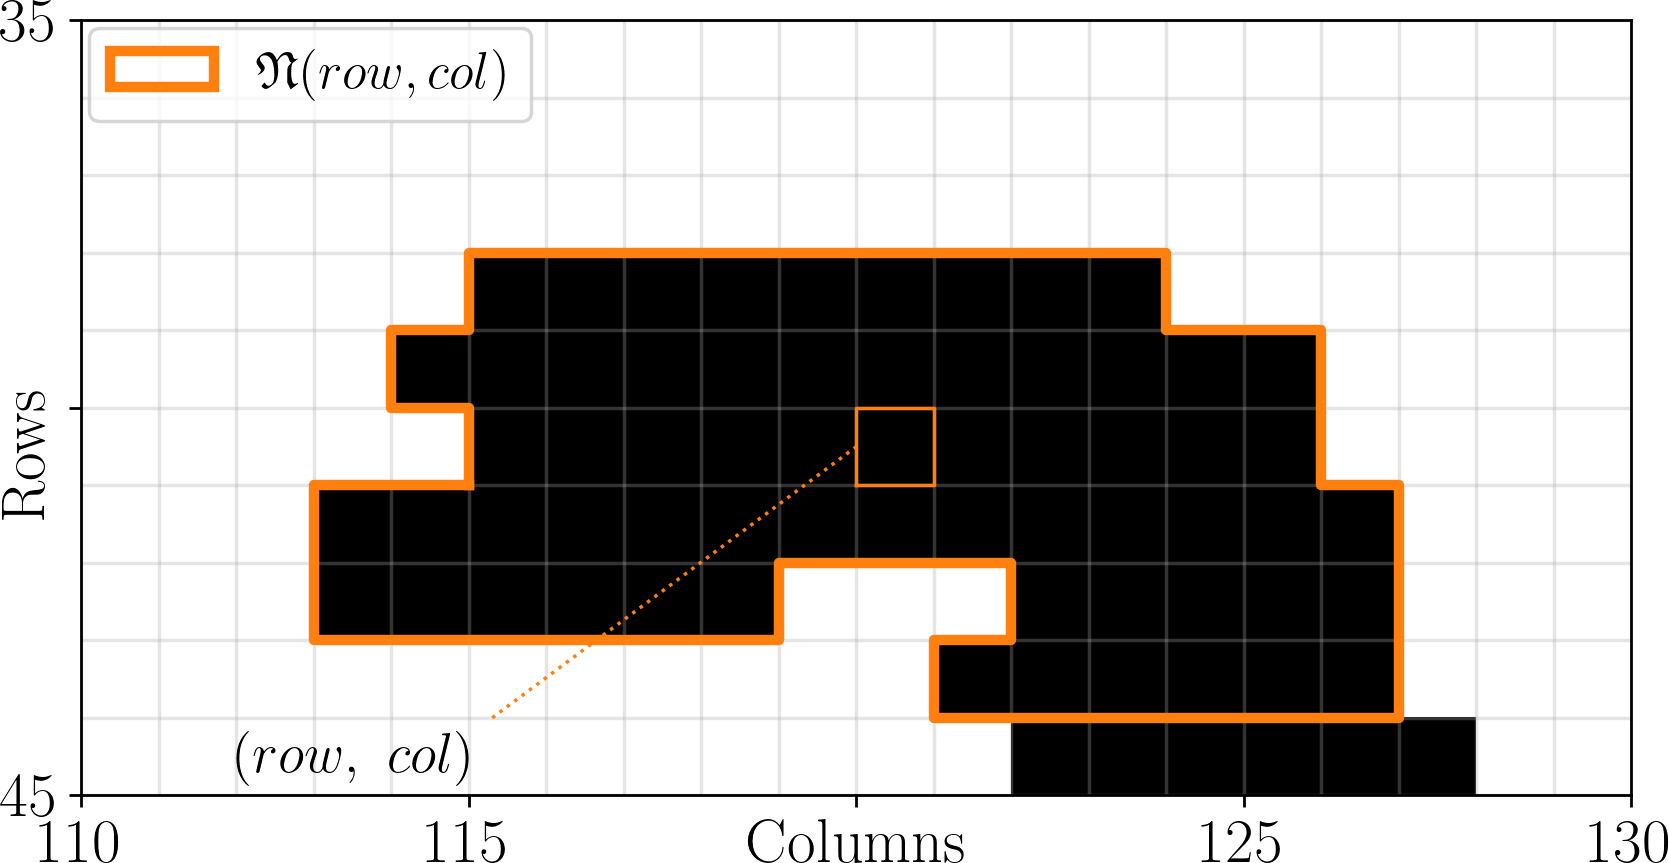
\includegraphics[width=\linewidth]{Images/Chap_5/low_confidence_segments_6.png}
        \caption{Resulting neighboring $\N(\rowcol)$}
        \label{fig:low_confidence_segments_6}
    \end{subfigure}
    \caption{Segments $S(\rowcol)$ and neighboring $\N(\rowcol)$. The image is an extract of the binary mask from \Cref{fig:ambiguity_mask_cones}, where low confidence pixels appear in black and high confidence pixels appear in white. \subref{fig:low_confidence_segments_1}: low confidence pixel $\rowcol$. From \subref{fig:low_confidence_segments_2} to \subref{fig:low_confidence_segments_5}: segment $S(row, ~ col)$ and adjacent segments over $3$ rows above and below. \subref{fig:low_confidence_segments_6}: resulting neighboring $\N(\rowcol)$.}
    \label{fig:low_confidence_segments}
\end{figure}

The value of the regularized interval $I^{reg}_\alpha$ of $(\rowcol)$ is obtained by consensus between the confidence intervals of $\N(\rowcol)$. Its upper and lower bounds are respectively the $q$\ith quantile of upper bounds of $\N(\rowcol)$ and the $(1-q)$\ith quantile of lower bounds of $\N(\rowcol)$:
\begin{align}
    I^{reg}_\alpha=[&\mathcal{Q}_{1-q}(\{\underline{I}_\alpha(r,~c)~|~(r,~c)\in\N(\rowcol)\}),\nonumber\\
    &\mathcal{Q}_q(\{\overline{I}_\alpha(r,~c)~|~(r,~c)\in\N(\rowcol)\})]\label{eq:quantile_reg}
\end{align}
where $\mathcal{Q}_q$ refers to the $q$\ith quantile of a set. In practice, we use $q=90\%$. This way, the lower bound of $I^{reg}_\alpha$ is lower than $90\%$ of lower bounds of intervals in $\N(\rowcol)$, and its upper bound is larger than $90\%$ of upper bounds of intervals in $\N(\rowcol)$. \Cref{fig:intervals_ambiguous_row_240,fig:intervals_ambiguous_row_290} present confidence intervals without and with regularization, for the same rows as in \Cref{fig:intervals_ambiguous_row_80_180,fig:intervals_ambiguous_row_240_290}.

\begin{remark}
    It does not necessarily mean that $I^{reg}_\alpha$ includes $90\%$ of intervals of $\N(\rowcol)$. Indeed, there can be intervals whose lower bound is greater than the $(1-q)$\ith quantile of lower bounds while also being greater than the $q$\ith quantile of upper bounds. The intervals will then overlap while not being included in one another.
\end{remark}

We can notice that it is possible, although unlikely, that the $q$\ith quantile of the upper bounds of $\N(\rowcol)$ is lesser than the predicted disparity $\tilde{d}(\rowcol)$ (or similarly, the $(1-q)$\ith quantile of lower bounds can be greater than $\tilde{d}(\rowcol)$). In that case, in order to ensure the coherence of the predicted disparity with the confidence intervals, the bounds of the intervals are extended until they include $\tilde{d}$.
\begin{figure}
    \centering
    \begin{subfigure}[t]{\linewidth}
        \centering
        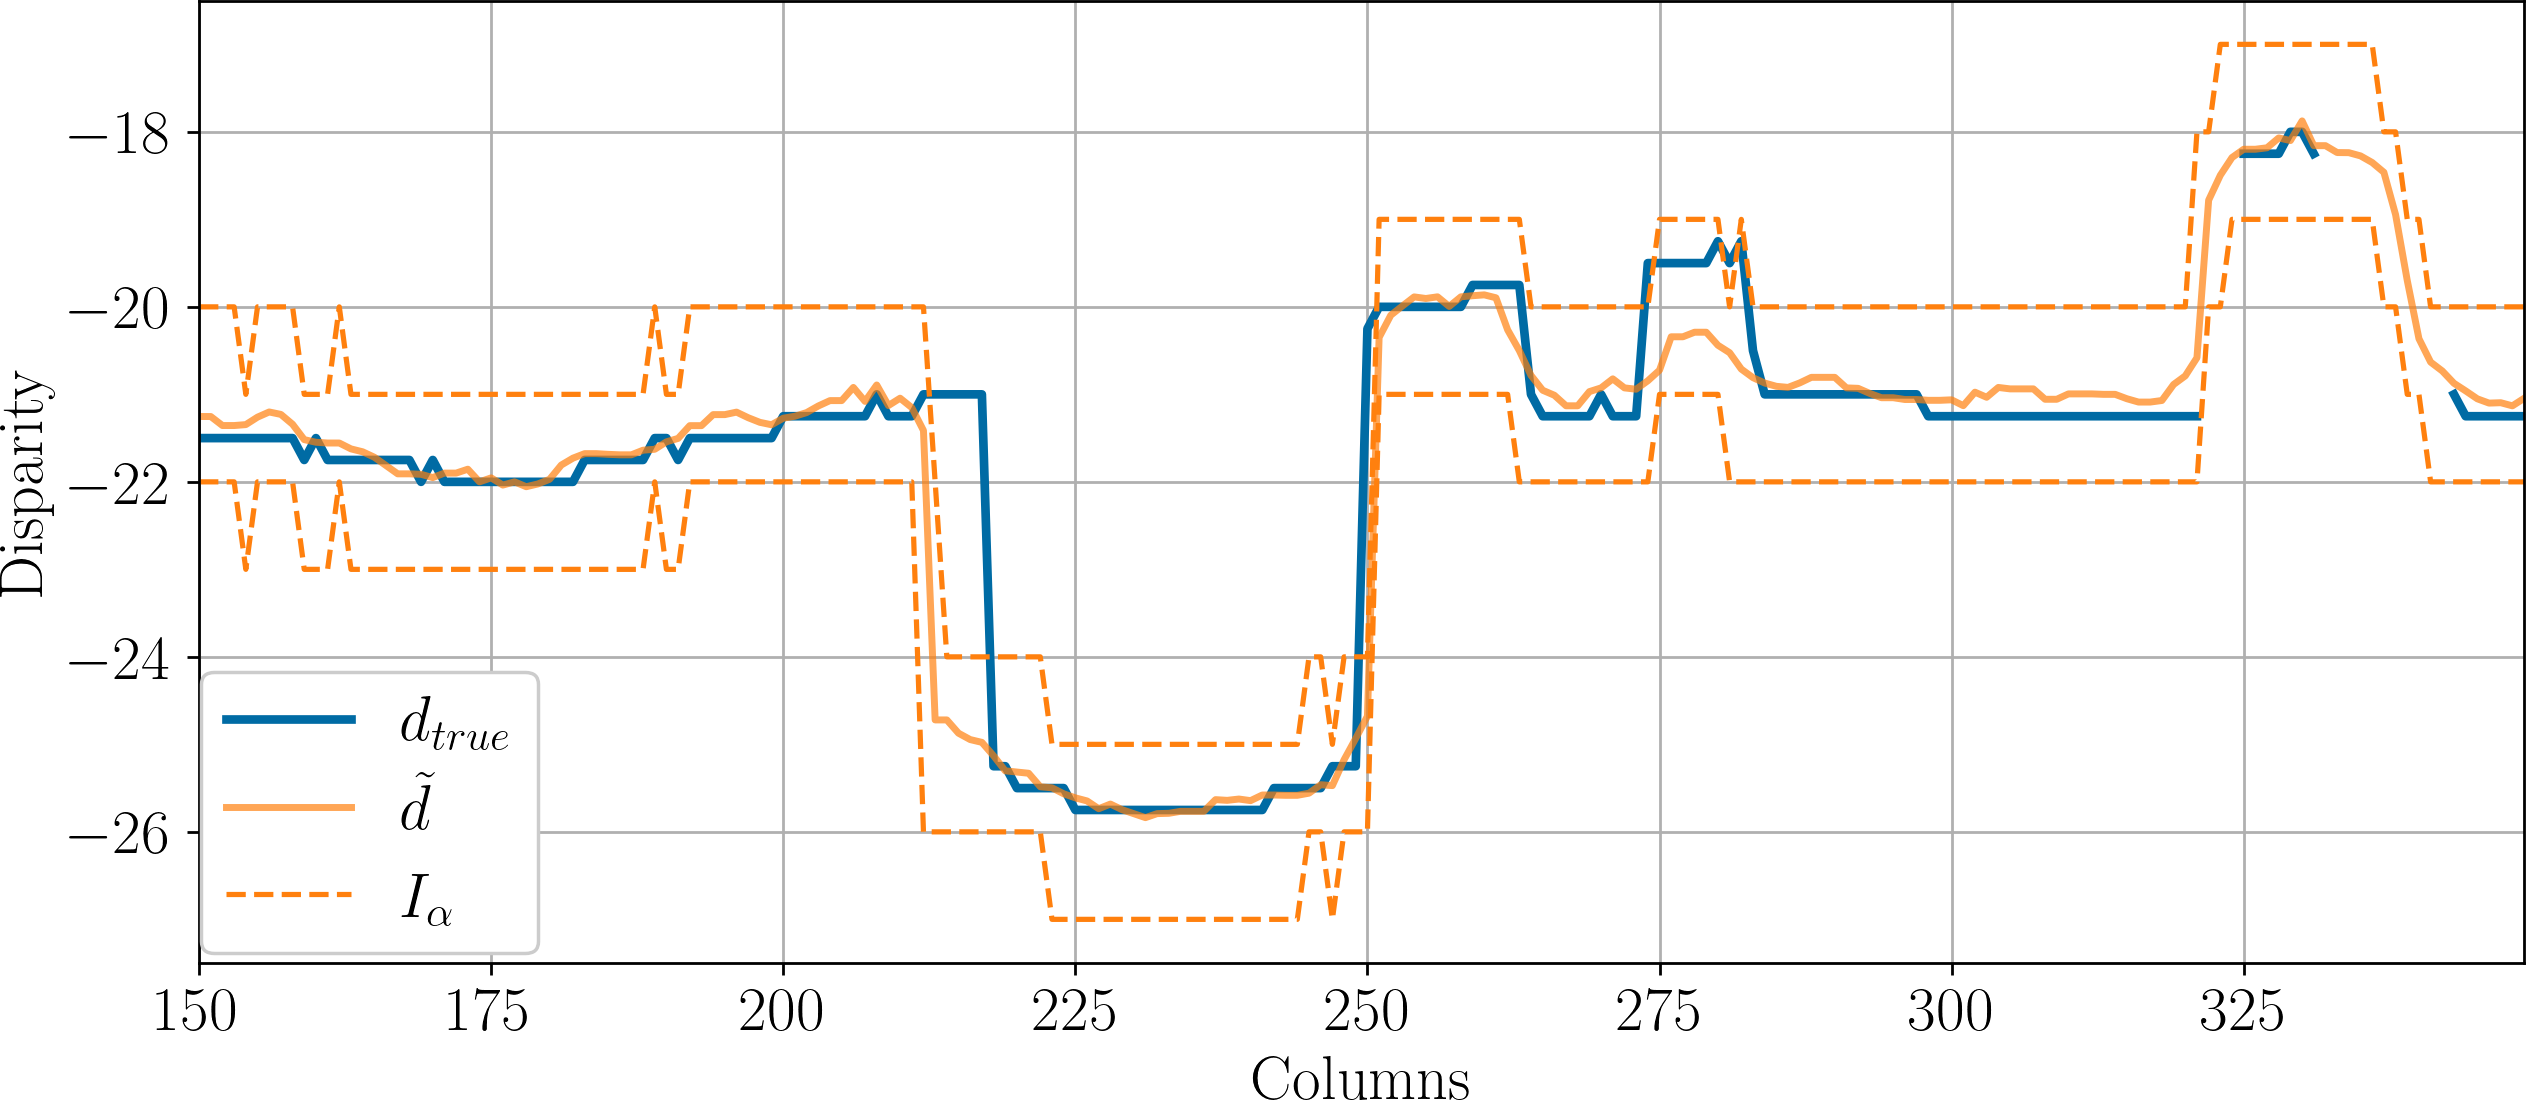
\includegraphics[width=\linewidth]{Images/Chap_5/intervals_ambiguous_area_row_80_1.png}
        \caption{$I_\alpha$ without regularization in low confidence areas}
        \label{fig:intervals_ambiguous_row_80_1}
    \end{subfigure}\hfill
    \begin{subfigure}[t]{\linewidth}
        \centering
        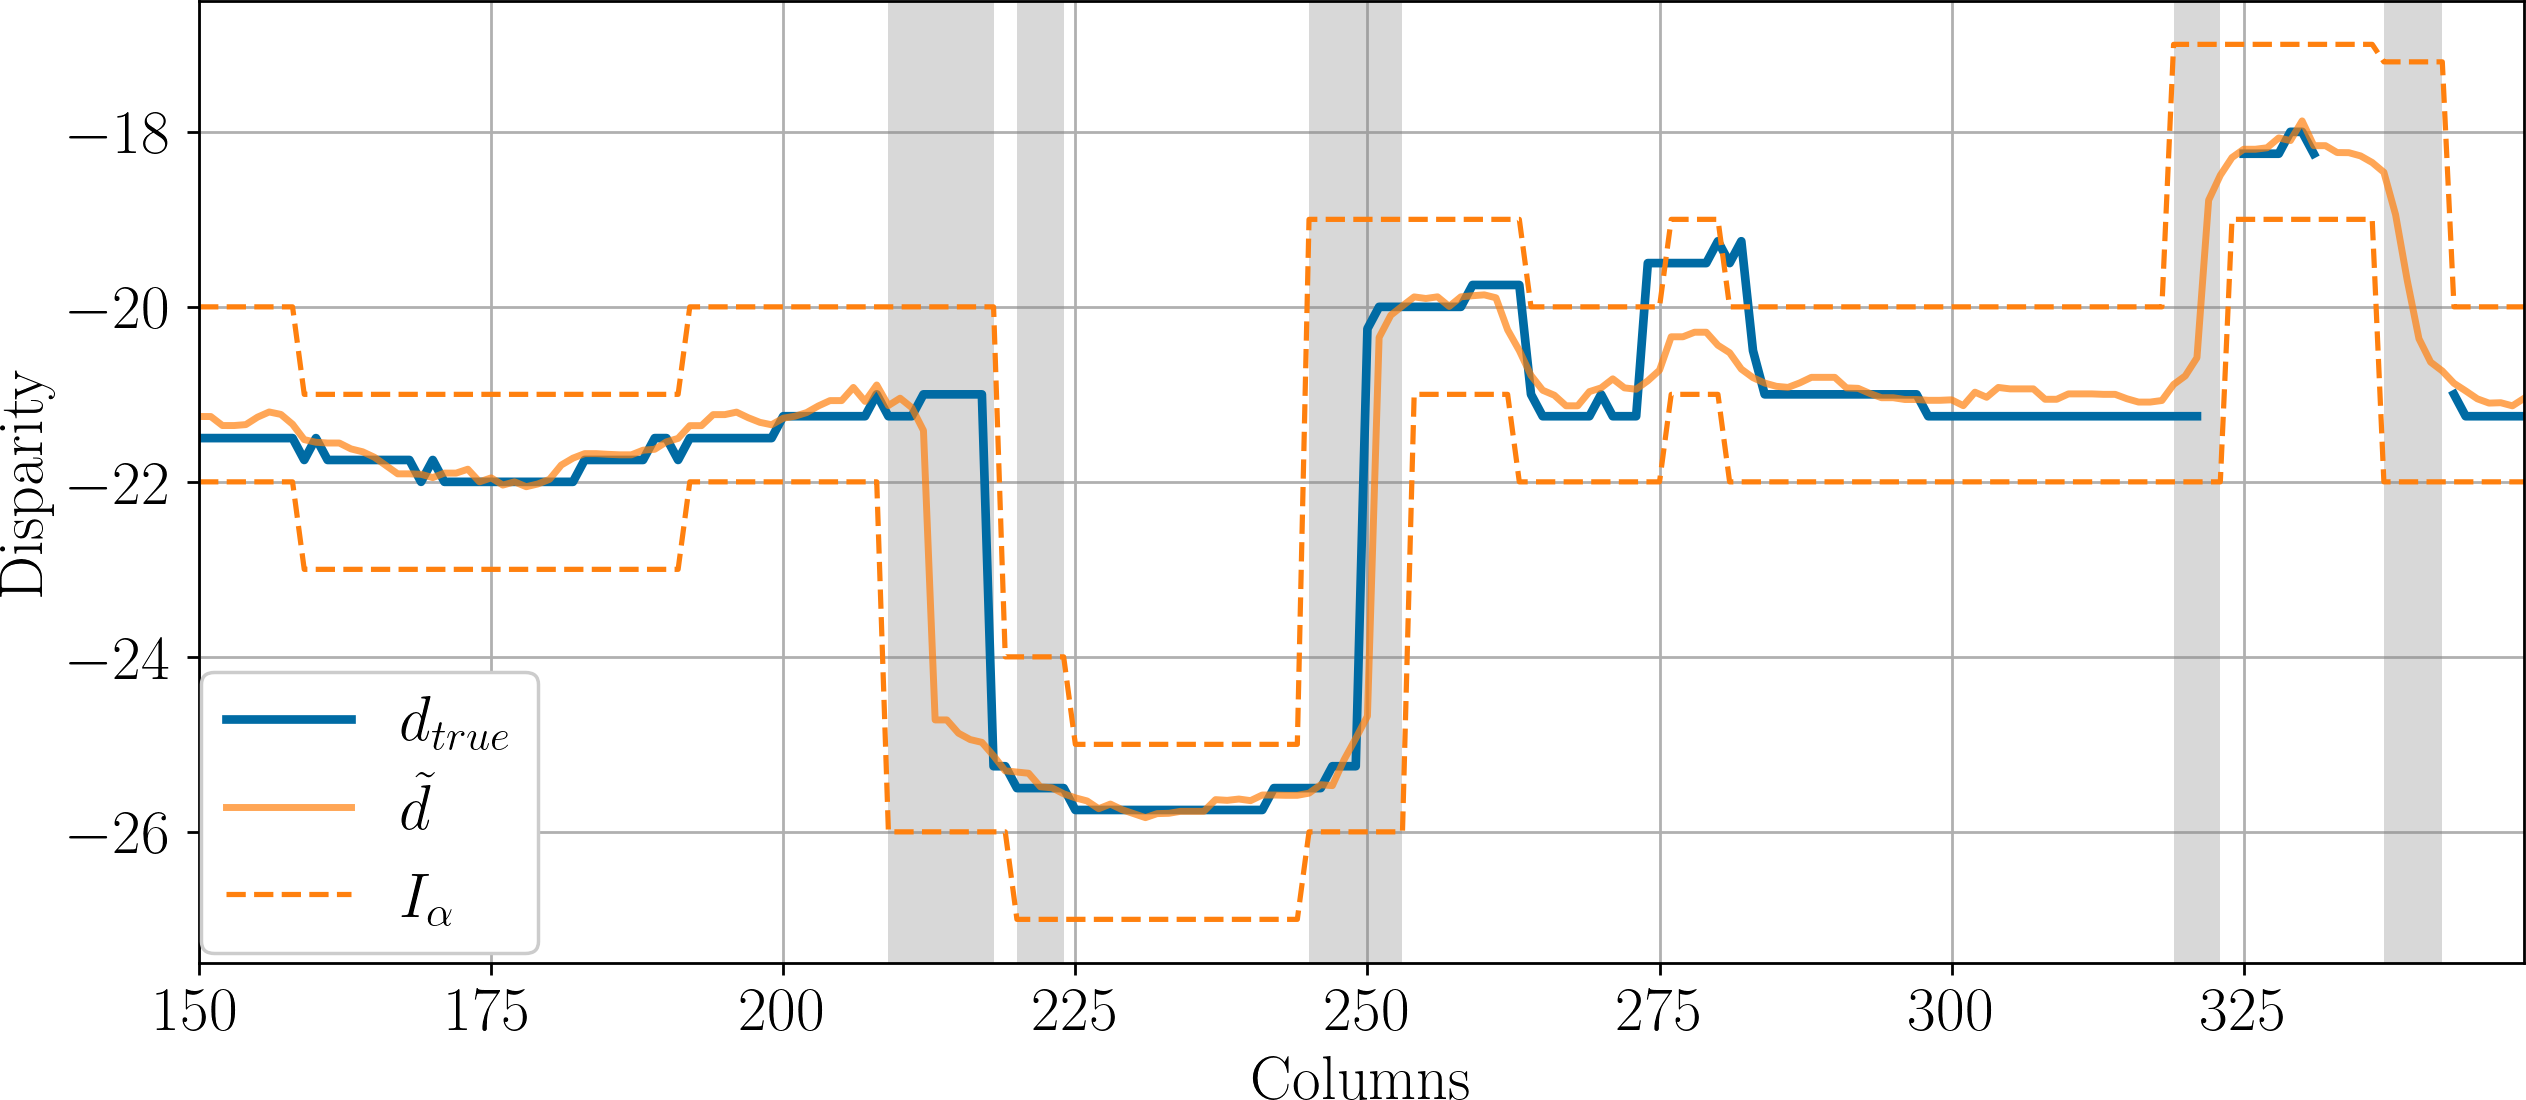
\includegraphics[width=\linewidth]{Images/Chap_5/intervals_ambiguous_area_row_80_2.png}
        \caption{$I_\alpha$ with regularization in low confidence areas}
        \label{fig:intervals_ambiguous_row_80_2}
    \end{subfigure}
    \caption{$I_\alpha$ with and without regularization in low confidence area, for row $80$ of the image of \Cref{fig:cones_with_rows}. The gray areas indicate low confidence areas.}
    \label{fig:intervals_ambiguous_row_80}
\end{figure}

\begin{figure}
    \centering
    \begin{subfigure}[t]{\linewidth}
        \centering
        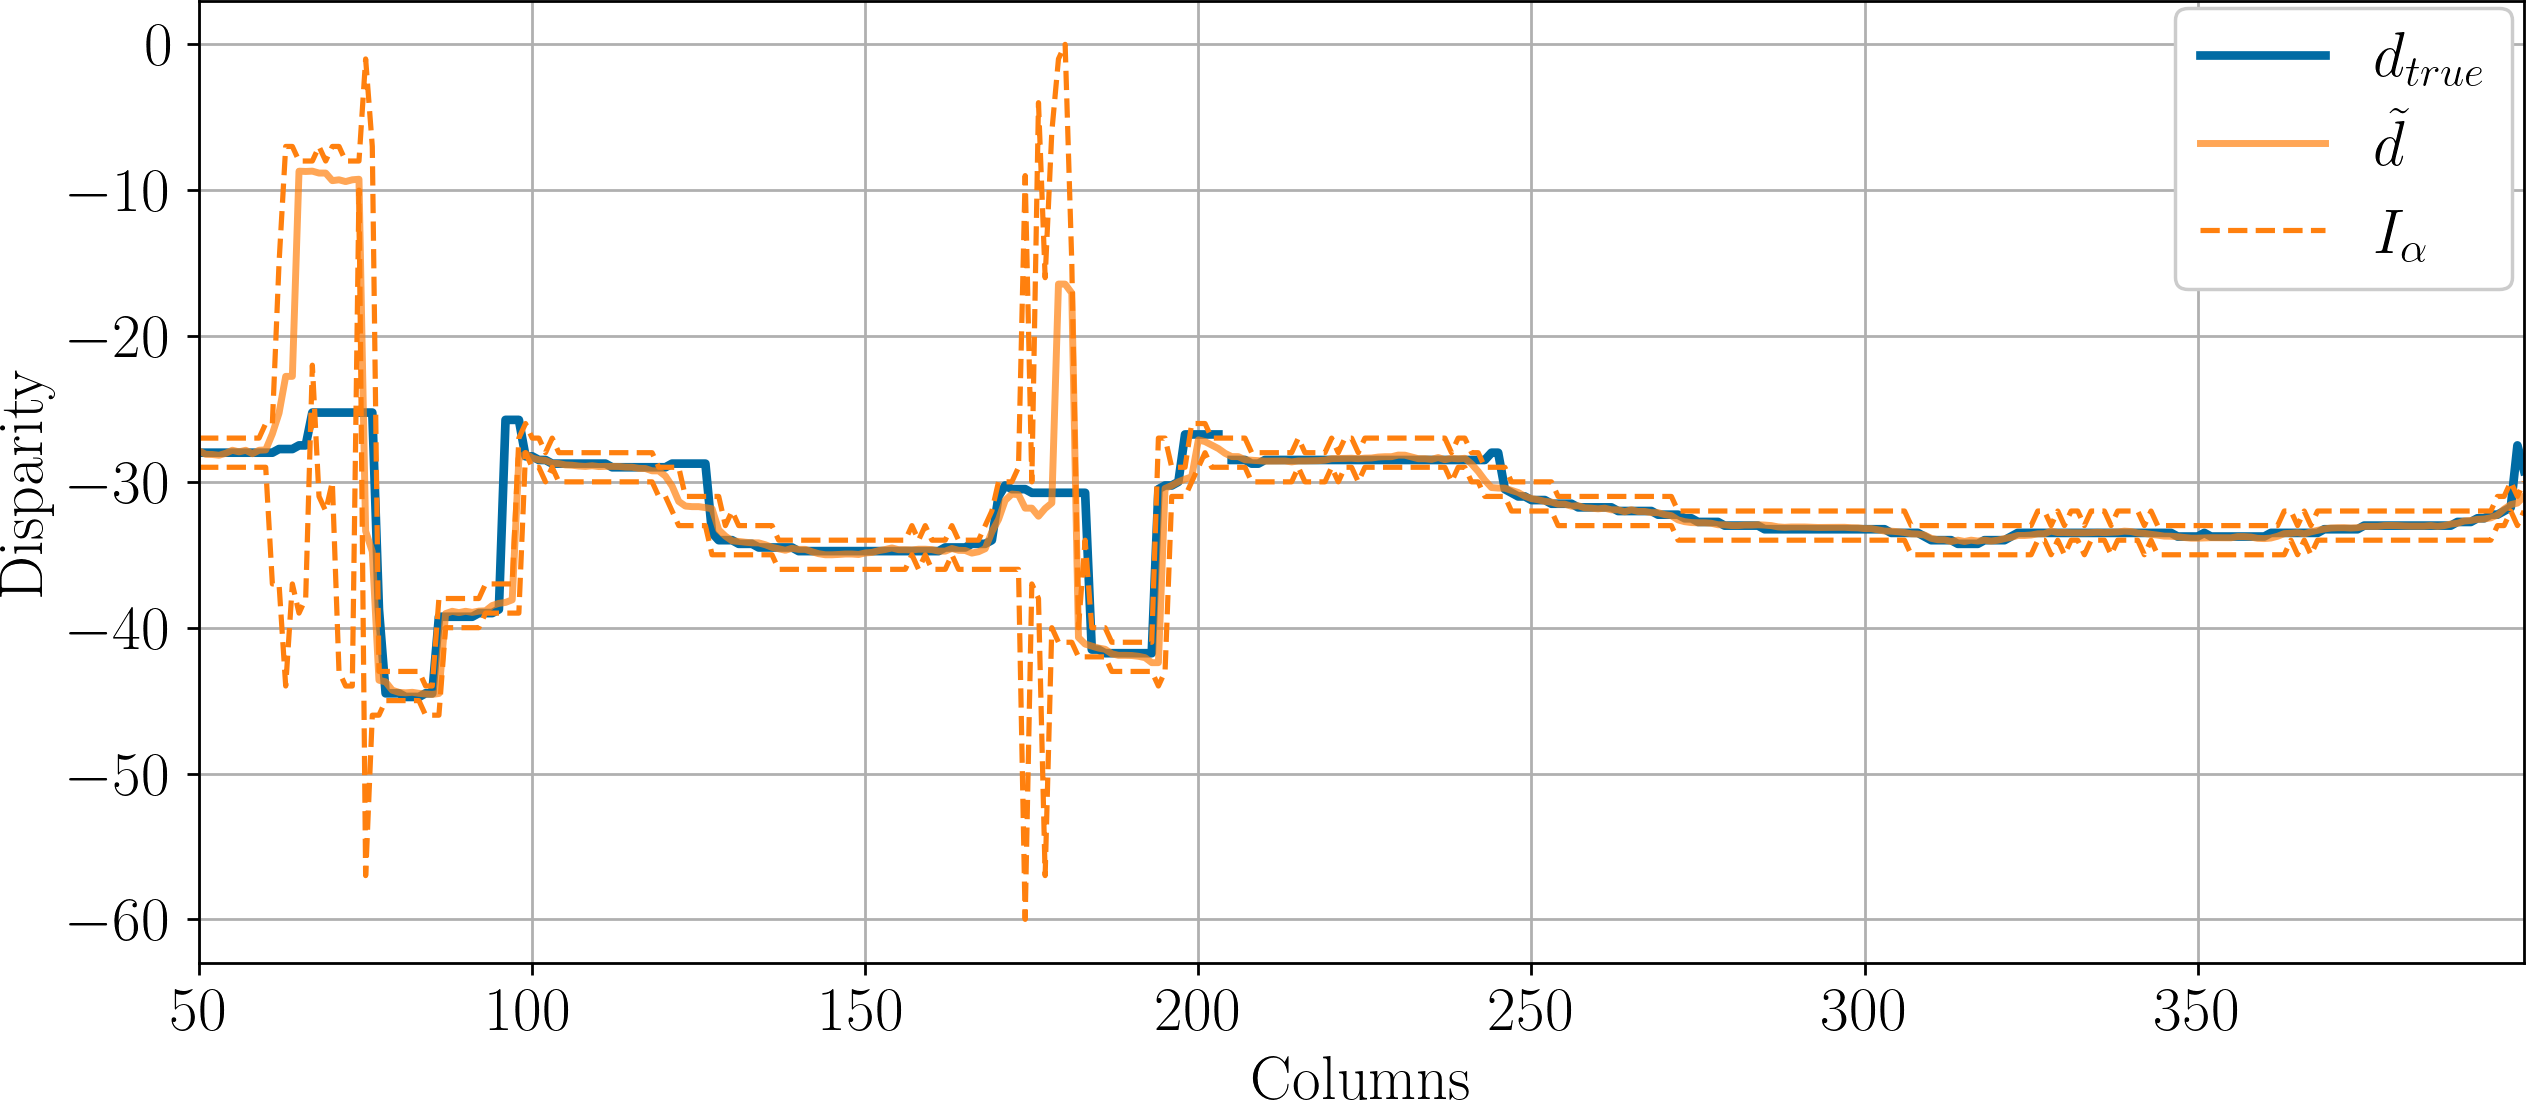
\includegraphics[width=\linewidth]{Images/Chap_5/intervals_ambiguous_area_row_180_1.png}
        \caption{$I_\alpha$ without regularization in low confidence areas}
        \label{fig:intervals_ambiguous_row_180_1}
    \end{subfigure}\hfill
    \begin{subfigure}[t]{\linewidth}
        \centering
        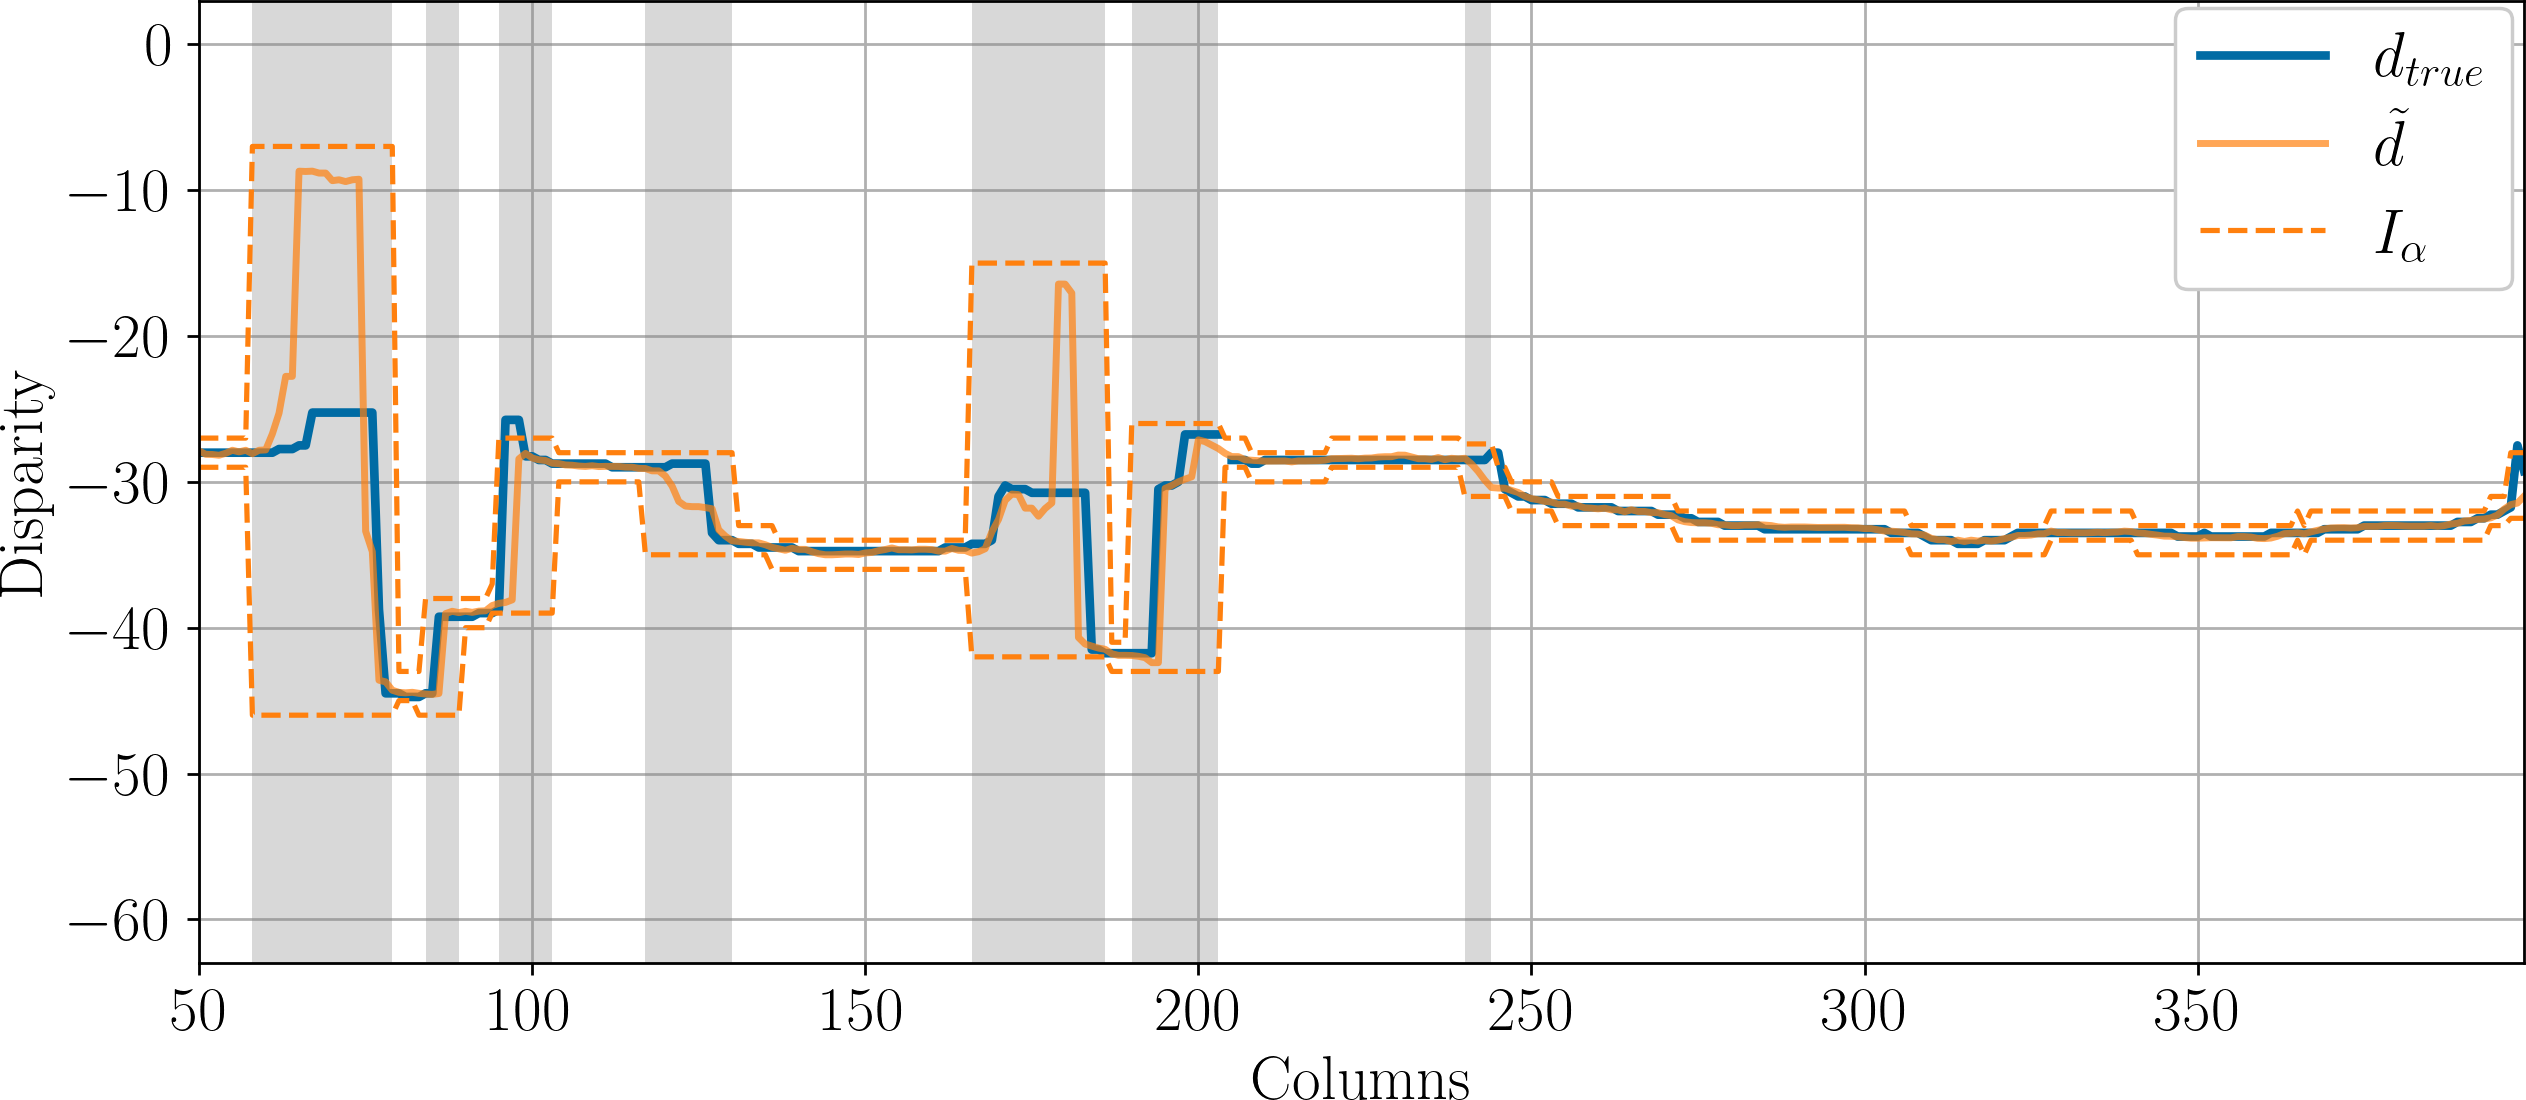
\includegraphics[width=\linewidth]{Images/Chap_5/intervals_ambiguous_area_row_180_2.png}
        \caption{$I_\alpha$ with regularization in low confidence areas}
        \label{fig:intervals_ambiguous_row_180_2}
    \end{subfigure}
    \caption{$I_\alpha$ with and without regularization in low confidence area, for row $180$ of the image of \Cref{fig:cones_with_rows}. The gray areas indicate low confidence areas.}
    \label{fig:intervals_ambiguous_row_180}
\end{figure}

\begin{figure}
    \centering
    \begin{subfigure}[t]{\linewidth}
        \centering
        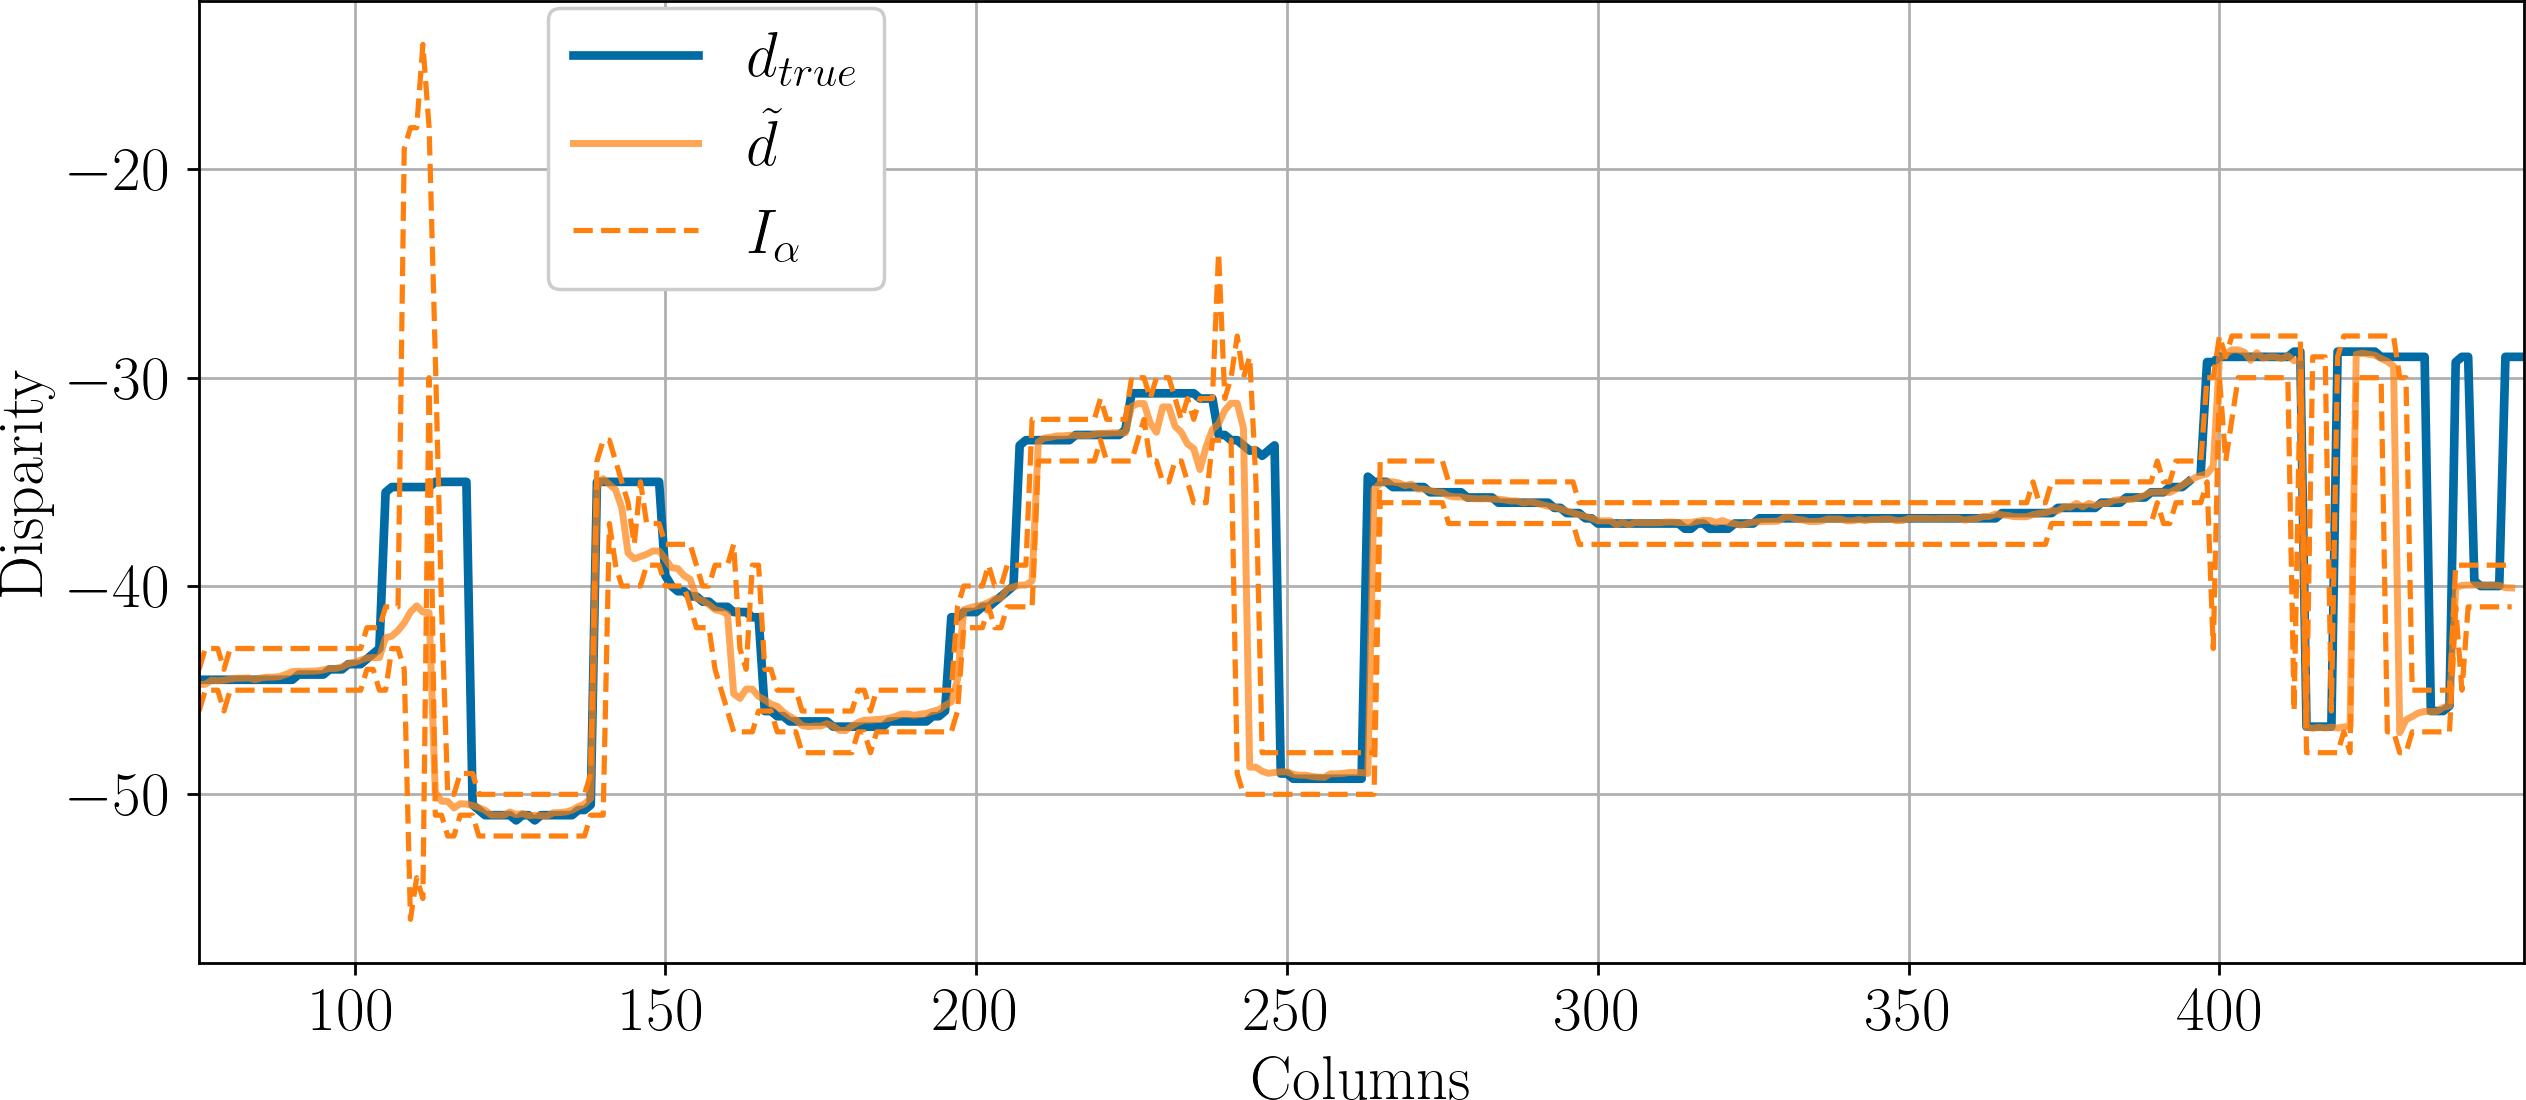
\includegraphics[width=\linewidth]{Images/Chap_5/intervals_ambiguous_area_row_240_1.png}
        \caption{$I_\alpha$ without regularization in low confidence areas}
        \label{fig:intervals_ambiguous_row_240_1}
    \end{subfigure}\hfill
    \begin{subfigure}[t]{\linewidth}
        \centering
        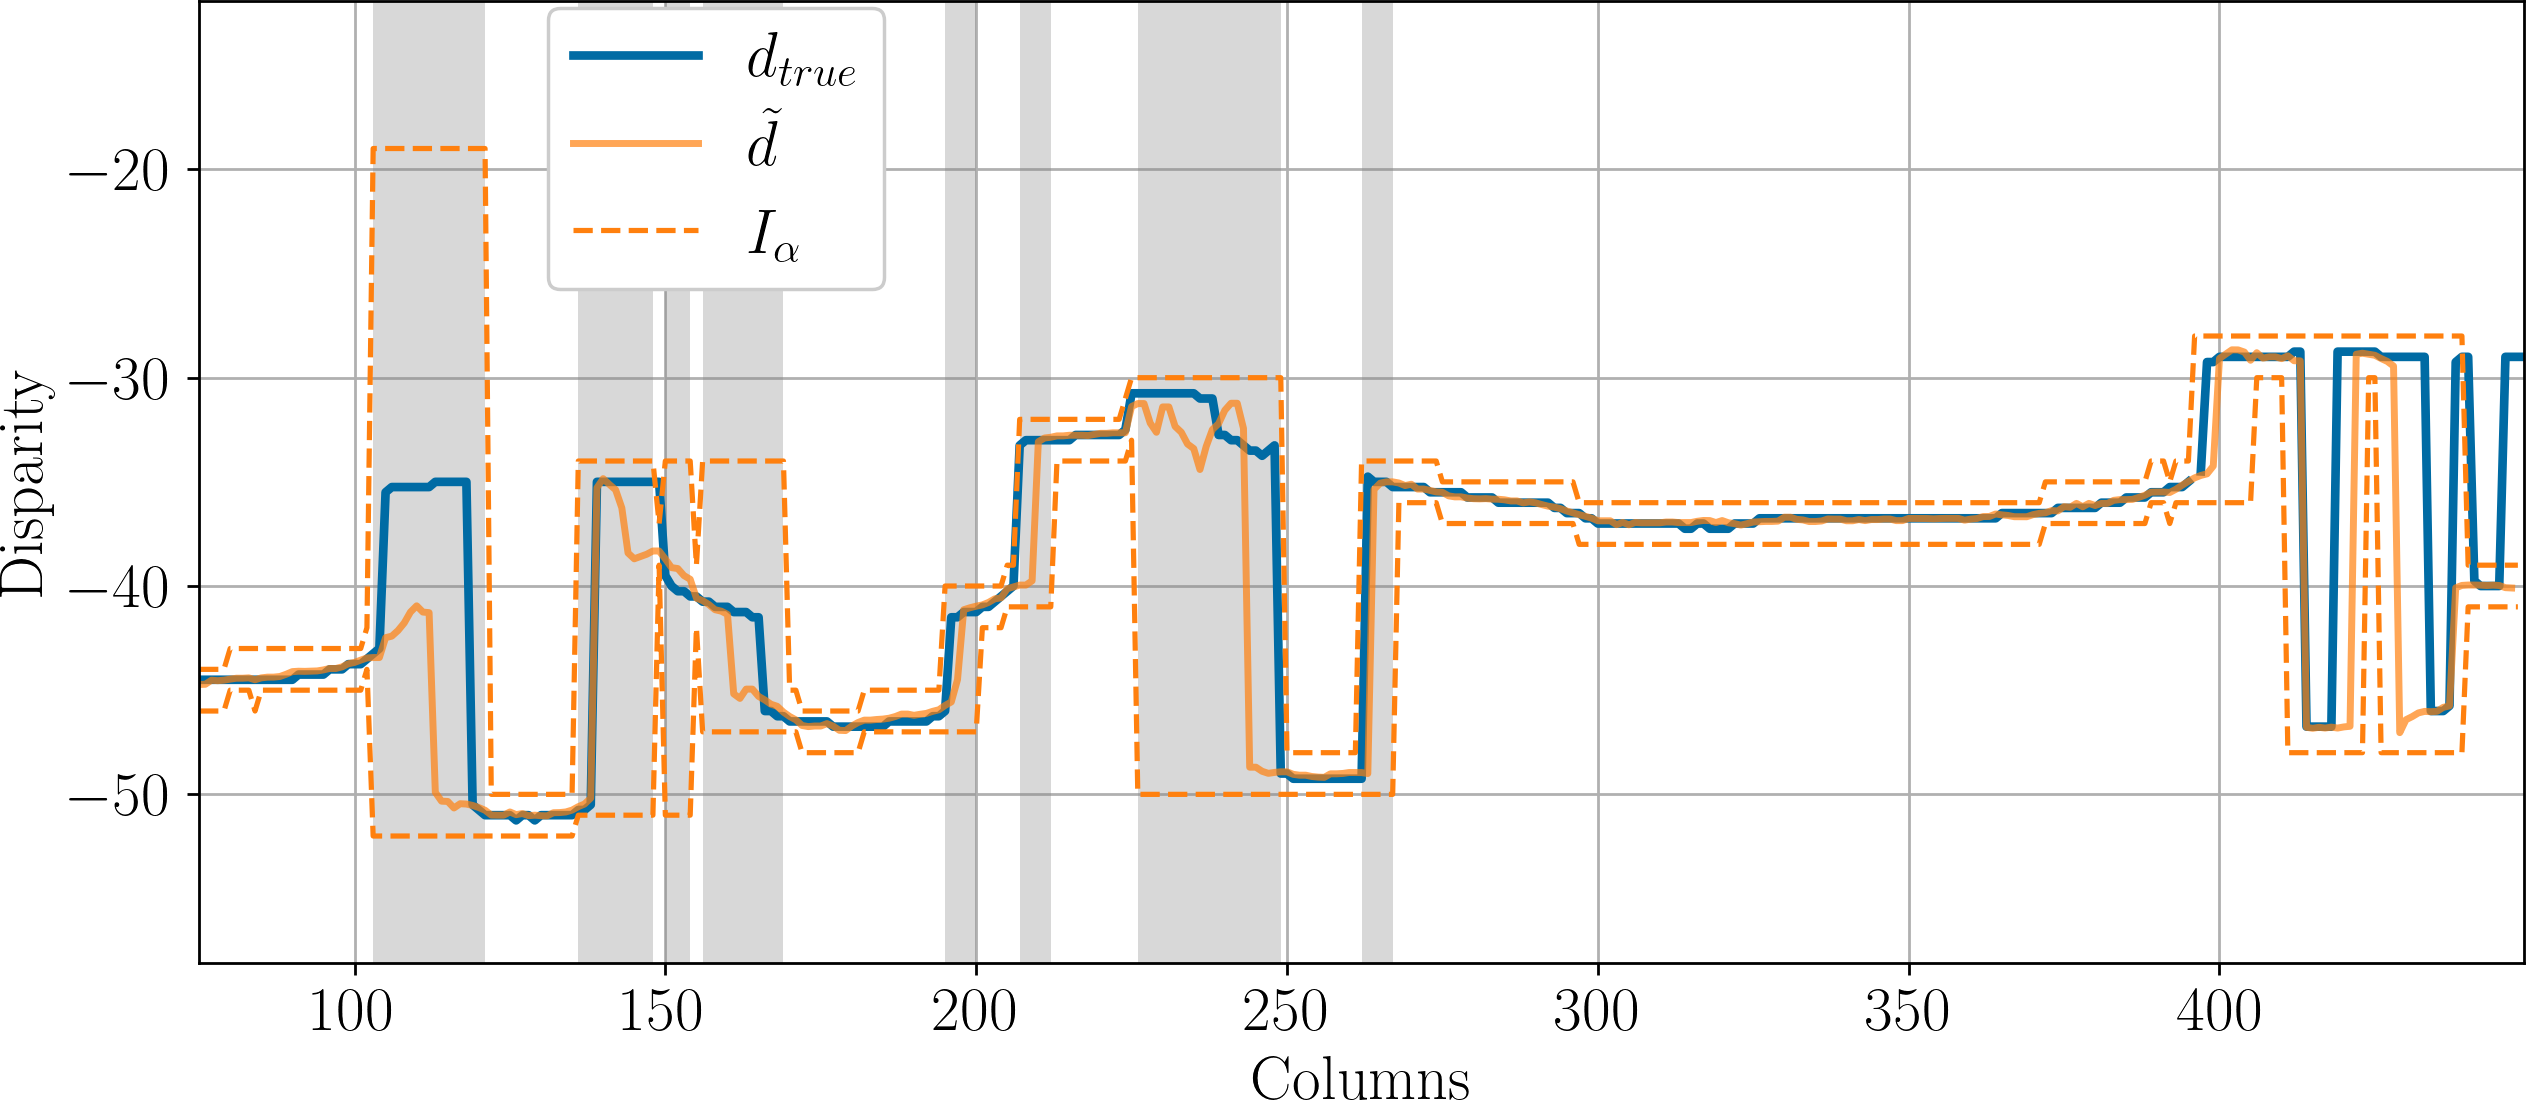
\includegraphics[width=\linewidth]{Images/Chap_5/intervals_ambiguous_area_row_240_2.png}
        \caption{$I_\alpha$ with regularization in low confidence areas}
        \label{fig:intervals_ambiguous_row_240_2}
    \end{subfigure}
    \caption{$I_\alpha$ with and without regularization in low confidence area, for row $240$ of the image of \Cref{fig:cones_with_rows}. The gray areas indicate low confidence areas.}
    \label{fig:intervals_ambiguous_row_240}
\end{figure}

\begin{figure}
    \centering
    \begin{subfigure}[t]{\linewidth}
        \centering
        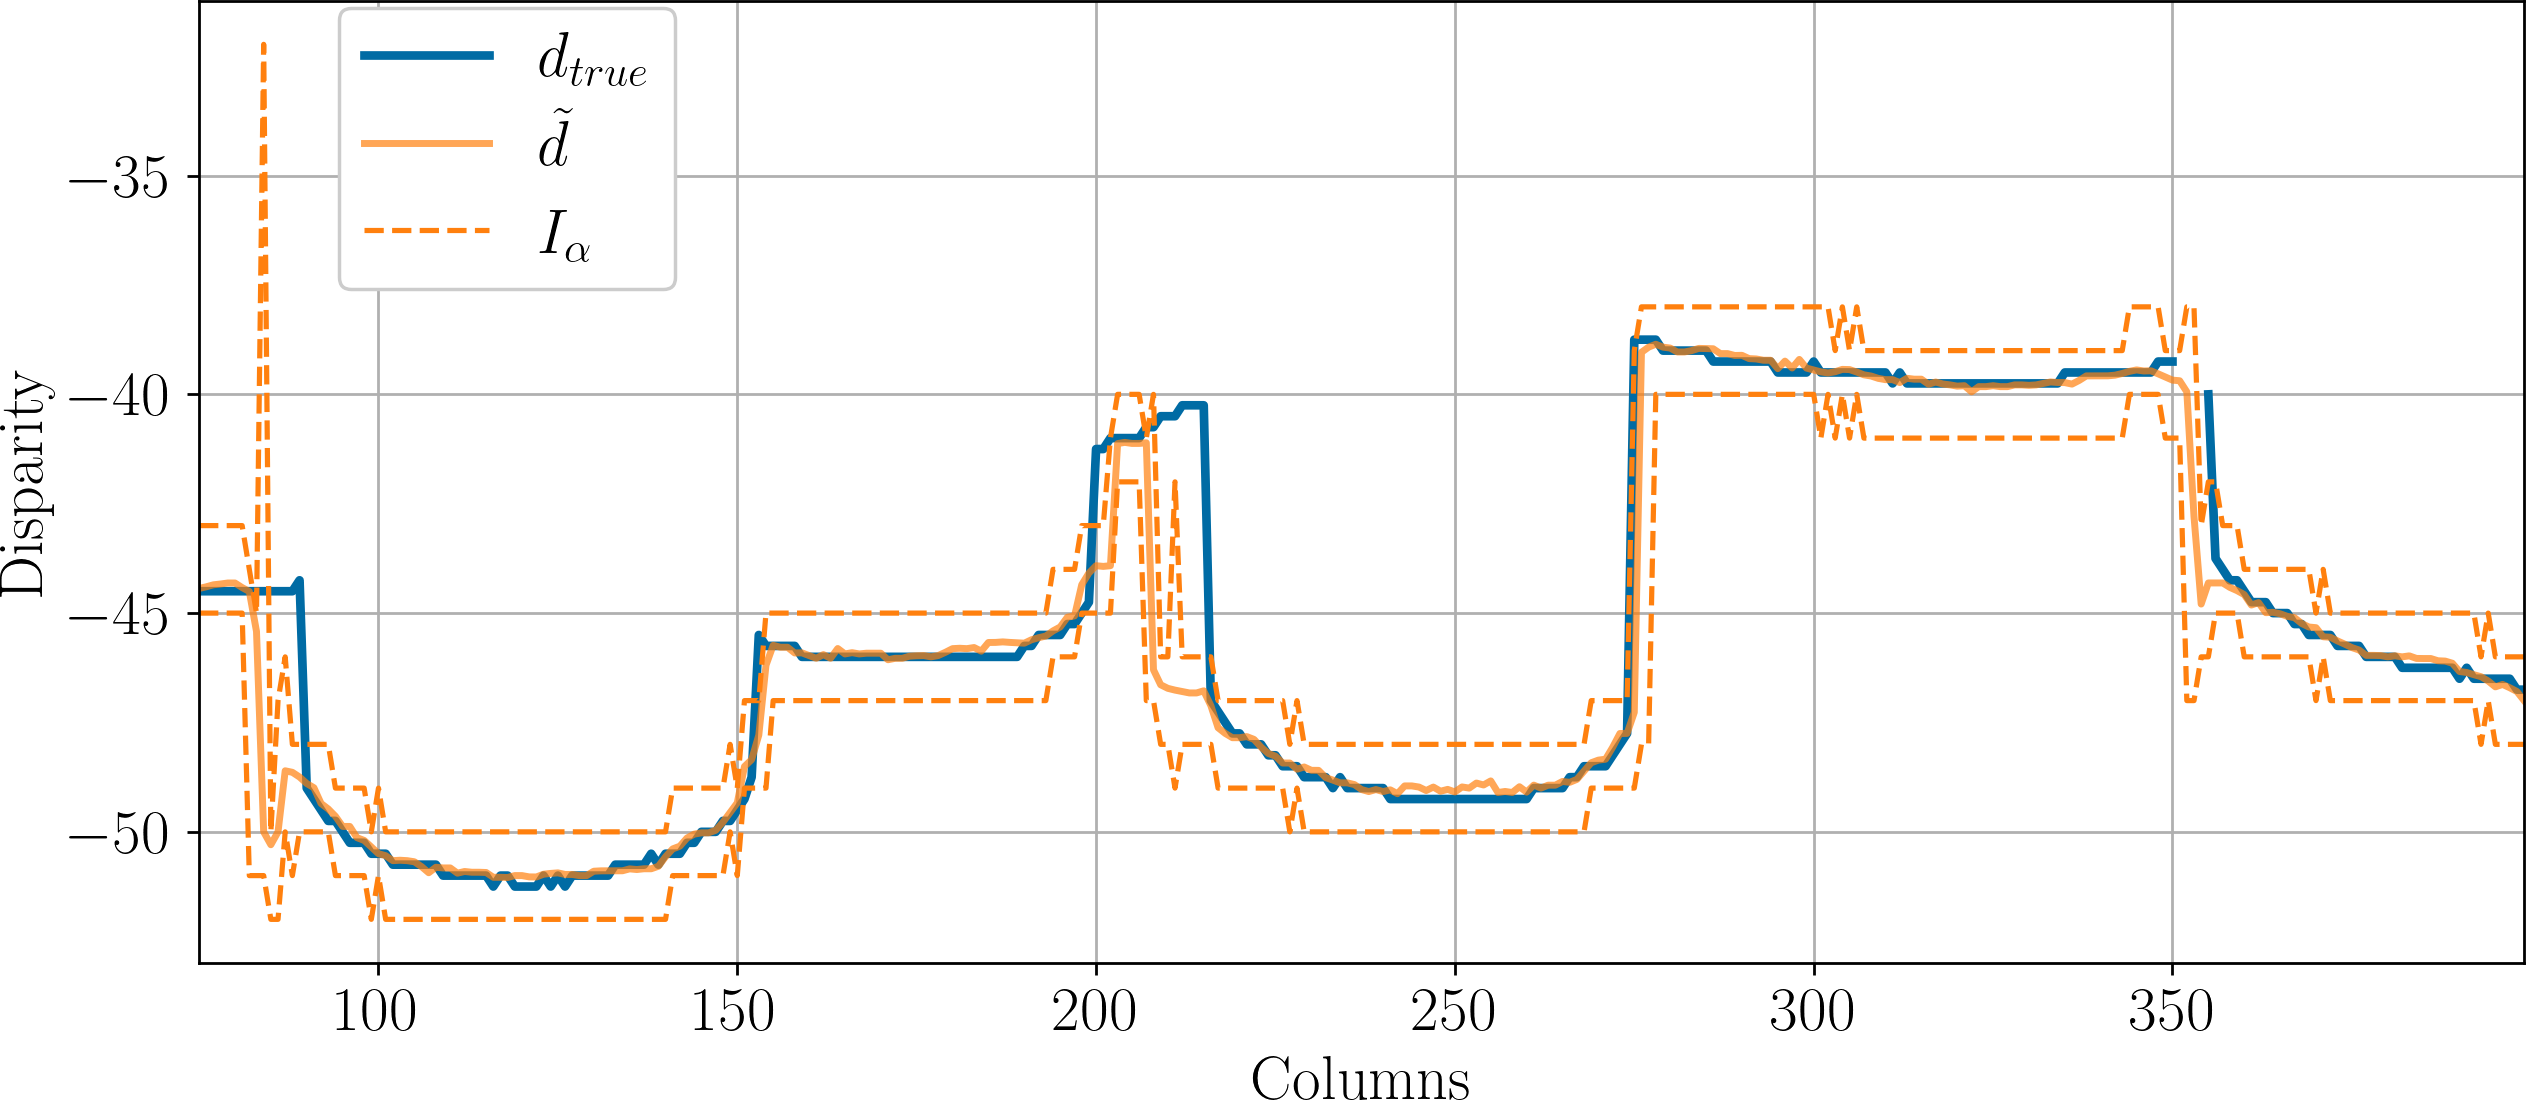
\includegraphics[width=\linewidth]{Images/Chap_5/intervals_ambiguous_area_row_290_1.png}
        \caption{$I_\alpha$ without regularization in low confidence areas}
        \label{fig:intervals_ambiguous_row_290_1}
    \end{subfigure}\hfill
    \begin{subfigure}[t]{\linewidth}
        \centering
        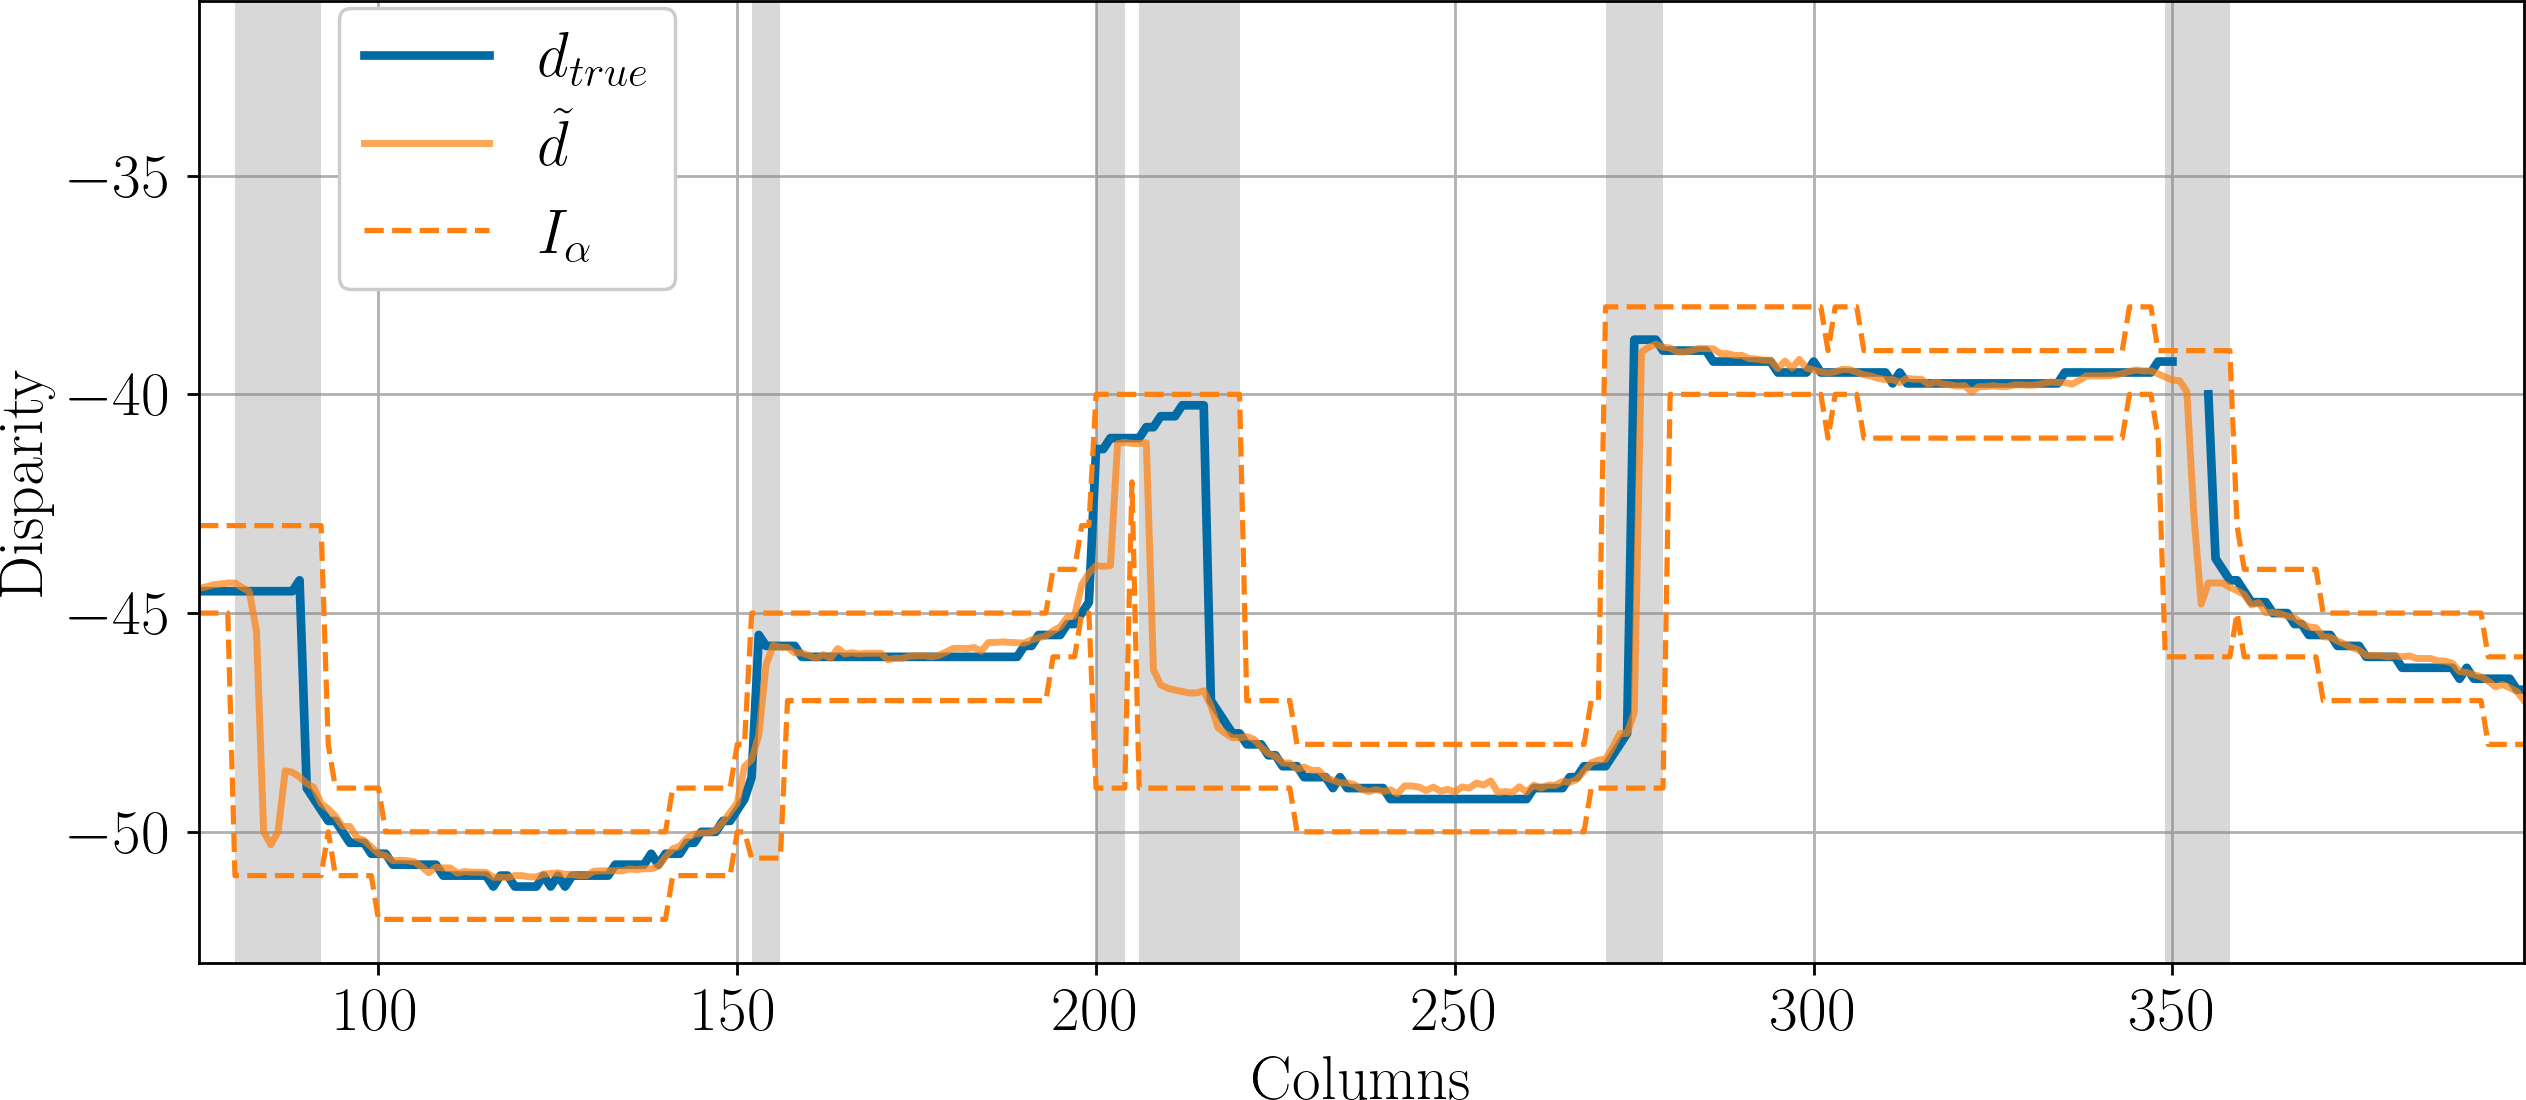
\includegraphics[width=\linewidth]{Images/Chap_5/intervals_ambiguous_area_row_290_2.png}
        \caption{$I_\alpha$ with regularization in low confidence areas}
        \label{fig:intervals_ambiguous_row_290_2}
    \end{subfigure}
    \caption{$I_\alpha$ with and without regularization in low confidence area, for row $290$ of the image of \Cref{fig:cones_with_rows}. The gray areas indicate low confidence areas.}
    \label{fig:intervals_ambiguous_row_290}
\end{figure}

Two pixels $(\rowcol)$ and $(row,~col')$ of $S(\rowcol)$ will have the same neighboring $\N(row,col)$. Therefore, they will also share the same value for their regularized interval $I^{reg}_\alpha$. This can be observed in \Cref{fig:intervals_ambiguous_row_80_2,fig:intervals_ambiguous_row_180_2,fig:intervals_ambiguous_row_240_2,fig:intervals_ambiguous_row_290_2}, where positions of low confidence pixels that are regularized are indicated using gray areas. 

In the following, we always regularize intervals in low confidence areas. We will thus refer to them simply as $I_\alpha$ instead of $I^{reg}_\alpha$, to simplify notations.

In theory, it is possible to perform the regularization of intervals before the filtering and refinement steps, but we chose to always regularize the intervals after those steps. This prevents outliers removed by the filtering step from influencing values of regularized intervals. \Cref{fig:intervals_ambiguous_row_80,fig:intervals_ambiguous_row_180,fig:intervals_ambiguous_row_240,fig:intervals_ambiguous_row_290} allow visualizing the impact of the regularization of intervals after the filtering and refinement steps. In \Cref{fig:intervals_ambiguous_row_80_2} near column $215$, we can see that the regularization allows to create correct confidence intervals. In \Cref{fig:intervals_ambiguous_row_180}, columns $70$ and $175$ also create correct intervals, in regions where the predicted disparity $\tilde{d}$ is far away from the ground truth. We can say that the intervals are (almost) as small as possible so as to both contain $\tilde{d}$ and the true disparity $d_{true}$, as they are necessarily constant in low confidence areas (gray areas in the figure). Column $175$ of \Cref{fig:intervals_ambiguous_row_180} also shows that filtering and regularization methods are able to discard outliers: bounds of non-regularized intervals reach values between $-60$ and $0$ near column $175$, while the bounds of regularized intervals stay between $-42$ and $-15$. However, this method is not perfect, as it sometimes overestimates the size of intervals as in \Cref{fig:intervals_ambiguous_row_290_2} near column $110$, or do not predict correct intervals at all, as observed around column $450$.

\begin{figure}
    \centering
    \begin{subfigure}[t]{0.49\linewidth}
        \centering
        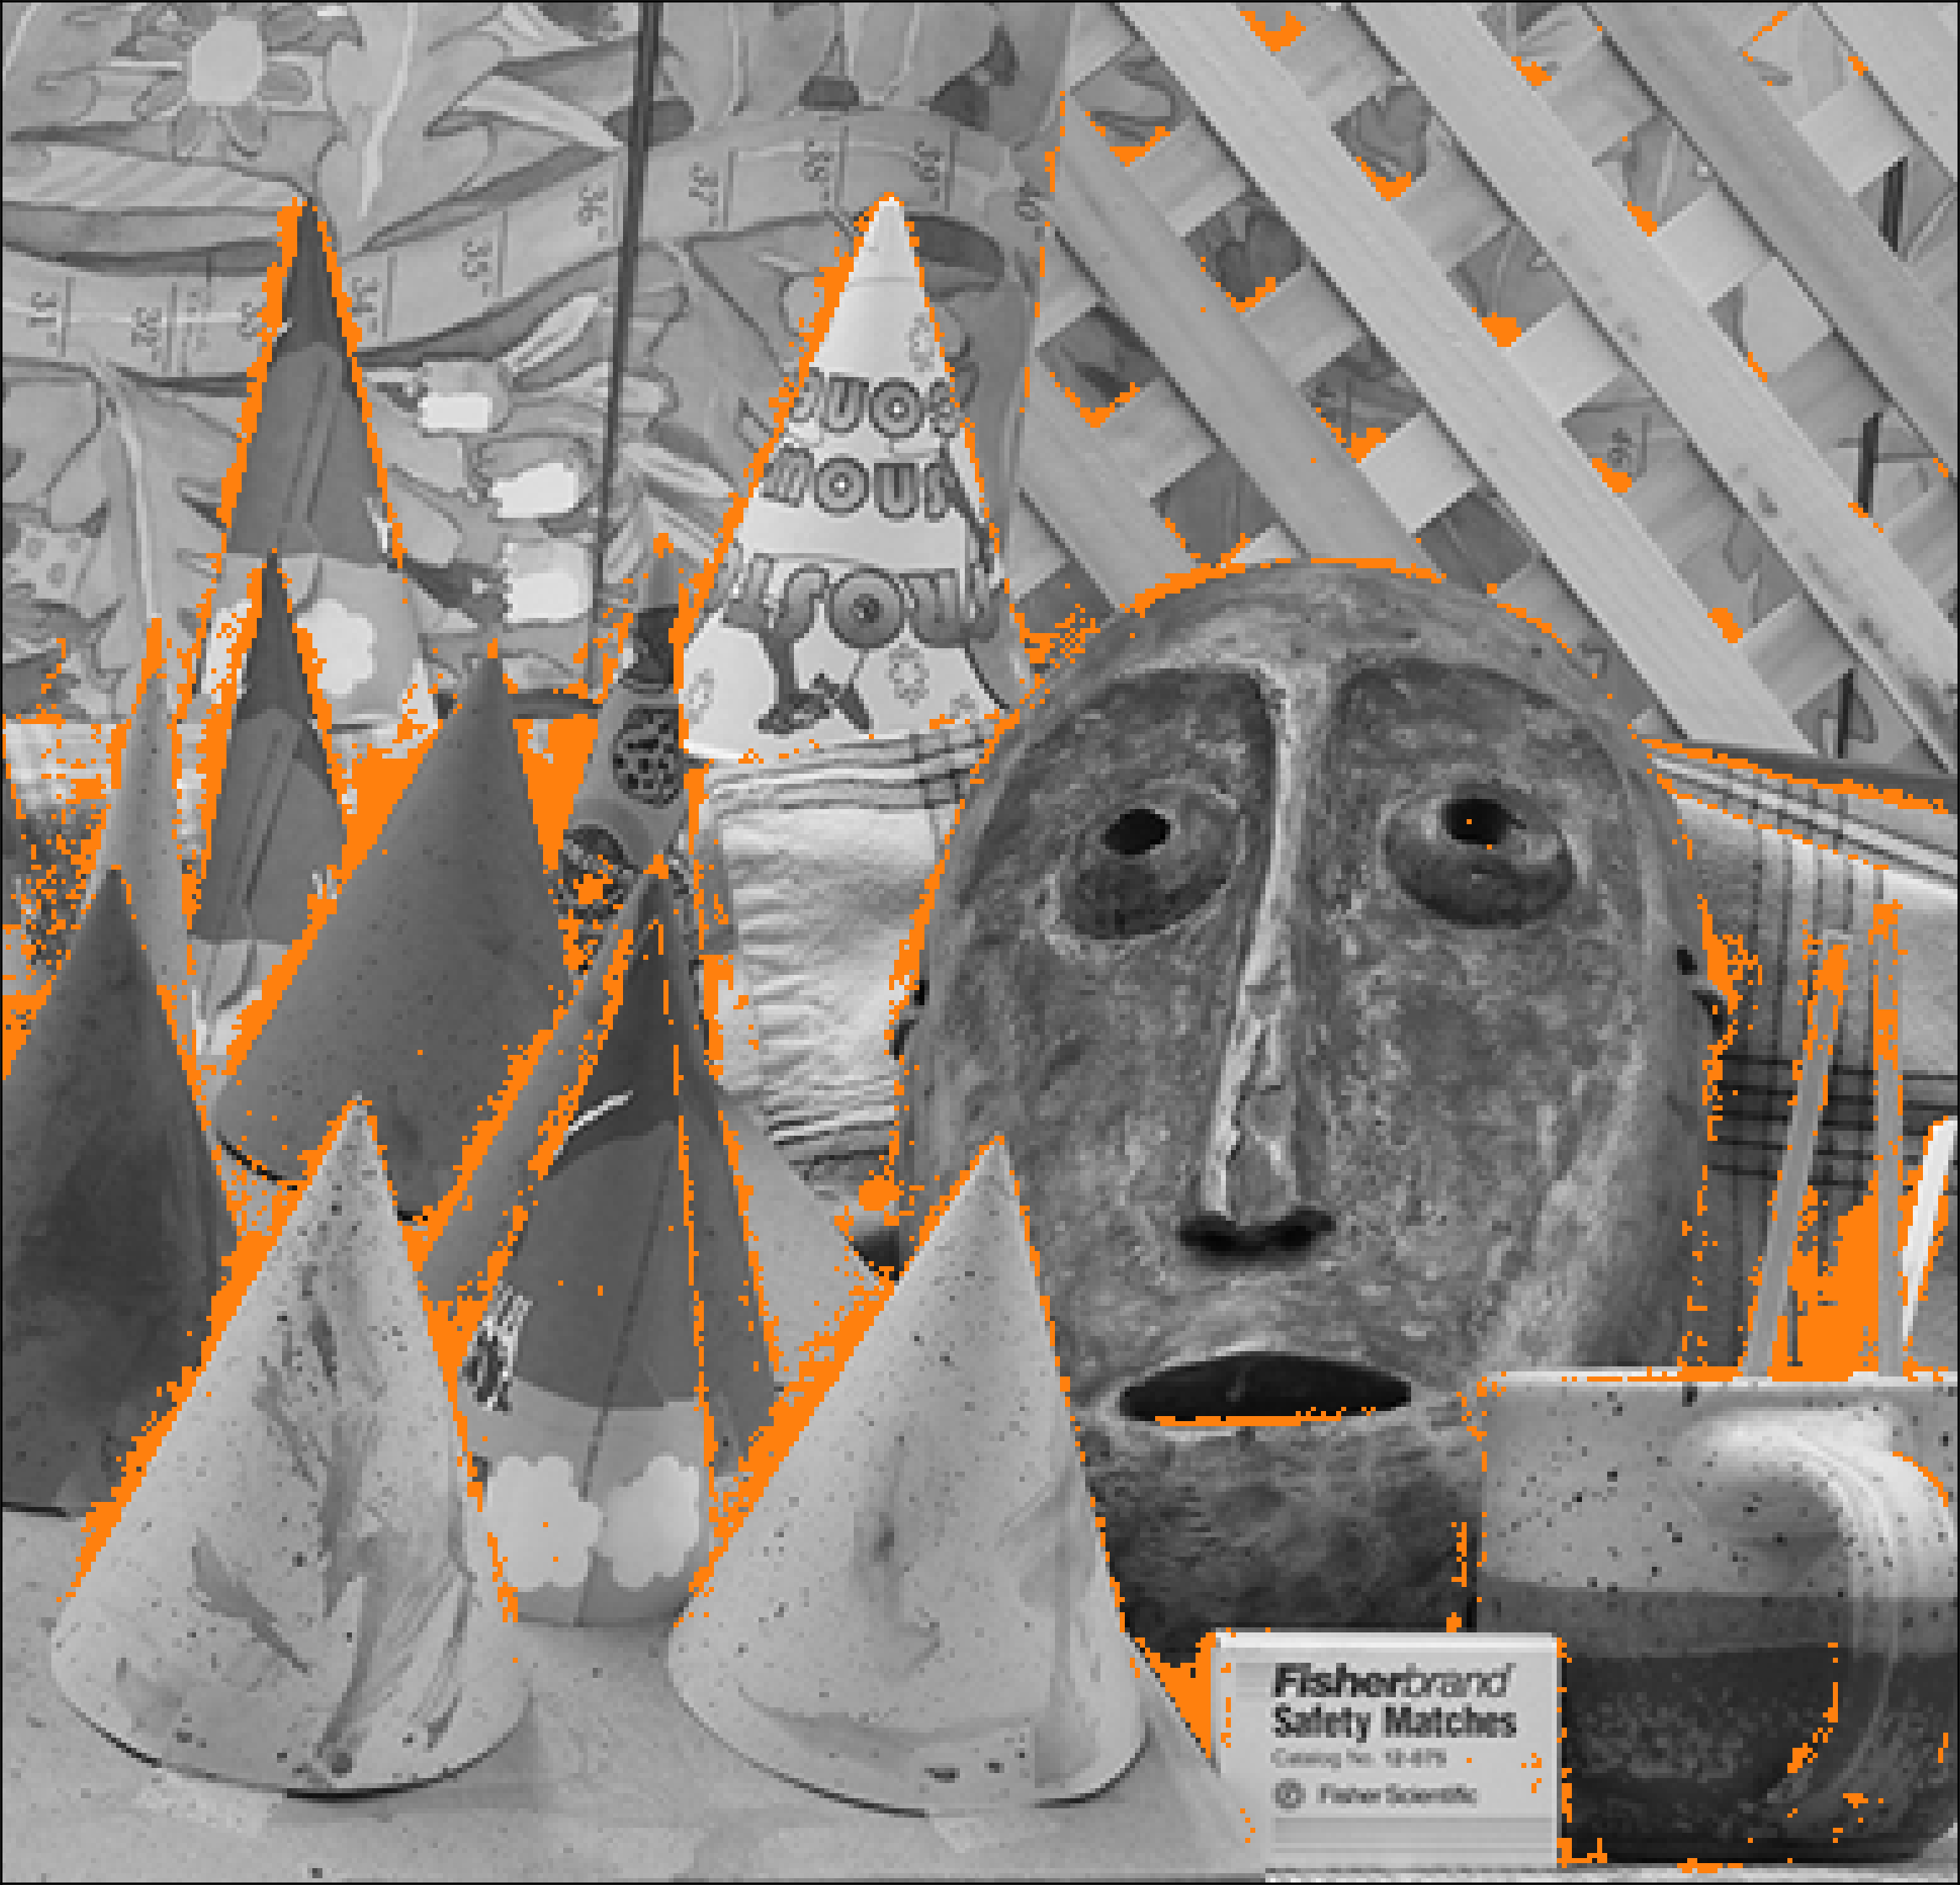
\includegraphics[width=\linewidth]{Images/Chap_5/comparison_wrong_intervals_no_reg.png}
        \caption{Without regularization, filtering and refinement}
        \label{fig:comparison_wrong_intervals_no_reg}
    \end{subfigure}
    \hfill\begin{subfigure}[t]{0.49\linewidth}
        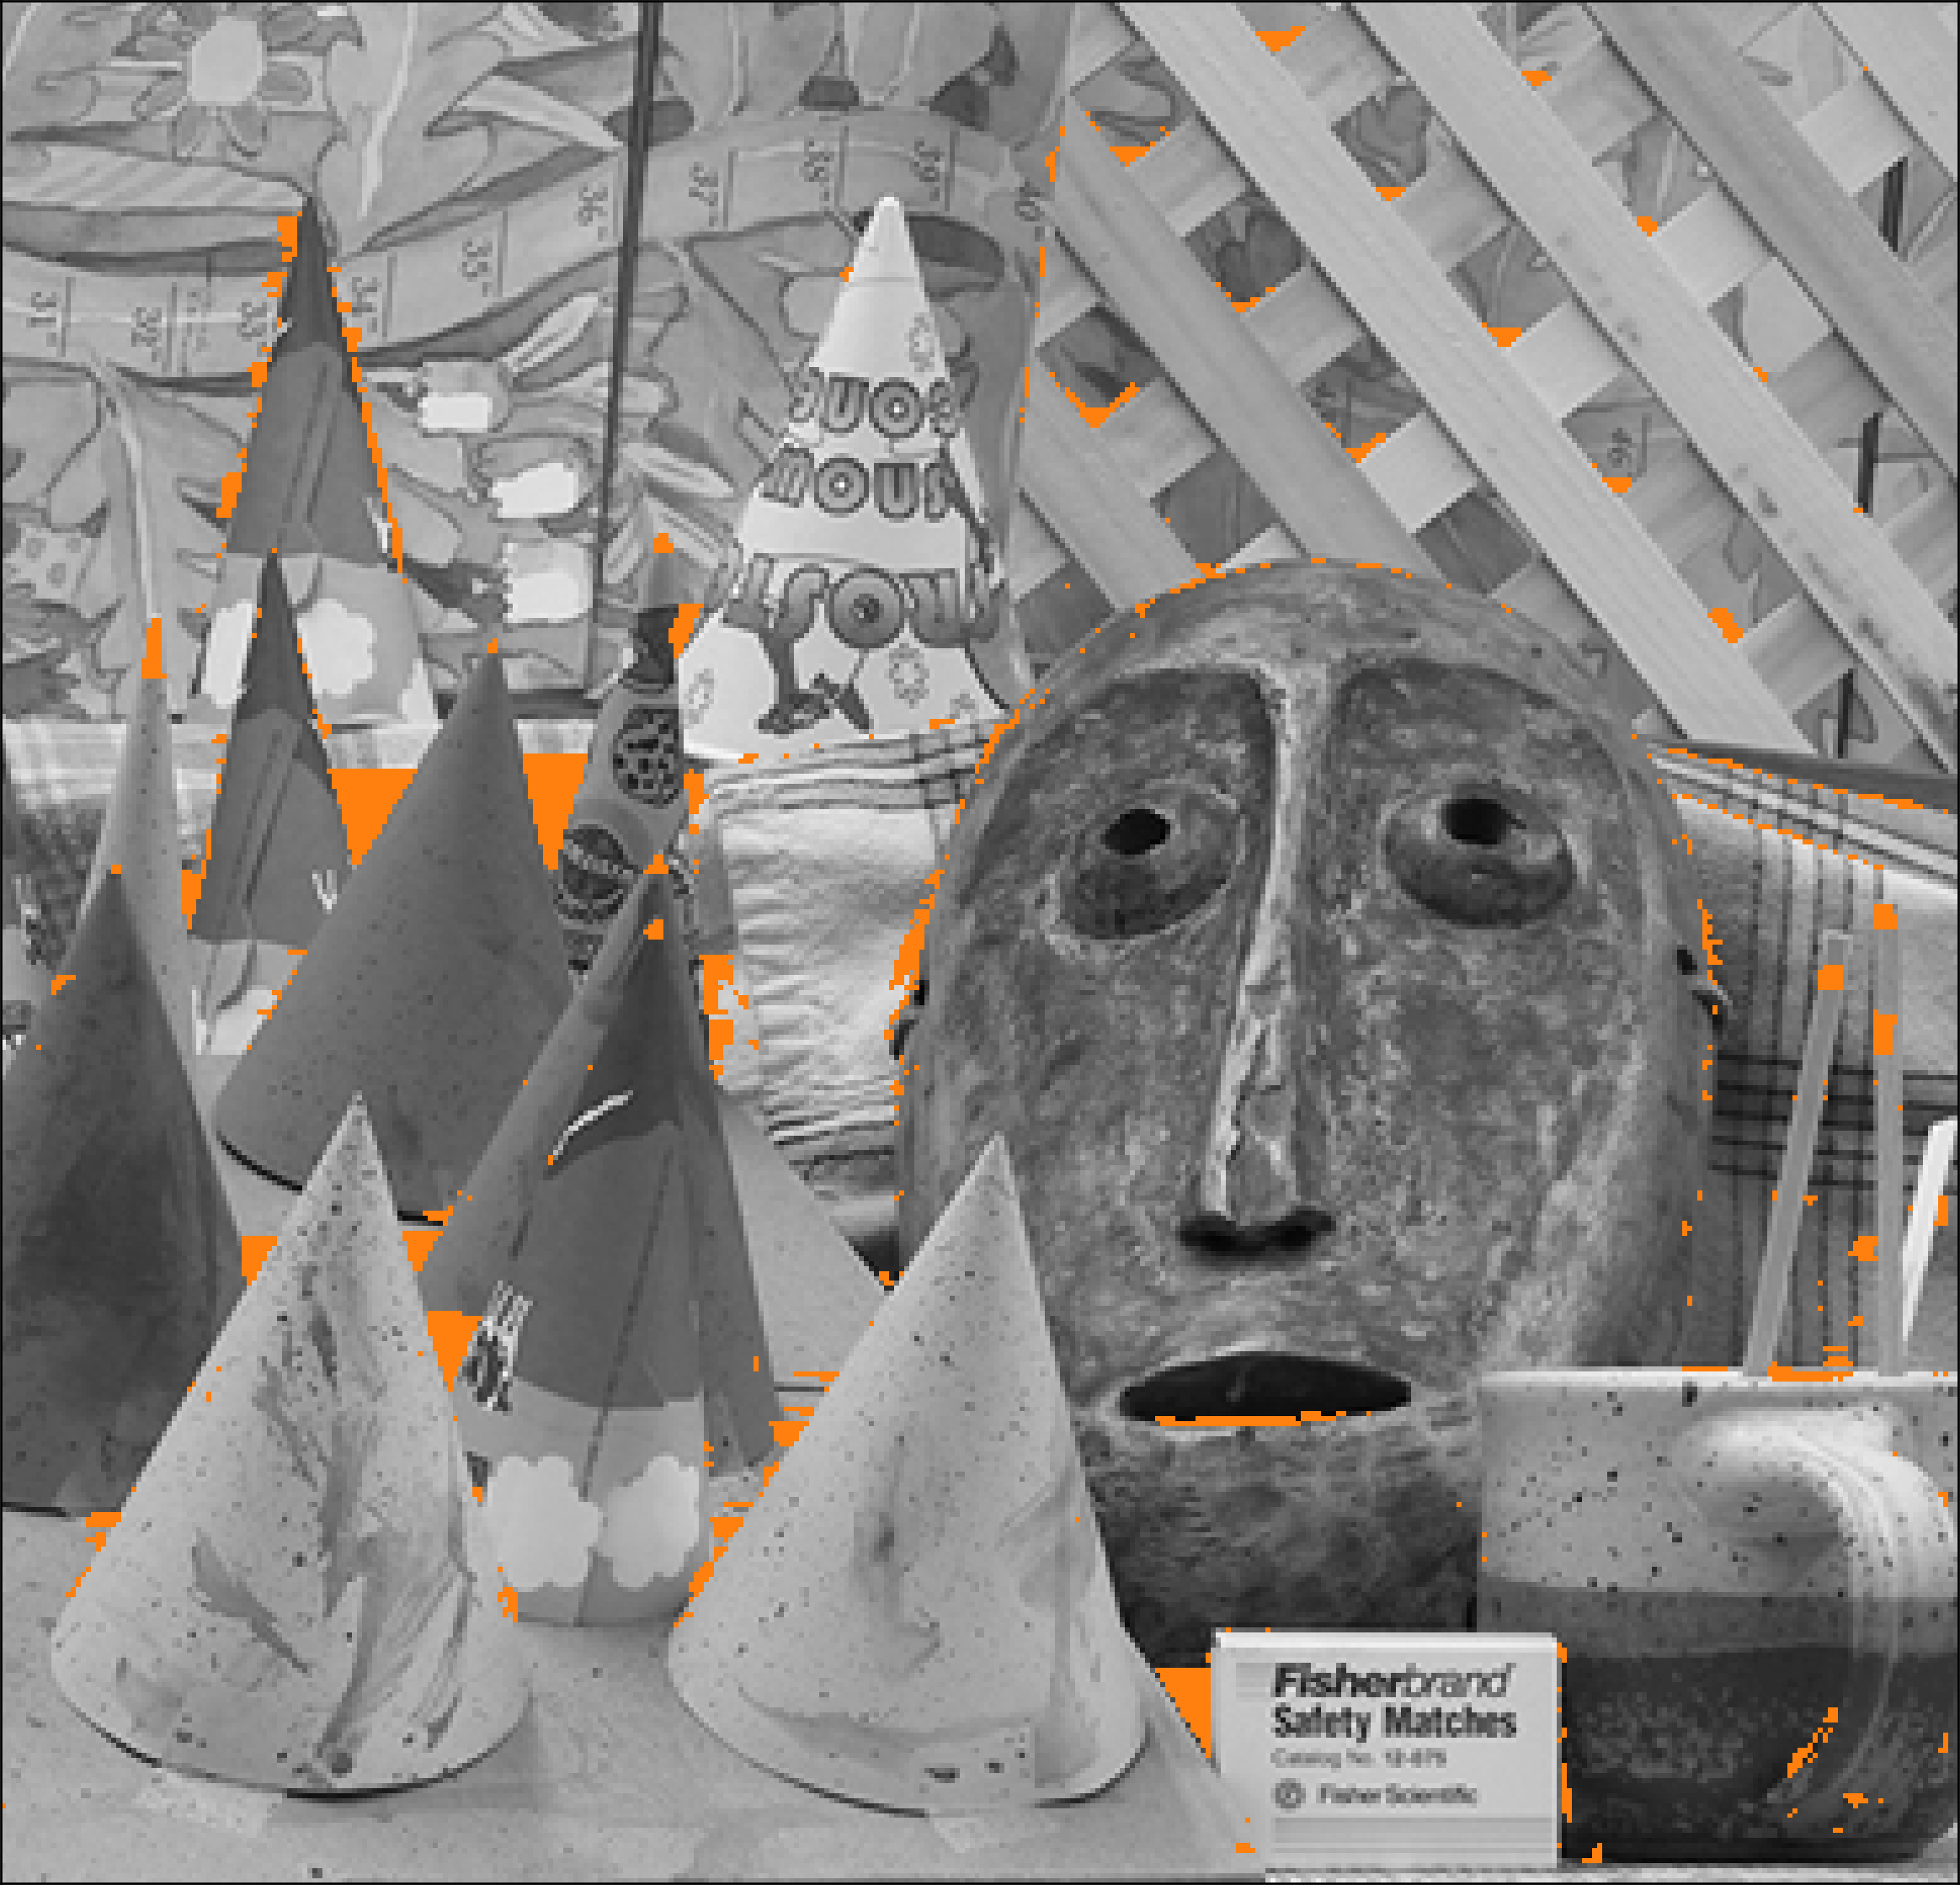
\includegraphics[width=1\linewidth]{Images/Chap_5/comparison_wrong_intervals_reg.png}
        \caption{With regularization, filtering and refinement}
        \label{fig:comparison_wrong_intervals_reg}
    \end{subfigure}
    \caption{Left image from Middlebury cones. Confidence intervals that do not contain the ground truth appear in orange.}
    \label{fig:comparison_wrong_intervals}
\end{figure}

\Cref{fig:comparison_wrong_intervals} allows visualizing the position of wrong intervals in the left stereo image. We can see clear improvements between the method with and without regularization. This can especially be observed in the bottom right corner of images near the sticks inside the cup, or in general near cones borders. Quantitatively, wrong intervals represent around $5\%$ of pixels without regularization, and $1.6\%$ with regularization. Those numbers are presented for information purposes only, as further scores will be computed on different scenes, allowing for more in-depth analysis.

This concludes the method for computing disparity confidence intervals in the dense stereo matching part of the photogrammetry pipeline. We will see next how those intervals can be propagated into confidence intervals for the \acrshort{dsm}s.

\section{Evaluation of Disparity Intervals}
\subsection{Metrics for Evaluating the Accuracy and Size}\label{sec:metrics_disparity}
In order to evaluate the performance of the disparity confidence intervals, we will now introduce some metrics. To the best of our knowledge, there is no current method for producing disparity confidence intervals to use for comparison. The objective of this section is to propose a range of tools able to quantify the trade-off between accuracy and size of intervals. For each metric, we do not consider pixels without ground truth, pixels at the border of images that cannot fully explore their disparity range, or pixels discarded by the cross-checking test (\Cref{eq:cross-checking}). Pixels at the border of an image  for which the disparity range cannot be fully explored were also discarded, as the ground truth exists but is often unreachable. 

\subsubsection{Accuracy}
The first and most obvious metric is the proportion of correct intervals, \ie intervals containing the true disparity, which we call accuracy $acc$:
\begin{align}
    acc = \dfrac{\#\{I_\alpha ~|~ \st ~d_{true}\in I_\alpha\}}{\#\{I_\alpha\}}\label{eq:accuracy}
\end{align}
We want to maximize the accuracy, and fixed ourselves a minimal objective of $90\%$ accuracy for our method.

\subsubsection{Residual Error}
It is also interesting to measure the magnitude of the error. We thus introduce another metric called residual error $\varepsilon$, computed for intervals that do not contain the ground truth and defined as:
\begin{align}
    \varepsilon=\median \left( \dfrac{\min(|d_{true}-\overline{I}_\alpha|, |d_{true}-\underline{I}_\alpha|)}{d_{max}-d_{min}}\right)\label{eq:residual_error}
\end{align}
where $[d_{min}, ~d_{max}]$ is the considered disparity range. Normalization by the disparity range yields a metric that can be compared across datasets with different disparity ranges. For instance, in the 2003 Middlebury ``Cones'' dataset, the disparity range is $[-60, ~0]$, while in the 2014 Middlebury ``Shopvac-perfect'' dataset, the disparity range is $[-1100, ~0]$.

Residual error and other metrics are defined using the $\median$ of a set, instead of the mean, so as to be less sensitive to outliers. We will still present the distributions of the metrics without the median operator in \Cref{sec:results_disparity}. The residual error allows quantifying how ``wrong'' were the intervals. A residual error near $0$ translate the fact that the confidence intervals were really close to capture the ground truth, while a residual error near $1$ indicate that the intervals were far off the ground truth. \Cref{fig:residual_error} helps to visualize $\varepsilon$.

Because half of pixels have a relative error less than $\varepsilon$, extending each bound of the intervals by $\varepsilon\cdot(d_{max}-d_{min})$ effectively divides the global error by two. The accuracy would therefore be $acc'=acc+\dfrac{(1-acc)}{2}$. $\varepsilon$ thus provides a quick and easy estimation of the length missing to the intervals in order to divide the missing accuracy by two.

\subsubsection{Relative Size}
We now introduce a metric to measure the size of intervals. This metric evaluates the relative size of intervals, with regard to the size of the considered disparity range:
\begin{align}\label{eq:relative_size_disparity}
    s_{rel}=\median\left(\dfrac{\overline{I}_\alpha-\underline{I}_\alpha}{d_{max}-d_{min}}\right)
\end{align}
where $[d_{min}, ~d_{max}]$ is the considered disparity range. We use the same normalization as for the residual error $\varepsilon$ We want to minimize $s_{rel}$ to ensure our intervals are not too large.

\subsubsection{Relative Over-Estimation}
During the regularization of confidence intervals, we purposefully extended the bounds of the intervals in low confidence areas. The relative size of intervals $s_{rel}$ in those areas will, by design, be very large. We therefore propose to evaluate the relative size only on high confidence areas, and to introduce a specific measure for low confidence areas, called relative over-estimation. Defined when intervals correctly contain the true disparity, it is computed as follows:
\begin{align}
    o_{rel}=\median\left(1-\dfrac{\Delta|d_{true}-\tilde{d}|}{\overline{I}_\alpha-\underline{I}_\alpha}\right)\label{eq:relative_overestimation_disparity}
\end{align}
where $\Delta|d_{true}-\tilde{d}|$ is defined as:
\begin{align}
    \Delta|d_{true}-\tilde{d}|=\max(\{&|d_{true}(row', ~col')-\tilde{d}(row'', ~col'')|, \text{ with}~\nonumber\\&(row',~col')\in \N(\rowcol), ~ (row'',~col'')\in \S(\rowcol)\})
\end{align}
In other words, $\Delta|d_{true}-\tilde{d}|$ is the maximal difference between the true disparity and the predicted disparity over the same low confidence segment. We consider $S(\rowcol)$ and not the whole neighboring $\N(\rowcol)$ as the intervals have the same value only in a segment $S$ (see \Cref{sec:regularization_of_intervals} for more details). Note that the true disparity and predicted disparity can belong to two different pixels in the computation of $\Delta|d_{true}-\tilde{d}|$. $\Delta|d_{true}-\tilde{d}|$ is the size of the optimal interval, \ie the smallest interval containing both $d_{true}$ and $\tilde{d}$ in the low confidence area. $1-\dfrac{\Delta|d_{true}-\tilde{d}|}{\overline{I}_\alpha-\underline{I}_\alpha}$ therefore represent the superfluous proportion of intervals, or in other words, the proportion of $\overline{I}_\alpha-\underline{I}_\alpha$ that is over-estimating the error $\Delta|d_{true}-\tilde{d}|$. \Cref{fig:relative_overestimation} illustrates the meaning of $\Delta|d_{true}-\tilde{d}|$ and $I_\alpha$ for the computation of the relative over-estimation inside a low confidence area.

Because we want to obtain the smallest possible correct intervals, it only makes sense to compute $o_{rel}$ for confidence intervals that do contain the true disparity. Indeed, considering wrong intervals could reduce the over-estimation and induce bias in our conclusions. Doing so also insure $o_{rel}$ is always contained between $0$ and $1$, and can be expressed as a percentage.

We want the relative over-estimation to be as close to $0$ as possible, as $o_{rel}=0$ means that $I_\alpha$ is the optimal interval for at least half of the low confidence pixels. $1-\dfrac{\Delta|d_{true}-\tilde{d}|}{\overline{I}_\alpha-\underline{I}_\alpha}=0.1$ means that the superfluous part of the interval represents a tenth of its total length. Similarly, $1-\dfrac{\Delta|d_{true}-\tilde{d}|}{\overline{I}_\alpha-\underline{I}_\alpha}=0.5$ means that the superfluous part of the interval represents half of their total length.

Reaching a relative over-estimation of $0$ is not realistic, as it would be equivalent to say that we exactly know the position of the true disparity for each pixel. This is irrational, as it would mean we have the perfect stereo matching algorithm, but somehow still predicted a wrong disparity. A more realistic objective is to be around $50\%$, even though less is better.

\begin{figure}
    \centering
    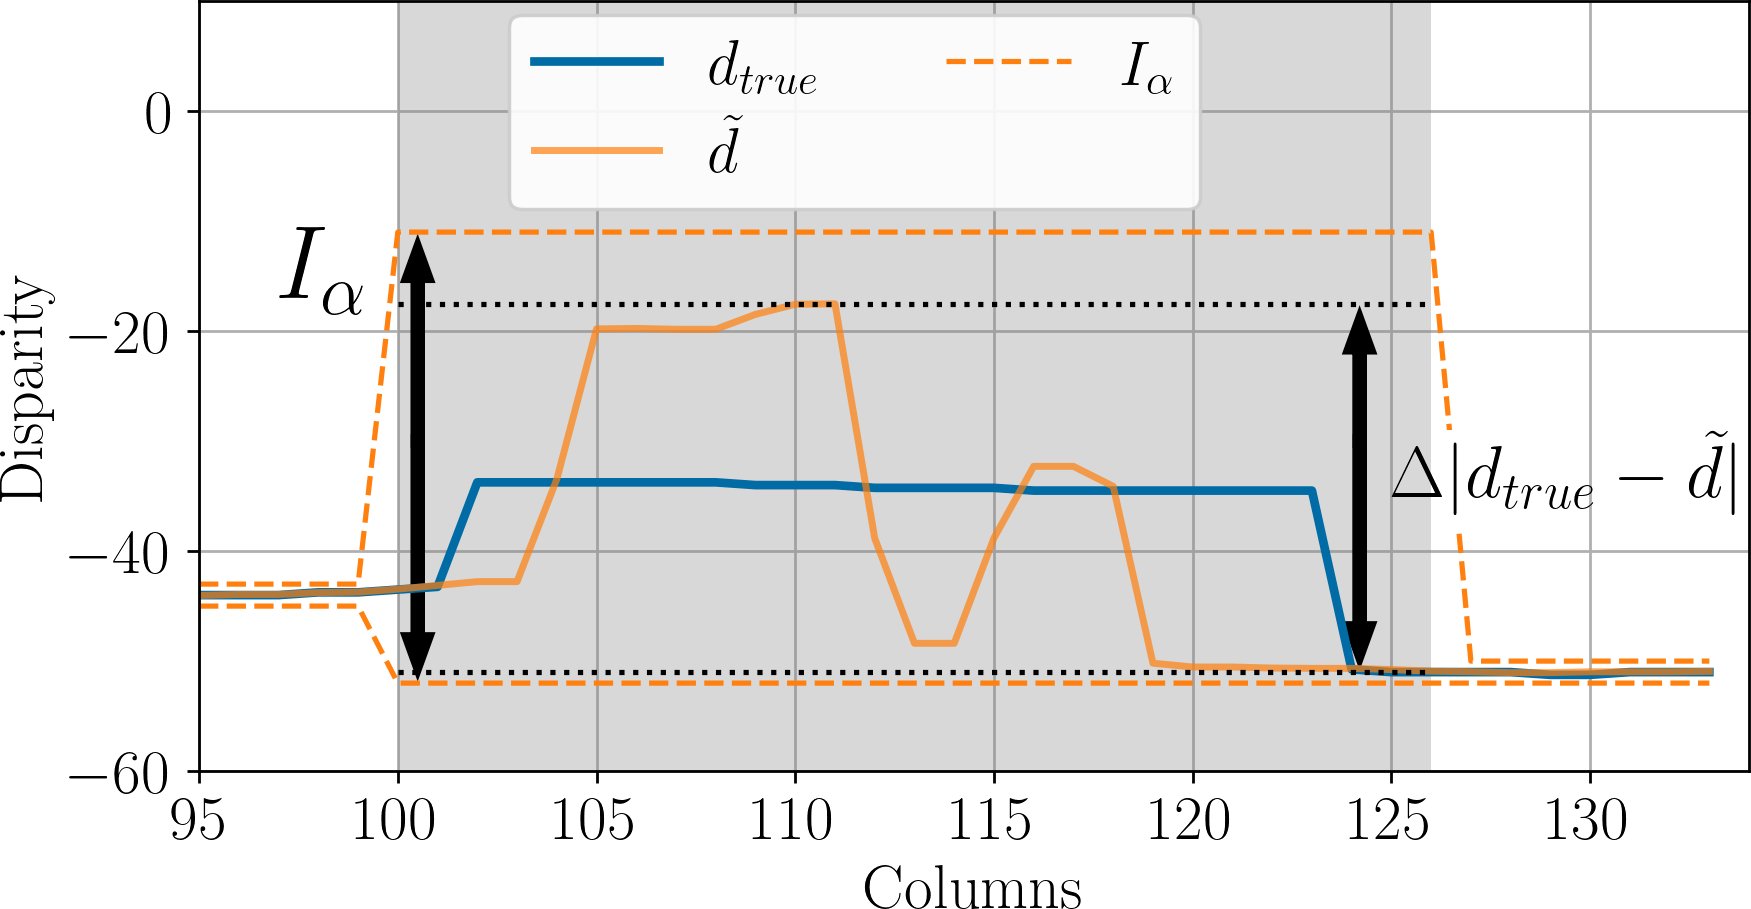
\includegraphics[width=0.8\linewidth]{Images/Chap_5/relative_overestimation_row_230.png}
    \caption{$\Delta|d_{true}-\tilde{d}|$ and $I_\alpha$ for computing the relative estimation (\Cref{eq:relative_overestimation_disparity}) over a low confidence area in gray.}
    \label{fig:relative_overestimation}
\end{figure}

\begin{figure}
    \centering
    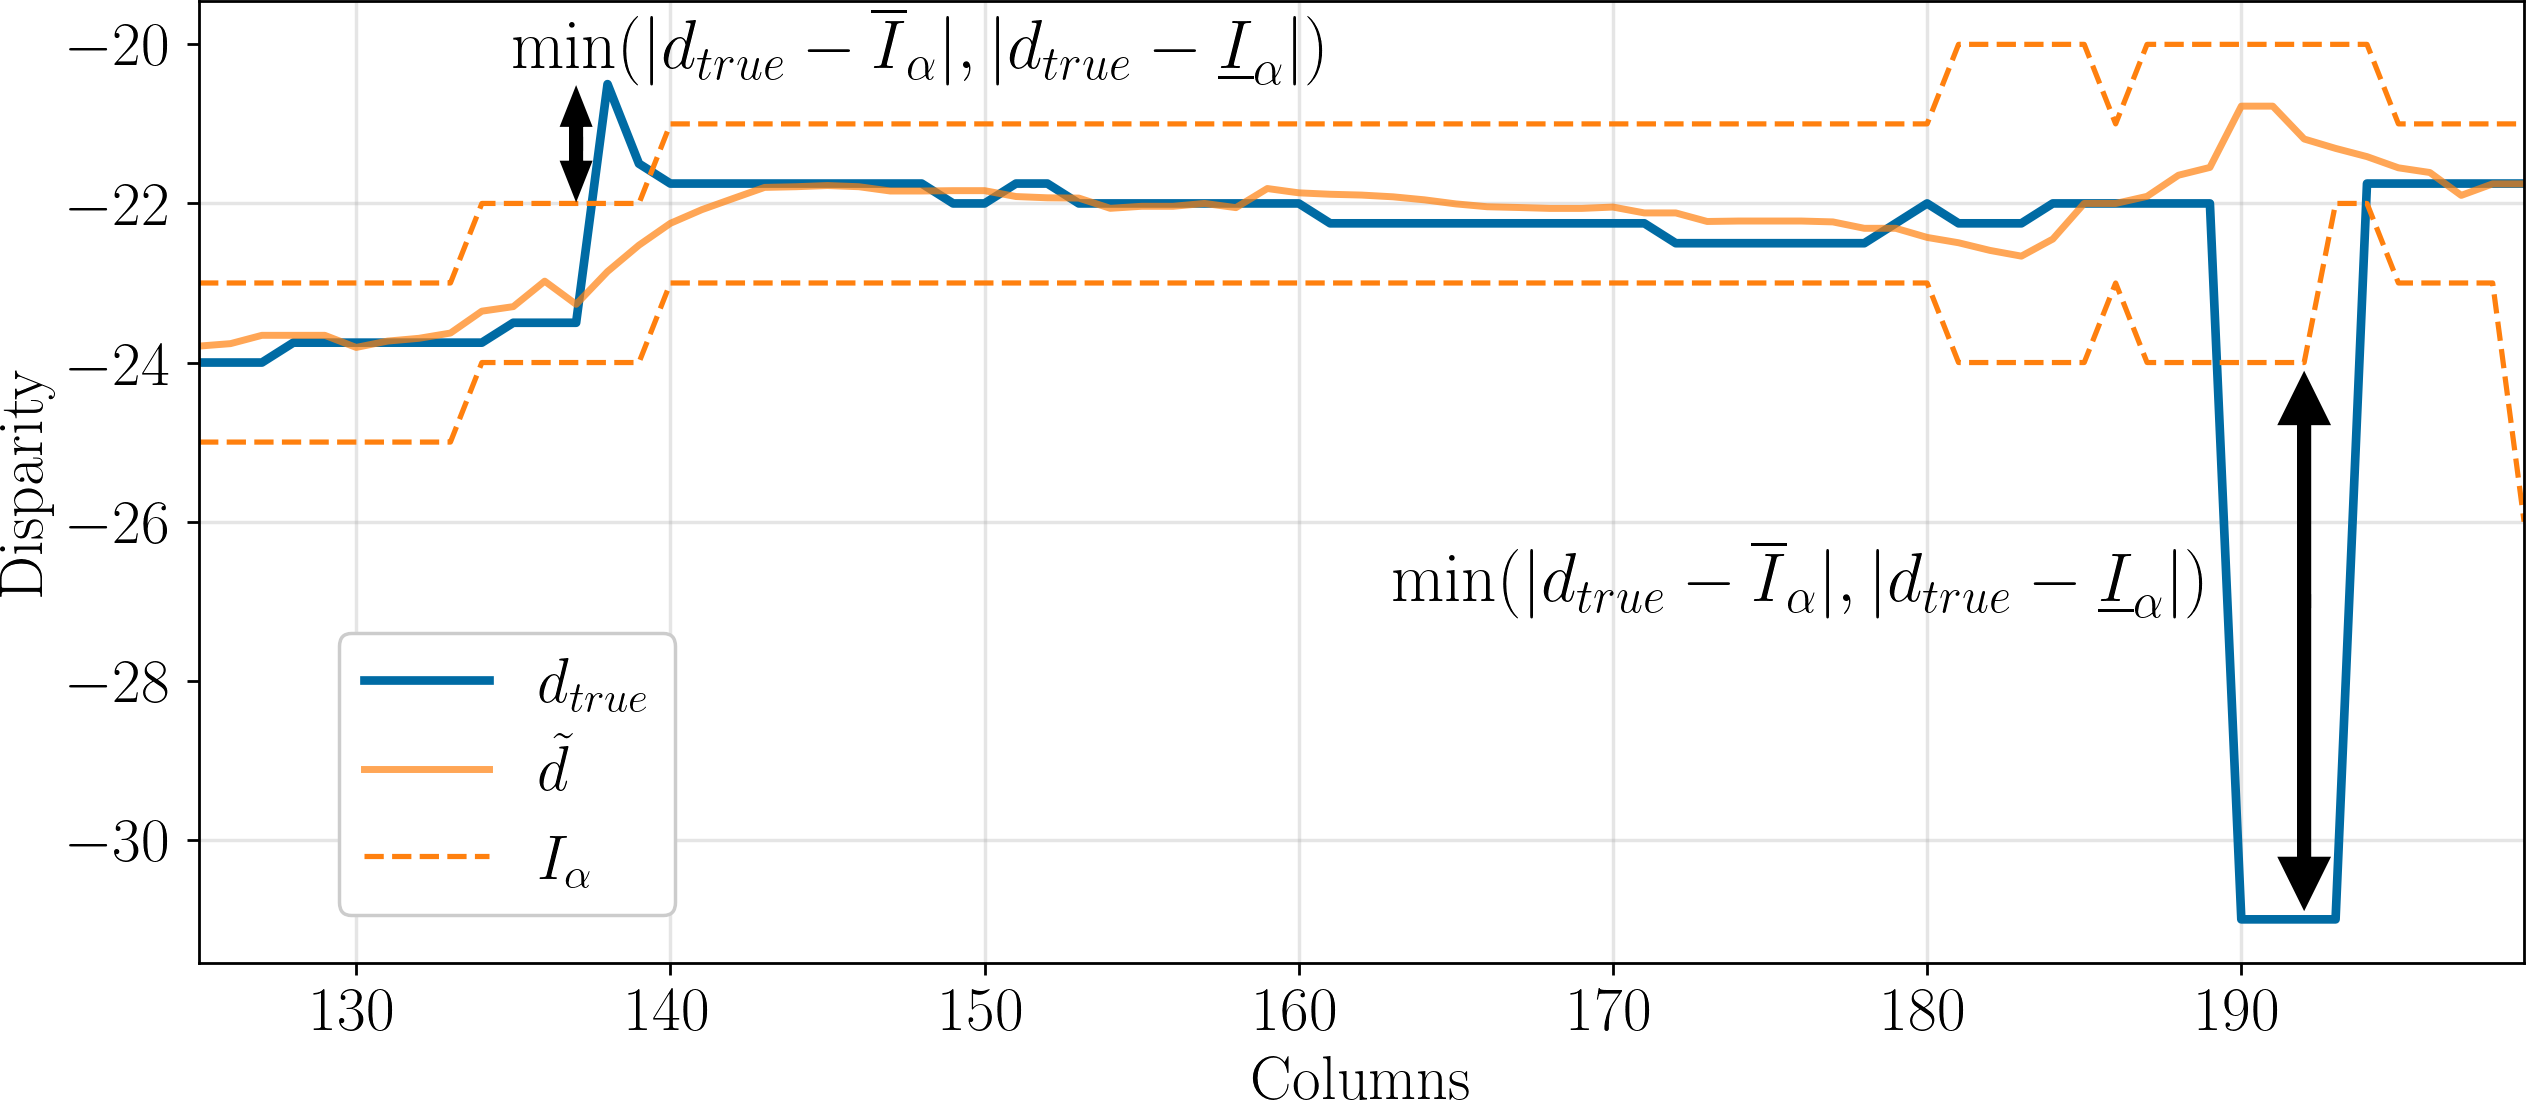
\includegraphics[width=0.8\linewidth]{Images/Chap_5/residual_error_row_108.png}
    \caption{Different values of $\min(|d_{true}-\overline{I}_\alpha|, |d_{true}-\underline{I}_\alpha|)$ for computing the residual error of \Cref{eq:residual_error}}
    \label{fig:residual_error}
\end{figure}

\begin{remark}
    The relative over-estimation could theoretically reach a value of $1$ regardless of the size of intervals if $\Delta|d_{true}-\tilde{d}=0$. This is the case if and only if the predicted disparity and the true disparity are equal and constant for all pixels in the considered low confidence area. This is however very unlikely, as low confidence areas are usually areas with strong variations of disparity, and where the stereo algorithm struggles to predict a correct disparity.
\end{remark}

Because we evaluate the size of intervals using two different metrics depending on if intervals are in low confidence areas or not, it is interesting to measure the proportion of low confidence areas in the scene $p_{amb}$:
\begin{align}
    p_{amb} = \dfrac{\#\{I_\alpha ~|~I_\alpha\in\mathrm{low~confidence~area}\}}{\#\{I_\alpha\}}
\end{align}
A proportion $p_{amb}$ of intervals size will be evaluated using $o_{rel}$, and a proportion $1-p_{amb}$ using $s_{rel}$. A high $p_{amb}$ thus indicates many regularizations and consequently larger intervals in general.

Before measuring the accuracy of intervals using $acc$, to quantify their errors using $\varepsilon$ or measuring their relative size with $s_{rel}$ and $o_{rel}$, we will present the different considered datasets used for our evaluation.

\subsection{Stereo Matching Dataset}\label{sec:dataset}
We evaluate the disparity confidence intervals on $76$ scenes from the Middlebury datasets. Those datasets are composed of two stereo images of indoor scenes, for which the true disparity is exactly known. It is divided in different years: 2003, 2005, 2006, 2014, and 2021 \cite{scharstein_high-accuracy_2003, scharstein_learning_2007, hirschmuller_evaluation_2007, scharstein_high-resolution_2014}, and the complexity of scenes increases with years. \Cref{fig:middlebury_examples} present some scenes from each dataset. Each dataset is available in different resolutions. We use quarter-size and third-size versions of the data for 2003, 2005 and 2006 datasets and full resolution for 2014 and 2021 datasets in order to include a diversity of resolutions in our experiments. As a result, ranges of considered disparities also vary greatly. For instance, disparity ranges of the 2014 dataset are very large (more than a thousand disparity wide), which presents a significant challenge for the stereo matching algorithm, as many disparities need to be explored. On those scenes, our stereo matching algorithm performs far less well than on the 2003 dataset. This allows evaluating whether the disparity confidence intervals can perform well even when the main disparity predictions do not. Each dataset does not contain the same number of images, and shapes of images can vary across datasets and inside each dataset. For indication purposes, datasets from 2003, 2005, 2006, 2014, and 2021 respectively contain 2, 6, 21, 23 and 25 scenes.

\begin{figure}
    \centering
    \begin{subfigure}[t]{0.33\linewidth}
        \centering
        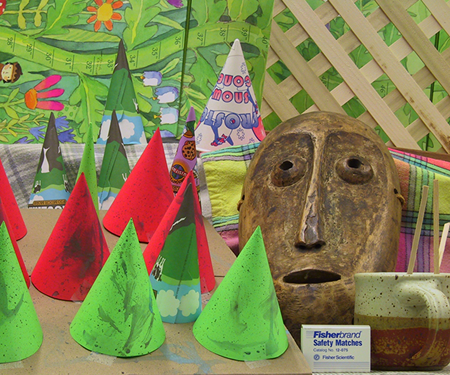
\includegraphics[width=\linewidth]{Images/Chap_5/2003cones.png}
        \caption{2003 Cones}
        \label{fig:2003_cones}
    \end{subfigure}\hfill
    \begin{subfigure}[t]{0.33\linewidth}
        \centering
        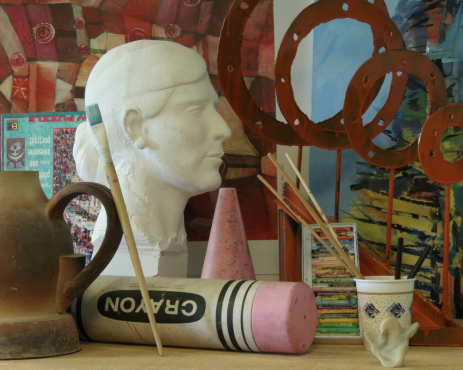
\includegraphics[width=\linewidth]{Images/Chap_5/2005art.png}
        \caption{2005 Art}
        \label{fig:2005_art}
    \end{subfigure}\hfill
    \begin{subfigure}[t]{0.33\linewidth}
        \centering
        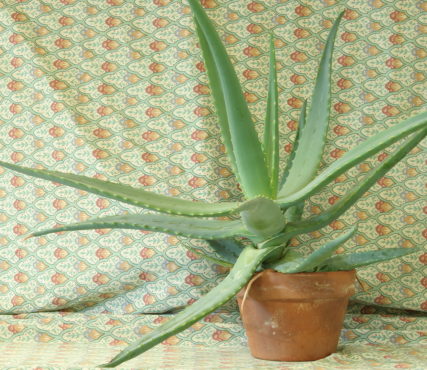
\includegraphics[width=\linewidth]{Images/Chap_5/2006aloe.png}
        \caption{2006 Aloe}
        \label{fig:2006_aloe}
    \end{subfigure}\hfill
    \begin{subfigure}[t]{0.33\linewidth}
        \centering
        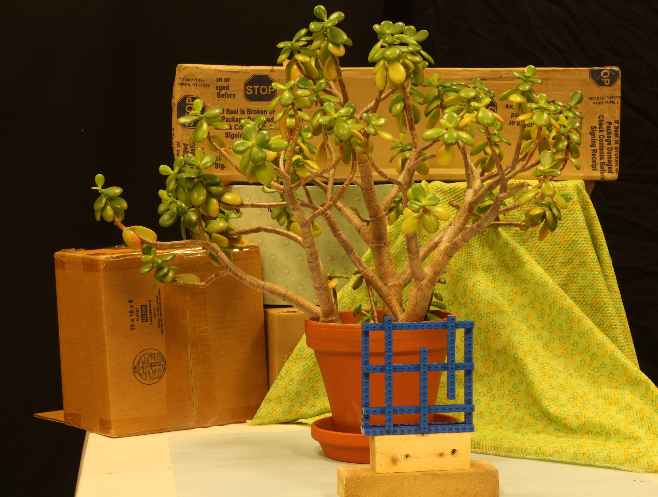
\includegraphics[width=\linewidth]{Images/Chap_5/2014_Jadeplant-perfect.png}
        \caption{2014 Jadeplant Perfect}
        \label{fig:2014_jadeplant}
    \end{subfigure}\hfill
    \begin{subfigure}[t]{0.33\linewidth}
        \centering
        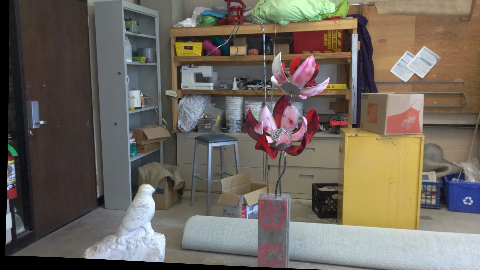
\includegraphics[width=\linewidth]{Images/Chap_5/2021_artroom1.png}
        \caption{2021 Artroom1}
        \label{fig:2021_artroom1}
    \end{subfigure}\hfill
    \begin{subfigure}[t]{0.33\linewidth}
        \centering
        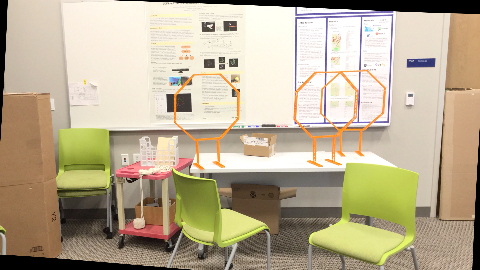
\includegraphics[width=\linewidth]{Images/Chap_5/2021_octogons1.png}
        \caption{2021 Octogons1}
        \label{fig:2021_octogons1}
    \end{subfigure}
    \caption{Example of left images from  different Middlebury datasets}
    \label{fig:middlebury_examples}
\end{figure}

The Middlebury dataset contains generic indoor scenes with a high variety of 3D structures, which highlights the potential of our method for any stereo algorithm. Our objective is however to process satellite images, so we also evaluate our method on satellite data, which can greatly differ from indoor scenes. For this purpose, we use 80 pairs of $1845\times1845$ satellite images in epipolar geometry, with a typical disparity range of $[-20, 10]$ (it slightly varies between images). Those images are all part of the same pair of Pléiades images over the city of Montpellier (France), which is large enough to contain both urban and rural areas, as presented in \Cref{fig:mtp_img}. The ground truth of those images was obtained using the method described in \cite{cournet_ground_2020}. In a few words, this method first processes stereo images to obtain images in epipolar geometry. Then it considers the ground truth \acrshort{dsm} of the scene, for instance a rasterized \acrshort{lidar} HD data, and project it into the same geometry as one of the sensors. Then, using the disparity to altitude ratio computed alongside epipolar images, it converts the altitude of the re-projected ground truth \acrshort{dsm} into disparities. Using the same epipolar grids, this true disparity map can be projected into epipolar geometry. We now have two stereo images and their associated ``ground truth'' disparity map in epipolar geometry, ready to be processed. This method has a few known drawbacks. First, the ground truth is resampled in two different geometries, which relies on the quality of the epipolar grid, the planimetric accuracy of the ground truth data, and satellite images. Secondly, the images and ground truth were acquired a few years apart, which results in some new buildings being built or destroyed between stereo images and ground truth. The vegetation also changed, so the ground truth is not always $100\%$ correct. The dataset initially contained 327 pairs of images, but we detected major differences between the ground truth and the epipolar images, as illustrated in \Cref{fig:mtp_278}, so we restricted our selection to 80 pairs that did not exhibit major differences. The evaluation metrics on this dataset must thus be taken with care.

\begin{figure}[ht!]
    \centering
    \begin{subfigure}[t]{0.4\linewidth}
        \centering
        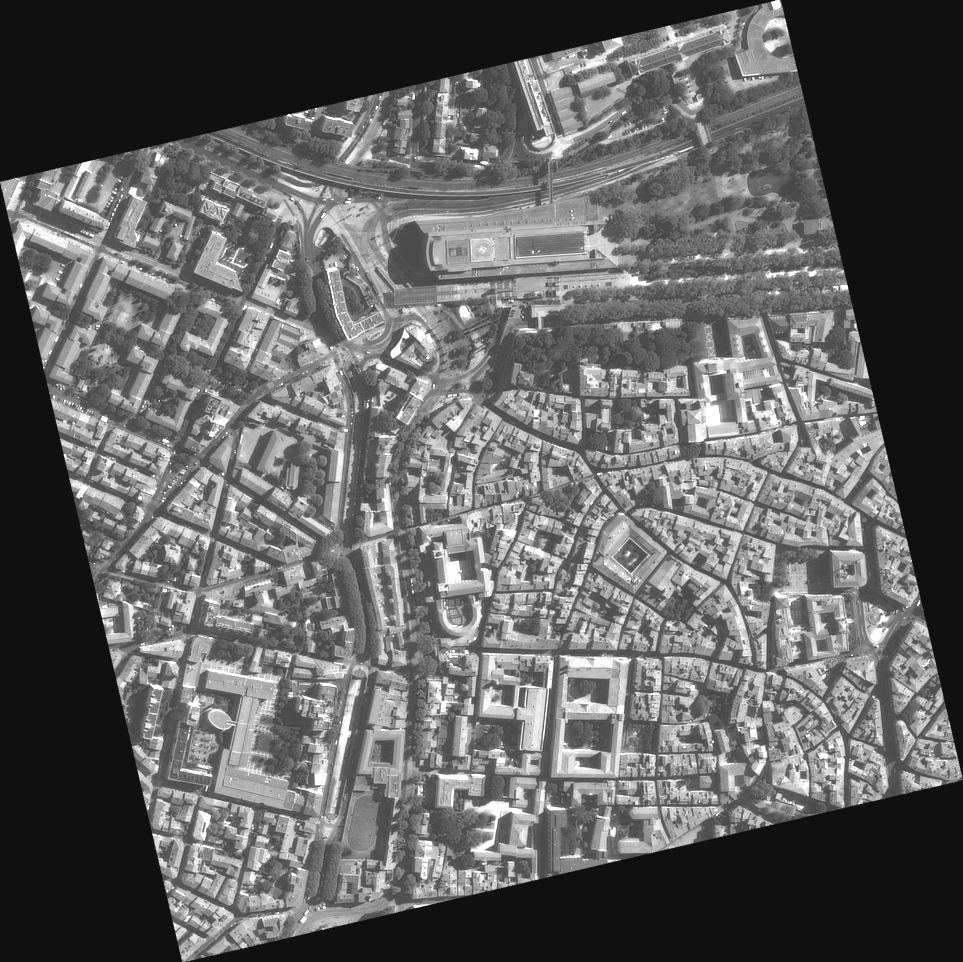
\includegraphics[width=\linewidth]{Images/Chap_5/img_MTP_120.png}
        \caption{Left epipolar image}
        \label{fig:mtp_img_a}
    \end{subfigure}\hfill
    \begin{subfigure}[t]{0.4\linewidth}
        \centering
        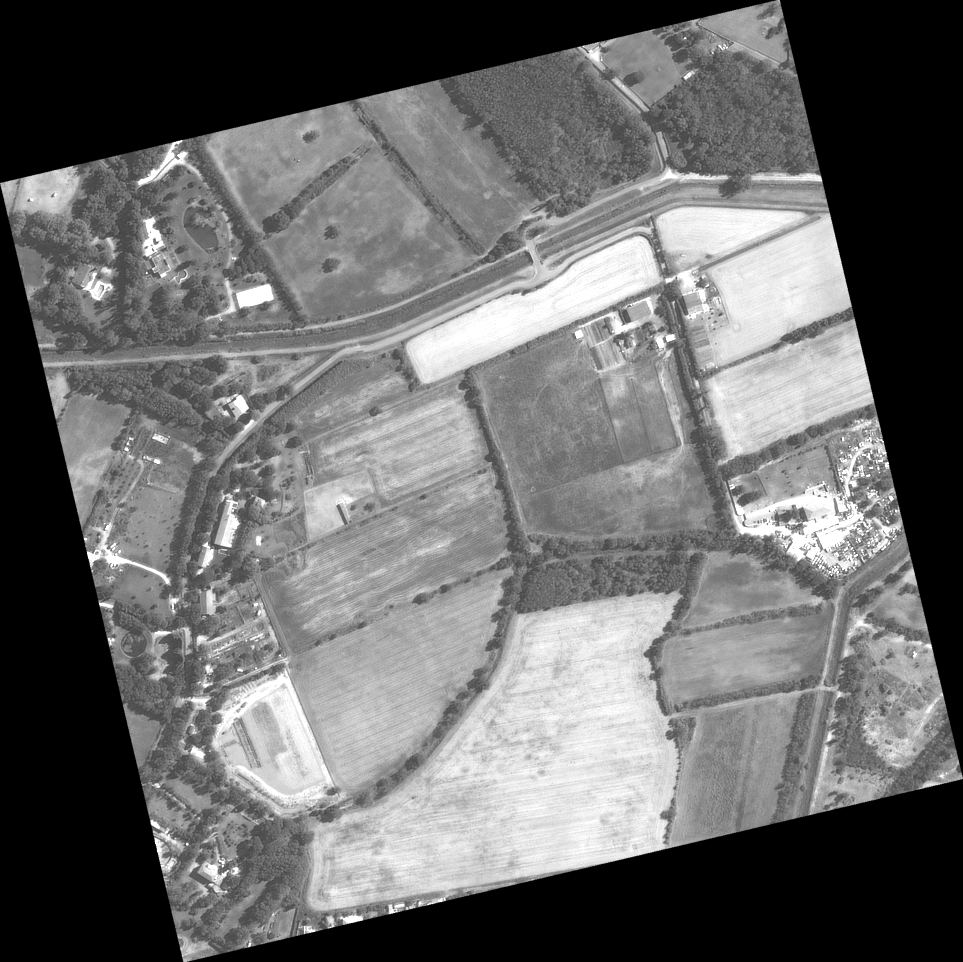
\includegraphics[width=\linewidth]{Images/Chap_5/img_MTP_153.png}
        \caption{Left epipolar image}
        \label{fig:mtp_img_b}
    \end{subfigure}\\
    \begin{subfigure}[t]{0.4\linewidth}
        \centering
        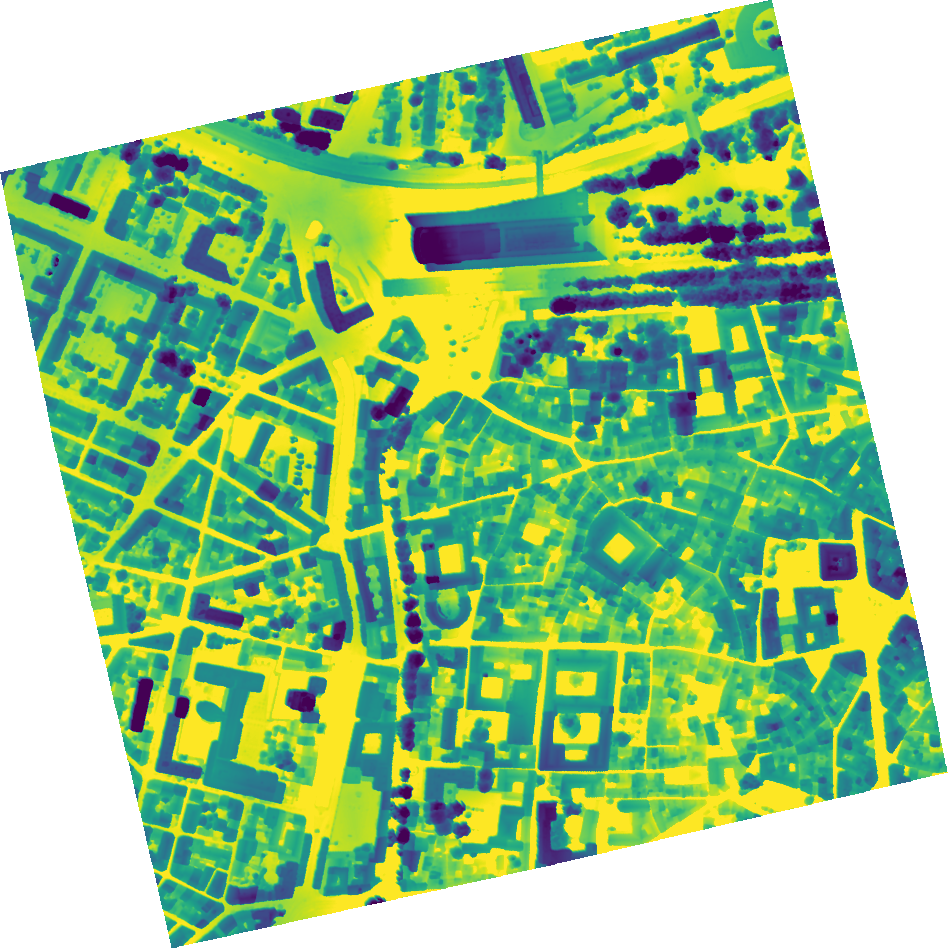
\includegraphics[width=\linewidth]{Images/Chap_5/img_MTP_120_gt.png}
        \caption{Ground truth disparity}
        \label{fig:mtp_img_c}
    \end{subfigure}\hfill
    \begin{subfigure}[t]{0.4\linewidth}
        \centering
        \includegraphics[width=\linewidth]{Images/Chap_5/img_MTP_153_gt.png}
        \caption{Ground truth disparity}
        \label{fig:mtp_img_d}
    \end{subfigure}
    \caption{One rural and one urban scene from the Montpellier dataset.} 
    \label{fig:mtp_img}
\end{figure}


\begin{figure}[ht!]
    \centering
    \begin{subfigure}[t]{0.4\linewidth}
        \centering
        \includegraphics[width=\linewidth]{Images/Chap_5/img_error_MTP_278.png}
        \caption{Left epipolar image}
        \label{fig:mtp_278_a}
    \end{subfigure}\hfill
    \begin{subfigure}[t]{0.4\linewidth}
        \centering
        \includegraphics[width=\linewidth]{Images/Chap_5/img_error_MTP_278_err.png}
        \caption{Wrong intervals (red)}
        \label{fig:mtp_278_b}
    \end{subfigure}\\
    \begin{subfigure}[t]{0.4\linewidth}
        \centering
        \includegraphics[width=\linewidth]{Images/Chap_5/img_error_MTP_278_disp.png}
        \caption{Predicted disparity}
        \label{fig:mtp_278_c}
    \end{subfigure}\hfill
    \begin{subfigure}[t]{0.4\linewidth}
        \centering
        \includegraphics[width=\linewidth]{Images/Chap_5/img_error_MTP_278_gt.png}
        \caption{Ground truth disparity}
        \label{fig:mtp_278_d}
    \end{subfigure}
    \caption{Important differences between the ground truth and epipolar images. We can see that the road appearing in the left image from \Cref{fig:mtp_278_a} does not appear in the ground truth in \Cref{fig:mtp_278_d}, which results in false negative on the intervals from \Cref{fig:mtp_278_b}. The road must have been constructed in between the ground truth acquisition and image acquisition. Images with such differences were removed from the Montpellier dataset.} 
    \label{fig:mtp_278}
\end{figure}

In the next section, we will use the Middlebury datasets to evaluate our method on general indoor scenes, and images of Montpellier (abbreviated as $\mathrm{MTP}$) to determine if we can generalize our results to satellite imagery. We will also consider two cost functions: the CENSUS cost function and MC-CNN cost function, both detailed in \Cref{sec:cost_volume_computation}.

We also remind here the configuration of the stereo matching algorithm used. The CENSUS cost function uses a $5\times5$ window, and \acrshort{sgm} penalties $P_1=8$, $P_2=32$. The MC-CNN cost function uses a $11\times11$ window, and \acrshort{sgm} penalties $P_1=2.3$, $P_2=42.3$. The disparity refinement step uses V-fit interpolation. We also a $3\times3$ median filter on the disparity map. 

\subsection{Results}\label{sec:results_disparity}
This section will evaluate each metric on the different datasets, and for the two considered cost functions, CENSUS and MC-CNN. Because there are a few metrics and many scenes, we first give global results, and gradually go into more details across tables and figures. We first consider global results on Middlebury datasets, as they possess a ground truth of better quality. Each metric is evaluated and averaged over the whole dataset in \Cref{tab:metric_average} to get an overall estimation of its performance. To have a more detailed estimation of scores distribution across scenes, we then plot histograms of each metric across all datasets in \Cref{fig:acc_hist,fig:s_rel_hist,fig:o_rel_hist,fig:eps_hist}. Finally, we will also discuss the metrics by looking at some details of particular scenes in \Cref{fig:piano,fig:mtp_291,fig:sword2}. \Cref{eq:distribution_metrics_cones} also presents the distribution from which some metrics are computed over the Middlebury Cones stereo images.

\begin{table}[ht!]
\centering
\renewcommand{\arraystretch}{1.5}
\begin{tabular}{|c|c||c|c|c|c|c|}
\cline{2-7}
\rowcolor{lightgray}
\multicolumn{1}{c|}{\cellcolor{white}}& Year & 2003 & 2005 & 2006 & 2014 & 2021 \\ \hline

\rowcolor{color_census}
\cellcolor{white} & CENSUS & $97.6\%$ & $96.4\%$ & $99.1\%$ & $94.8\%$ & $91.6\%$\\\cline{2-7}

\rowcolor{color_mccnn}
\multirow{-2}{*}{\cellcolor{white} $acc$ $\uparrow$} & MC-CNN & $97.0\%$ & $97.5\%$ & $99.3\%$ & $98.5\%$ & $99.1\%$\\

\rowcolor{color_census}\hline
\cellcolor{white} & CENSUS & $2.5\%$ & $3.1\%$ & $5.3\%$ & $0.2\%$ & $0.9\%$\\\cline{3-7} 

\rowcolor{color_mccnn}
\multirow{-2}{*}{\cellcolor{white} $\varepsilon_{~~~}$ $\downarrow$} & MC-CNN & $4.0\%$ & $5.6\%$ & $10.0\%$ & $3.8\%$ & $8.3\%$\\

\rowcolor{color_census}\hline
\cellcolor{white} & CENSUS & $3.3\%$ & $2.6\%$ & $2.6\%$ & $0.6\%$ & $1.2\%$\\\cline{3-7} 

\rowcolor{color_mccnn}
\multirow{-2}{*}{\cellcolor{white} $s_{rel}$ $\downarrow$} & MC-CNN & $3.3\%$ & $2.6\%$ & $3.0\%$ & $1.5\%$ & $3.3\%$\\

\rowcolor{color_census}\hline
\cellcolor{white} & CENSUS & $55.8\%$ & $66.9\%$ & $73.9\%$ & $70.9\%$ & $67.5\%$\\\cline{3-7} 

\rowcolor{color_mccnn}
\multirow{-2}{*}{\cellcolor{white} $o_{rel}$ $\downarrow$} & MC-CNN & $58.5\%$ & $71.3\%$ & $80.4\%$ & $86.3\%$ & $78.0\%$\\

\rowcolor{color_census}\hline
\cellcolor{white} & CENSUS & $20.8\%$ & $29.1\%$ & $27.1\%$ & $47.1\%$ & $59.2\%$\\\cline{3-7} 

\rowcolor{color_mccnn}
\multirow{-2}{*}{\cellcolor{white} $p_{amb}$} & MC-CNN & $15.3\%$ & $41.1\%$ & $39.9\%$ & $43.2\%$ & $69.1\%$\\\hline

\rowcolor{color_census}\hline
\cellcolor{white} & CENSUS & $93.4\%$ & $88.9\%$ & $91.8\%$ & $73.7\%$ & $58.2\%$\\\cline{3-7} 

\rowcolor{color_mccnn}
\multirow{-2}{*}{\cellcolor{white} $d_1$} & MC-CNN & $92.8\%$ & $89.1\%$ & $93.3\%$ & $75.5\%$ & $62.6\%$\\\hline

\end{tabular}
\renewcommand{\arraystretch}{1}
\caption{Average metrics over the different Middlebury datasets, depending on the cost function. Up arrows indicate that the optimal score is $100\%$, and $0\%$ for down arrows. $p_amb$ is the proportion of low confidence area, computed with the ambiguity. $d_1$ is an indicator of the predicted disparity performance defined in \Cref{eq:predicted_disparity_correct}.}\label{tab:metric_average}
\end{table}

In \Cref{tab:metric_average}, each metric is evaluated and averaged over each Middlebury dataset: 2003 to 2021. We also indicate the proportion of low confidence area computed with the ambiguity $p_amb$, as well as the proportion of accurate predicted disparity $d_1$ defined as:
\begin{align}
    d_1 = \dfrac{\#\{\tilde{d}~\st~|\tilde{d}-d_{true}|<1\}}{\#\{\tilde{d}\}} \label{eq:predicted_disparity_correct}
\end{align}
$d_1$ serves as an indicator of whether the stereo algorithm predicted a good disparity, regardless of confidence intervals. The conclusions drawn for this table are quite general, as we are looking at averages across multiple datasets. We will delve into more details later in this section. Here are some of the key takeaways from this table:
\begin{itemize}
    \item Accuracy $acc$: the first observation is that the accuracy is greater than the $90\%$ objective on each dataset, and for both considered cost functions. In fact, the average is always higher than $91.6\%$, and reaches $99.3\%$ accuracy on some datasets (2006 with MC-CNN). Except for the $2003$ dataset, it seems that intervals computed using MC-CNN are more accurate than those with CENSUS. Comparing the accuracy of intervals with the performance $d_1$ of the predicted disparity, we can observe that confidence intervals are accurate even when the predicted disparity struggles to correctly estimate the true disparity. It is especially apparent for the 2021 dataset, where $d_1$ is around $60\%$ for both cost functions, while $acc$ is above $90\%$. This high accuracy must however be considered alongside the size of the intervals with $s_{rel}$ and $o_{rel}$.
    
    \item Residual error $\varepsilon$: residual errors values are between $0.2\%$ and $10\%$ for all datasets, which is relatively low. The residual error is always lower for CENSUS intervals than for MC-CNN ones. In particular, the residual error using CENSUS is almost ten times smaller than that using MC-CNN for the 2021 dataset. This means that it is easier to improve the accuracy of CENSUS than MC-CNN intervals, as they miss the true disparity by a smaller fraction of the disparity range. With the conclusions drawn from the accuracy results, it seems that the last few missing accuracy percent are the hardest to recover.
    
    \item Relative size $s_{rel}$: The relative size of intervals in high confidence areas is relatively low. Across datasets, it is on average between $0.6\%$ and $3.3\%$. This broadly means that half of intervals sizes in high confidence areas are less than $5\%$ of the considered disparity range. This is a very reasonable size for confidence intervals. For datasets 2003 to 2006, both cost functions lead to similar relative sizes. For datasets 2014 and 2021, the MC-CNN cost function leads to intervals around 3 times bigger than CENSUS intervals. This is coherent with the higher accuracy of MC-CNN intervals on those datasets.
    
    \item Relative over-estimation $o_{rel}$: The range of relative over-estimation of intervals across datasets is more widely spread. It ranges between $46.8\%$ and $72.6\%$. Except for the 2003 dataset, the MC-CNN cost function clearly leads to intervals with higher over-estimation than those obtained using CENSUS. CENSUS intervals typically over-estimate intervals in low confidence areas by around $50\%$, while it is around $60\%$ or $70\%$ for MC-CNN intervals. This means that, when using CENSUS, half of low confidence pixels have $50\%$ or less of their size that is superfluous. For MC-CNN, the proportion of superfluous size reaches $60\%$ to $70\%$. For CENSUS, this score is around what we deem to be a good performing intervals. For MC-CNN, it seems to be a bit large. We must however take into consideration the complexity of datasets 2014 and 2021. Indeed, we will see in some examples that the correlator has a hard time producing a good quality disparity map for some scenes, and that over-estimating the intervals is necessary to produce accurate intervals (for instance, in \Cref{fig:sword2}).
    
    \item Proportion of low confidence area $p_{amb}$: \Cref{tab:metric_average} also indicates the proportion of low confidence areas. This provides indicative insights on the proportion of intervals that have been evaluated using $o_{rel}$, the rest being evaluated using $s_{rel}$. It is unclear if one cost function consistently results in more low confidence areas than the other. The proportion of low confidence areas do not seem to be correlated to the accuracy or to the residual error.
\end{itemize}

\begin{figure}
    \centering
    \begin{subfigure}[t]{0.5\linewidth}
        \centering
        \includegraphics[width=\linewidth]{Images/Chap_5/histogram_acc_middlebury.png}
        \caption{Middlebury}
        \label{fig:acc_middlebury}
    \end{subfigure}\hfill
    \begin{subfigure}[t]{0.5\linewidth}
        \centering
        \includegraphics[width=\linewidth]{Images/Chap_5/histogram_acc_mtp.png}
        \caption{Montpellier}
        \label{fig:acc_mtp}
    \end{subfigure}
    \caption{Accuracy $acc$ histograms over the different datasets depending on the cost function. Each histogram counts the number of scenes. The vertical dotted line represent the $90\%$ objective.}
    \label{fig:acc_hist}
\end{figure}

\begin{figure}
    \centering
    \begin{subfigure}[t]{0.5\linewidth}
        \centering
        \includegraphics[width=\linewidth]{Images/Chap_5/histogram_eps_middlebury.png}
        \caption{Middlebury}
        \label{fig:eps_middlebury}
    \end{subfigure}\hfill
    \begin{subfigure}[t]{0.5\linewidth}
        \centering
        \includegraphics[width=\linewidth]{Images/Chap_5/histogram_eps_mtp.png}
        \caption{Montpellier}
        \label{fig:eps_mtp}
    \end{subfigure}
    \caption{Residual error $\varepsilon$ histograms over the different datasets depending on the cost function. Each histogram counts the number of scenes.}
    \label{fig:eps_hist}
\end{figure}

We have a good first estimation of the performance of the method for creating disparity confidence intervals. We can now delve into more details by looking at the distribution of score across all scenes, for the Middlebury datasets and the Montpellier images separately. The results are presented in \Cref{fig:acc_hist,fig:s_rel_hist,fig:o_rel_hist,fig:eps_hist}. \Cref{fig:acc_middlebury} presents the accuracy distribution across all Middlebury scenes. Regarding the Middlebury datasets, those figures support observations made in \Cref{tab:metric_average}, as the distribution of most metrics are concentrated on the same values. The residual error varies between $0\%$ and $10\%$ for CENSUS intervals, while MC-CNN intervals present larger values. The relative size of intervals is for the most part less than $3\%$, with MC-CNN intervals presenting slightly larger relative size than CENSUS ones. For the CENSUS cost function, there are in total 9 scenes across the 76 Middlebury images that do not verify the $90\%$ accuracy threshold, 4 of which have an accuracy between $89\%$ and $90\%$. Those scenes are all taken from the 2014 and 2021 datasets, which are complex scenes with very large disparity intervals, typically not found in the stereo satellite images we consider for building a \acrshort{dsm}. Intervals computed using the MC-CNN cost function all verify the $90\%$ accuracy threshold. Another noteworthy remark concerns the relative over-estimation: CENSUS intervals values are concentrated around $50\%$ but spread almost across the entire range, while MC-CNN intervals are more uniformly distributed along values in $[0.4, 0.9]$. This does not change the observation that using the MC-CNN cost function leads to a greater over-estimation of intervals than using the CENSUS cost function.

\begin{figure}
    \centering
    \begin{subfigure}[t]{0.5\linewidth}
        \centering
        \includegraphics[width=\linewidth]{Images/Chap_5/histogram_s_rel_middlebury.png}
        \caption{Middlebury}
        \label{fig:s_rel_middlebury}
    \end{subfigure}\hfill
    \begin{subfigure}[t]{0.5\linewidth}
        \centering
        \includegraphics[width=\linewidth]{Images/Chap_5/histogram_s_rel_mtp.png}
        \caption{Montpellier}
        \label{fig:s_rel_mtp}
    \end{subfigure}
    \caption{Relative size $s_{rel}$  histograms over the different datasets depending on the cost function. Each histogram counts the number of scenes.}
    \label{fig:s_rel_hist}
\end{figure}

The differences between CENSUS intervals and MC-CNN intervals are also observed on the Montpellier dataset. The $90\%$ accuracy objective is respected, and MC-CNN intervals are more accurate in general. Their residual error, relative size and relative over-estimation are all larger than those of CENSUS intervals. In general, the residual error, relative size and relative over-estimation on the Montpellier dataset are greater than on the Middlebury datasets, while still remaining relatively low. This is due to the smaller disparity range for those images (typically $[-20, 10]$) in compared to Middlebury ranges. 

\begin{remark}
    MC-CNN cost function generates larger intervals than the CENSUS cost function, but they are more accurate in consequence. Tuning different parameters in our method, such as the value of $\alpha=0.9$, the ambiguity threshold $\tau_{amb}$ or the size of the ambiguity kernel $k_{amb}$, could lead to the same performance of the two cost functions. This was not explored, as our primary objective is to propagate the disparity intervals to the rest of the photogrammetry pipeline.
\end{remark}

\begin{figure}
    \centering
    \begin{subfigure}[t]{0.5\linewidth}
        \centering
        \includegraphics[width=\linewidth]{Images/Chap_5/histogram_o_rel_middlebury.png}
        \caption{Middlebury}
        \label{fig:o_rel_middlebury}
    \end{subfigure}\hfill
    \begin{subfigure}[t]{0.5\linewidth}
        \centering
        \includegraphics[width=\linewidth]{Images/Chap_5/histogram_o_rel_mtp.png}
        \caption{Montpellier}
        \label{fig:o_rel_mtp}
    \end{subfigure}
    \caption{Relative over-estimation $o_{rel}$ histograms over the different datasets, depending on the cost function. Each histogram counts the number of scenes.}
    \label{fig:o_rel_hist}
\end{figure}

We evaluated the metrics quantitatively across datasets and scenes in \Cref{tab:metric_average} and \Cref{fig:acc_hist,fig:eps_hist,fig:s_rel_hist,fig:o_rel_hist}. Those analyses gave us a global overview of the performance of the confidence intervals. However, providing a quantitative analysis on \textit{local} performance is more complex and tedious. \Cref{eq:distribution_metrics_cones} displays histograms (in number of pixels) of distributions from which $\varepsilon$, $s_{rel}$ and $o_{rel}$ are the medians, in the case of the Middlebury Cones stereo images. It provides a better estimation of the behavior of each metric. We can see in \Cref{fig:distribution_residual_error,fig:distribution_overestimation} that the span of relative sizes and residual errors are close to their median $\varepsilon$ and $s_{rel}$. In contrast, the relative over-estimation is spread over the range $[0,1]$. There are also more intervals with an over-estimation near $1$, which is due to $\Delta|d_{true}-\tilde{d}|$ being small for a number of pixels. We also present a qualitative analysis of confidence intervals in \Cref{fig:piano,fig:mtp_291}. The accuracy can be observed on \Cref{fig:piano_b,fig:mtp_291_b}, as the proportion of red pixels (indicating wrong intervals) is relatively low. The size of intervals in high confidence areas can be estimated by looking at pixels from columns 900 to 950 of \Cref{fig:piano_c} or columns 700 to 800 of \Cref{fig:mtp_291_b}. They seem to be around 2 disparities wide, which is quite small. In low confidence areas, for instance near column 850 of \Cref{fig:piano_c} and column 830 of \Cref{fig:mtp_291_c}, intervals do not over-estimate too much the maximum potential error between the predicted disparity and the true disparity. \Cref{fig:sword2} illustrates a case where the stereo matching algorithm has very poor performance of when it comes to the disparity prediction. Most areas are low confidence areas, and the predicted disparity is sometimes hundred of pixels apart from the true disparity. However, the intervals are still correct, although they are necessarily very large.  

\begin{figure}
    \begin{subfigure}[t]{0.47\linewidth}
        \flushleft
        \includegraphics[width=0.91\linewidth]{Images/Chap_5/histogram_eps_cones.png}
        \caption{Distribution of the relative error of intervals used to compute $\varepsilon$ in \Cref{eq:residual_error}.}
        \label{fig:distribution_residual_error}
    \end{subfigure}\hfill
    \begin{subfigure}[t]{0.47\linewidth}
        \flushright
        \includegraphics[width=\linewidth]{Images/Chap_5/histogram_s_rel_cones.png}
        \caption{Distribution of the relative size of intervals used to compute $s_{rel}$ in \Cref{eq:relative_size_disparity}.}
        \label{fig:distribution_rel_size}
    \end{subfigure}\vspace*{1cm}\\
    \begin{subfigure}[t]{\linewidth}
        \centering
        \includegraphics[width=0.5\linewidth]{Images/Chap_5/histogram_o_rel_cones.png}
        \caption{Distribution of the relative over-estimation of intervals used to compute $o_{rel}$ in \Cref{eq:relative_overestimation_disparity}.}
        \label{fig:distribution_overestimation}
    \end{subfigure}
    \caption{Distribution (in number of pixels) of the relative error \subref{fig:distribution_residual_error}, relative size \subref{fig:distribution_rel_size} and relative over-estimation \subref{fig:distribution_overestimation} of intervals for the Middlebury Cones dataset. $\varepsilon$ from \Cref{eq:residual_error} is the median of the distribution in \subref{fig:distribution_residual_error}. $s_{rel}$ from \Cref{eq:relative_size_disparity} is the median of the distribution of \subref{fig:distribution_rel_size}. $o_{rel}$ from \Cref{eq:relative_overestimation_disparity} is the median of the distribution of \subref{fig:distribution_overestimation}.}
    \label{eq:distribution_metrics_cones}
\end{figure}

\begin{figure}
    \centering
    \begin{subfigure}[t]{0.5\linewidth}
        \centering
        \includegraphics[width=\linewidth]{Images/Chap_5/Piano-perfect_2014.png}
        \caption{Left Image}
        \label{fig:piano_a}
    \end{subfigure}\hfill
    \begin{subfigure}[t]{0.5\linewidth}
        \centering
        \includegraphics[width=\linewidth]{Images/Chap_5/Piano-perfect_2014_error.png}
        \caption{Wrong intervals (red)}
        \label{fig:piano_b}
    \end{subfigure}\\
    \begin{subfigure}[t]{1\linewidth}
        \centering
        \includegraphics[width=\linewidth]{Images/Chap_5/Piano-perfect_2014_row_900.png}
        \caption{True disparity, predicted disparity and intervals along the blue line of \subref{fig:piano_b}. Gray areas represent low confidence areas.}
        \label{fig:piano_c}
    \end{subfigure}
    \caption{``Piano'' scene from Middlebury 2014 dataset.}
    \label{fig:piano}
\end{figure}

\begin{figure}
    \centering
    \begin{subfigure}[t]{0.5\linewidth}
        \centering
        \includegraphics[width=\linewidth]{Images/Chap_5/MTP_291.png}
        \caption{Left Image}
        \label{fig:mtp_291_a}
    \end{subfigure}\hfill
    \begin{subfigure}[t]{0.5\linewidth}
        \centering
        \includegraphics[width=\linewidth]{Images/Chap_5/MTP_291_error.png}
        \caption{Wrong intervals (red)}
        \label{fig:mtp_291_b}
    \end{subfigure}\\
    \begin{subfigure}[t]{1\linewidth}
        \centering
        \includegraphics[width=\linewidth]{Images/Chap_5/MTP_291_error_row_750.png}
        \caption{True disparity, predicted disparity and intervals along the blue line of \subref{fig:mtp_291_b}. Gray areas represent low confidence areas.}
        \label{fig:mtp_291_c}
    \end{subfigure}
    \caption{Scene from the Montpellier dataset.}
    \label{fig:mtp_291}
\end{figure}

\begin{figure}
    \centering
    \begin{subfigure}[t]{0.5\linewidth}
        \centering
        \includegraphics[width=\linewidth]{Images/Chap_5/Sword2-perfect_2014.png}
        \caption{Left Image}
        \label{fig:sword2_a}
    \end{subfigure}\hfill
    \begin{subfigure}[t]{0.5\linewidth}
        \centering
        \includegraphics[width=\linewidth]{Images/Chap_5/Sword2-perfect_2014_error.png}
        \caption{Wrong intervals (red)}
        \label{fig:sword2_b}
    \end{subfigure}\\
    \begin{subfigure}[t]{1\linewidth}
        \centering
        \includegraphics[width=\linewidth]{Images/Chap_5/Sword2-perfect_2014_row_1500.png}
        \caption{True disparity, predicted disparity and intervals along the blue line of \subref{fig:sword2_b}. Gray areas represent low confidence areas.}
        \label{fig:sword2_c}
    \end{subfigure}
    \caption{``Sword2'' scene from Middlebury 2014 dataset. This scene is an example of bad disparity prediction but correct (although large) confidence intervals.}
    \label{fig:sword2}
\end{figure}

The evaluation of those different metrics indicates that our method seems to perform well for estimating disparity confidence intervals. An ablation study on the influence of parameters is conducted in the \hyperref[chap:annex]{Annex}. 

We will use the method presented in this chapter for creating elevation intervals in \Cref{chap:elevation_intervals}. However, it is worth noting that this method is not set in stone, and that other approaches could build upon it to improve its accuracy and size performance. For instance, we regularized intervals in low confidence areas using a quantile approach. Another solution could have been to use a different cost function in those areas, one that performs better near depth discontinuities and is less sensitive to the adherence effect. We also computed intervals after \acrshort{sgm} regularization, but using the information contained in the cost volume both before and after \acrshort{sgm} regularization could lead to more accurate intervals. Those leads were not considered in the context of this thesis, but are considered for future work.

\begin{conclusion}
    In this chapter, we developed a method for computing disparity confidence intervals in a dense stereo matching problem. Confidence intervals are correct even when the predicted disparity is far from the ground truth. This method can be applied to any cost-volume based stereo algorithm, but will produce different intervals depending on the cost function used. As our main objective in this thesis is to produce elevation confidence intervals on \acrshort{dsm}s, we will therefore propagate disparity intervals into elevation confidence intervals in the next chapter. We will also evaluate whether the intervals preserve their accuracy and size performances when transformed into elevation intervals.
\end{conclusion}

\clearpage